% !TeX root = Principal.tex


% Desenvolvido por: Prof. Dr. David Buzatto
% Adaptado por: Prof. Dr. Fernando Carvalho
%
% Baseado na documentação do abntex2 e nos modelos em
% Microsoft Word propostos pela Profa. Dra. Rosana F. L. Rodrigues
% e pela bibliotecária M.Sc. Maria Carolina Gonçalves do câmpus
% São João da Boa Vista do IFSP.
%
% Versão 1.5
% Data: 03/09/2018


\documentclass[
	% -- opções da classe memoir --
	12pt,				% tamanho da fonte
	openany,			% capítulos começam em pág ímpar openright (insere página vazia caso preciso)
	oneside,			% para impressão em verso e anverso (twoside). Oposto a oneside 
	a4paper,			% tamanho do papel. 
	normalfigtabnum,
	pnumromarab,
	% -- opções da classe abntex2 --
	chapter=Title,		% títulos de capítulos convertidos em letras maiúsculas
	section=Title,		% títulos de seções convertidos em letras maiúsculas
	%subsection=TITLE,	% títulos de subseções convertidos em letras maiúsculas
	%subsubsection=TITLE,% títulos de subsubseções convertidos em letras maiúsculas
	% -- opções do pacote babel --
	english,			% idioma adicional para hifenização
	french,				% idioma adicional para hifenização
	spanish,			% idioma adicional para hifenização
	brazil,				% o último idioma é o principal do documento
]{abntex2}

% \usepackage{blindtext, showframe}

% \usepackage[a4paper,showframe,
% top    = 2.75cm,
% bottom = 2.50cm,
% left   = 3.00cm,
% right  = 2.50cm]{geometry}


%%%%%%%%%%%%%%%%%%%%%%%%%%%%%%%%%%%%%%%%%%%%%%%%%%%%%%%%%%%%


\newenvironment{conditions}[1][onde:]
  {\noindent
	#1
	
	\indent
	\begin{tabular}[t]{>{$}l<{$} @{${} \> \> {}$} l}}
	{\end{tabular}\\[\belowdisplayskip]}


% --- Controla a geração de listas de siglas, símbolos e glossário
% \RequirePackage[style=long]{glossaries}
% ,long,numberlist


\usepackage[acronyms,symbols,nonumberlist]{glossaries}
\setacronymstyle{long-short}

\makenoidxglossaries


%Definição das listas de glossários e parâmertos para compilação.
%-------------------------------------------------------
\newglossary{verbetes}{verbetes}{vrl}{verbetes}
\newglossary{siglas}{siglas}{sgl}{siglas}
\newglossary{simbolos}{simbolos}{sbl}{simbolos}


%Definição dos comandos para exibição das listas individuais.
%-----------------------------------------------------------
\newcommand{\listarsiglas}{\printglossary[type=siglas, title=\listadesiglasname, nonumberlist=true]}
\newcommand{\listarsimbolos}{\printglossary[type=simbolos, title=\listadesimbolosname, nonumberlist=true]}
\newcommand{\listarverbetes}{\printglossary[type=verbetes]}

%Definição dos Comandos para inclusão no texto das siglas.

\newcommand{\verbete}[3]{
	\newglossaryentry{glossary}{name=#1, description={#2}, plural={#3}, type=verbetes}
	\gls{#1}
}

\newcommand{\sigla}[2]{
	\newacronym[type=siglas]{#1}{#1}{#2}
	\gls{#1}
}

\newcommand{\simbolo}[3]{
	\newglossaryentry{#1}{type=simbolos, name=#3, text=#3, description=#2,symbol=#3, sort=def}
	\gls{#1}
}

%%%%%%%%%%%%%%%%%%%%%%%%%%%%%%%%%%%%%%%%%%%%%%%%%%%%%%%%%%%%

\RequirePackage{bookmark}   			



% ---------------------------------------------------------------------------------
%                                   PACOTES
% ---------------------------------------------------------------------------------


% ---
% Pacotes básicos 
% ---
\usepackage{cmap}
\usepackage{lmodern}

\usepackage{amsmath}
\usepackage{latexsym}
\usepackage{amsfonts}
\usepackage[normalem]{ulem}
\usepackage{array}
\usepackage{amssymb}
\usepackage{graphicx}

% \usepackage[backend=bibtex,
% style=authoryear,
% natbib=true,
% sorting=none,
% isbn=false,
% doi=false,
% url=false,

\usepackage{subfig}
\usepackage{wrapfig}
\usepackage{wasysym}
\usepackage{enumitem}
\usepackage{adjustbox}
\usepackage{ragged2e}
\usepackage[svgnames,table]{xcolor}
\usepackage{tikz}
\usetikzlibrary{intersections}
\usetikzlibrary{shapes,arrows,chains}
\tikzstyle{line}=[draw] % here
\usepackage{longtable}
\usepackage{changepage}
\usepackage{setspace}
\usepackage{hhline}
\usepackage{multicol}
\usepackage{tabto}
\usepackage{multirow}
\usepackage{makecell}
\usepackage{fancyhdr}

\usepackage{lmodern}			% Usa a fonte Latin Modern			
\usepackage[T1]{fontenc}		% Selecao de codigos de fonte.
\usepackage[utf8]{inputenc}		% Codificacao do documento (conversão automática dos acentos)
\usepackage{lastpage}			% Usado pela Ficha catalográfica
\usepackage{indentfirst}		% Indenta o primeiro parágrafo de cada seção.
\usepackage{xcolor,colortbl}	% Controle das cores
\usepackage{graphicx}			% Inclusão de gráficos
\usepackage{pgfplots}
\pgfplotsset{compat=1.17}
\usepackage{microtype} 			% para melhorias de justificação
\usepackage{hyperref}
\usepackage{subfig}
\usepackage{epigraph}
\usepackage{url}
\usepackage{placeins}
\usepackage{multirow}
\usepackage[figuresright]{rotating}
\usepackage{chemfig}
\usepackage{amsmath}
\usepackage{amssymb}
\usepackage{enumitem}
\usepackage{bigints}
\usepackage{listings}
\usepackage{etoolbox}
\usepackage[final]{pdfpages}
\usepackage{bigstrut}
\usepackage{makeidx}
\usepackage{float}

% ---



% ---
% Pacotes adicionais, usados apenas no âmbito do Modelo Canônico do abnteX2
% ---
\usepackage{lipsum}				% para geração de dummy text
% ---

% ---
% Pacotes de citações
% ---
\usepackage[brazilian,hyperpageref]{backref}	 % Paginas com as citações na bibl
% \usepackage[alf,abnt-emphasize=bf]{abntex2cite}  % Citações padrão ABNT
\usepackage[alf,abnt-etal-cite=2]{abntex2cite}  % Citações padrão ABNT

% ---------------------------------------------------------------------------------
%                          CONFIGURAÇÕES DOS PACOTES
% ---------------------------------------------------------------------------------

% ---
% Configurações do pacote backref
%
% Para desativar, tire o comentário de \begin{comment} e \end{comment} 
% das próximas linhas e comente a linha \usepackage[brazilian,hyperpageref]{backref}
% acima.
% ---

% \newcommand{\imprimirdata}{\data}


%\begin{comment}
% ---
% Configurações do pacote backref
% Usado sem a opção hyperpageref de backref
\renewcommand{\backrefpagesname}{Citado na(s) página(s):~}
% Texto padrão antes do número das páginas
\renewcommand{\backref}{}
% Define os textos da citação
\renewcommand*{\backrefalt}[4]{
	\ifcase #1 %
	Nenhuma citação no texto.%
	\or
	Citado na página #2.%
	\else
	Citado #1 vezes nas páginas #2.%
	\fi}%
% ---
%\end{comment}


% listagens
\definecolor{corComentario}{RGB}{150,150,150}
\definecolor{corString}{RGB}{206,123,0}
\definecolor{corPalavraChave}{RGB}{0,0,230}

\lstset{
	numbers=left,
	stepnumber=1,
	firstnumber=1,
	numberstyle=\footnotesize,
	extendedchars=true,
	breaklines=true,
	lineskip=0pt,
	frame=tb,
	basicstyle=\ttfamily\footnotesize,
	showstringspaces=false,
	stringstyle=\color{corString},
	commentstyle=\color{corComentario},
	keywordstyle=\color{corPalavraChave}
}

\newcommand{\graficoname}{Gráfico}
\newcommand{\graficorefname}{Gráfico}
\newcommand{\listofgraficosname}{Lista de gráficos}





% \newcolumntype{Y}{>{\centering\arraybackslash}X}

\newcommand{\ano}[1]{\def \oano {#1}}
\newcommand{\imprimirano}{\oano}

\newcommand{\mes}[1]{\def \omes {#1}}
\newcommand{\imprimirmes}{\omes}

\newcommand{\dia}[1]{\def \odia {#1}}
\newcommand{\imprimirdia}{\odia}

% \newcommand{\subtitulo}[1]{\def \osubtitulo {#1}}
% \newcommand{\imprimirsubtitulo}{\osubtitulo}

\newcommand{\area}[1]{\def \aarea {#1}}
\newcommand{\imprimirarea}{\aarea}

\newcommand{\disciplina}[1]{\def \adisciplina {#1}}
\newcommand{\imprimirdisciplina}{\adisciplina}

% \renewcommand{\coorientador}[1]{\def \ocoorientador {#1}}
% \renewcommand{\imprimircoorientador}{\ocoorientador}

\newcommand{\grau}[1]{\def \ograu {#1}}
\newcommand{\imprimirgrau}{\ograu}

\newcommand{\curso}[1]{\def \ocurso {#1}}
\newcommand{\imprimircurso}{\ocurso}

\newcommand{\campus}[1]{\def \ocampus {#1}}
\newcommand{\imprimircampus}{\ocampus}


% Área de Concentração: \imprimirarea}
% ---


% ---
% Configurações de aparência do PDF final
% ---

% alterando o aspecto da cor azul
\definecolor{blue}{RGB}{41,5,195}

% informações do PDF
\makeatletter
\hypersetup{
	%pagebackref=true,
	pdftitle={\@title}, 
	pdfauthor={\@author},
	pdfsubject={\imprimirpreambulo},
	pdfcreator={\@author},
	pdfkeywords={Palavra chave 1}{Palavra chave 2}{Palavra chave 3}{Palavra chave n}, 
	colorlinks=true,       		% false: boxed links; true: colored links
	linkcolor=blue,          	% color of internal links
	citecolor=blue,       		% color of links to bibliography
	filecolor=black,      		% color of file links
	urlcolor=blue,
	bookmarksdepth=4
}
\makeatother
% --- 


% ---
% Comandos do autor
% ---

% comando para inserir autor e ano
\newcommand{\citeauthorandyear}[1]{\citeauthoronline{#1} (\citeyear{#1})}

% --- 
% Espaçamentos entre linhas e parágrafos 
% --- 

% O tamanho do parágrafo é dado por:
\setlength{\parindent}{1.3cm}

% Controle do espaçamento entre um parágrafo e outro:
\setlength{\parskip}{0.2cm}  % tente também \onelineskip

\glsaddall

% ---
% compila os glossários e listas
% \makeglossaries

% ---
% compila o indice
% ---
\makeindex
% ---
%---


%%%%%%%%%%%%%%%%%%%%%%%%%%%%%%%%%%%%%%%%%%%%

% para o pacote "Lst Listing"

\newcommand{\source}[1]{\caption*{Fonte: {#1}}}

% Altera o nome padrão do rótulo usado no comando \autoref{}
\renewcommand{\lstlistingname}{Código}

% Altera o rótulo a ser usando no elemento pré-textual "Lista de código"
\renewcommand{\lstlistlistingname}{Lista de códigos}

%% Configuração para o ambiente de código (algorítmos)
\lstset{
%   numbers=left,
%   inputencoding=latin1,
%   basicstyle=\footnotesize\ttfamily,
%   keywordstyle=\color{blue},         
%   breaklines=true, 
%   showtabs=false,
%   showstringspaces=false,
%   numberstyle=\tiny\color{mygray}
   basicstyle=\fontsize{9}{11}\selectfont\ttfamily
}
%% 
%% exemplo da página https://latex.org/forum/viewtopic.php?t=24038
%%

% comandos para excluir items da table of contents (Sumário)
\let\oldaddcontentsline\addcontentsline
\newcommand{\hidefromtoc}{\renewcommand{\addcontentsline}[3]{}}
\newcommand{\writetotoc}{\let\addcontentsline\oldaddcontentsline}
\newacronym{csr}{CSR}{Client-Side Rendering}
\newacronym{ssr}{SSR}{Server-Side Rendering}
\newacronym{seo}{SEO}{Search Engine Optimization}
\newacronym{html}{HTML}{HyperText Markup Language}
\newacronym{css}{CSS}{Cascading Style Sheets}
\newacronym{spa}{SPA}{Single Page Application}
\newacronym{dom}{DOM}{Document Object Model}
\newacronym{ux}{UX}{User Experience}
\newacronym{http}{HTTP}{Hypertext Transfer Protocol}
\newacronym{https}{HTTPS}{Hypertext Transfer Protocol Secure}
\newacronym{tls}{TLS}{Transport Layer Security}
\newacronym{ssl}{SSL}{Secure Sockets Layer}
\newacronym{quic}{QUIC}{Quick UDP Internet Connections}
\newacronym{tcp}{TCP}{Transmission Control Protocol}
\newacronym{udp}{UDP}{User Datagram Protocol}
\newacronym{isr}{ISR}{Incremental Static Regeneration}
\newacronym{ssg}{SSG}{Static Site Generation}


% ---------------------------------------------------------------------
% Informações de dados para CAPA, FOLHA DE ROSTO e FOLHA DE ASSINATURAS
% ---------------------------------------------------------------------

% ---------------------------------------------------------------------
% Alterar os dados abaixo com os seus dados
%
% obs: Os nomes e instituições dos membros da banca deverão ser
%       alterados no arquivo 03-assinaturas.tex 
% ---------------------------------------------------------------------

\curso{Bacharelado em Sistemas de Informação}
\grau{Bacharel em Sistemas de Informação} 
\titulo{Uma Análise Comparativa entre \english{Client-Side Rendering} e \english{Server-Side Rendering} em Aplicações Web}
\tipotrabalho{Trabalho de Conclusão}
\area{Tecnologia da Informação}

\autor{Hiago de Oliveira Mendes e Lucas Sales Salvo Petruci}
\orientador{Prof. D.Sc. Ronaldo Amaral Santos}

% caso não haja coorientador, comente a linha abaixo
% \coorientador{Profa. M.Sc. Nome da Professora Coorientadora}

\local{Campos dos Goytacazes-RJ}
\dia{19}
\mes{maio}
\ano{2025}
\data{Setembro de \imprimirano}

\instituicao{Instituto Federal de Educação, Ciência e Tecnologia Fluminense}
\campus{Campos-Centro}

\preambulo{\imprimirtipotrabalho\ apresentado ao curso \imprimircurso~ do \imprimirinstituicao, como parte dos requisitos para a obtenção do título de \imprimirgrau.}

% ---------------------------------------------------------------------------------
%                                   INÍCIO DO DOCUMENTO
% ---------------------------------------------------------------------------------

\begin{document}

\pretextual

\begin{capa}
\imprimircapa 
\end{capa}


\imprimirfolhaderosto{}


% ---
% Inserir folha de aprovação
% ---

% Isto é um exemplo de Folha de aprovação, elemento obrigatório da NBR
% 14724/2011 (seção 4.2.1.3). Você pode utilizar este modelo até a aprovação
% do trabalho. Após isso, substitua todo o conteúdo deste arquivo por uma
% imagem da página assinada pela banca com o comando abaixo:
%
% \begin{folhadeaprovacao}
% 	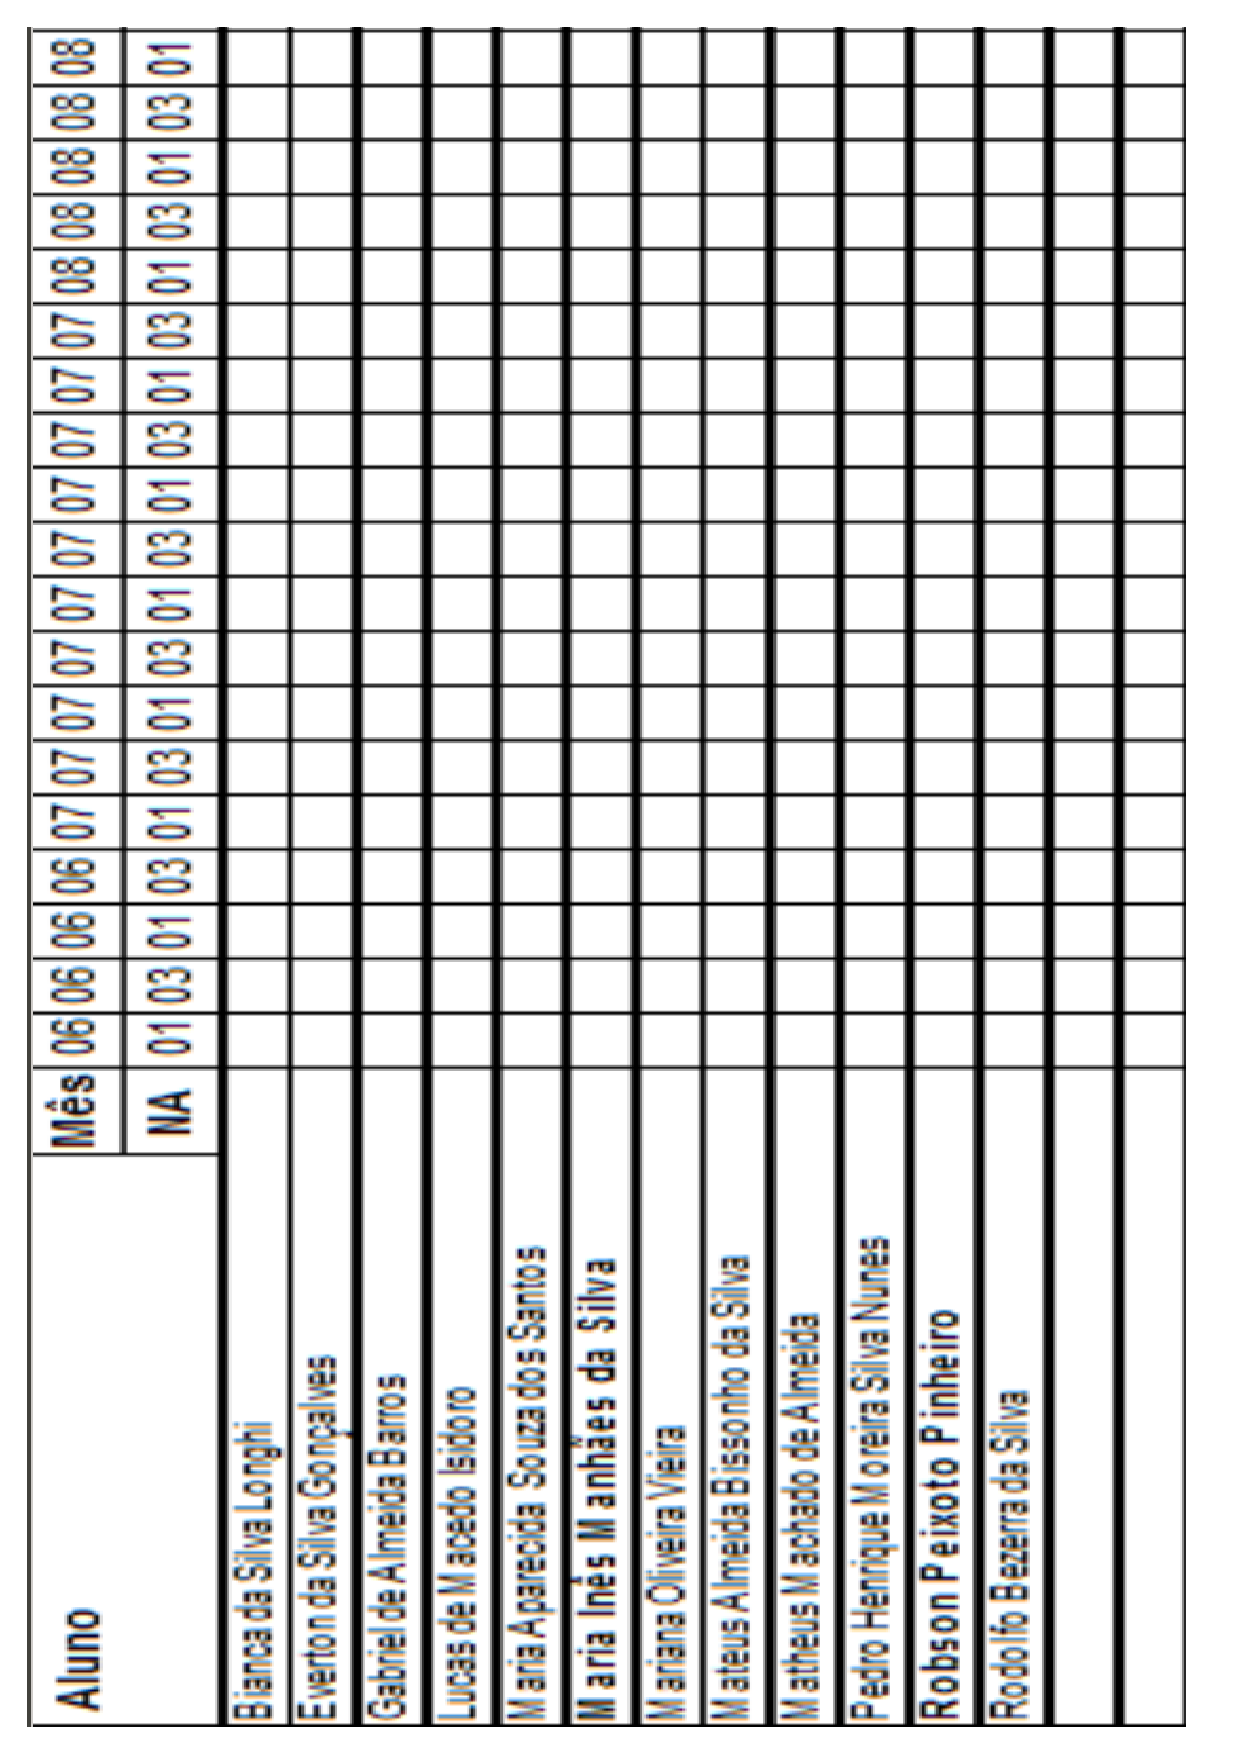
\includepdf{pre/FolhaAprovacaoAssinada}
% \end{folhadeaprovacao}

\begin{folhadeaprovacao}

\setlength{\ABNTEXsignwidth}{14cm}

    \begin{center}
    {\ABNTEXchapterfont\large\imprimirautor}

    \vspace*{\fill}\vspace*{\fill}
    {\ABNTEXchapterfont\bfseries\Large\imprimirtitulo}
    \vspace*{\fill}
    
    \hspace{.45\textwidth}
    \begin{minipage}{.5\textwidth}
        \imprimirpreambulo
    \end{minipage}%
    \vspace*{\fill}
   
   \end{center}
 
 
   \begin{center}
    \imprimirlocal, \imprimirdia ~de \imprimirmes ~de \imprimirano.
   \end{center}
   
   % Instituto Federal Fluminense (IFF)
   \assinatura{\textbf{\imprimirorientador \, (orientador)} \\ Instituto Federal Fluminense (IFF)}
   \assinatura{\textbf{Prof. D.Sc. Fernando Luiz de Carvalho e Silva} \\ Instituto Federal Fluminense (IFF)}
   \assinatura{\textbf{Prof. D.Sc. Ana Silvia Ribeiro Escocard Santiago} \\ Instituto Federal Fluminense (IFF)}

   \begin{center}
    \vspace*{0.5cm}
    {\ABNTEXchapterfont\large\imprimirlocal}
    \par
    {\ABNTEXchapterfont\large\imprimirdata}
    \vspace*{1cm}
  \end{center}
  
\end{folhadeaprovacao}


\begin{agradecimentos}

Em primeiro lugar, agradecemos a Deus, por nos dar força, fé e sabedoria para superar todos os desafios e dificuldades ao longo de nossa jornada acadêmica.

Agradecemos de maneira profunda e especial às nossas famílias, nossos alicerces. Em especial às nossas mães, que sempre nos apoiaram com amor incondicional em cada passo desta jornada. Somos imensamente gratos por todo o sacrifício, carinho e dedicação. Em particular, um de nós presta uma homenagem carinhosa à sua bisavó, cuja memória e legado serviram como uma silenciosa e constante fonte de inspiração. Se hoje celebramos esta conquista, é porque tivemos o privilégio de contar com o suporte de vocês.

Ao nosso orientador, Prof. Me. Ronaldo Amaral Santos, expressamos nossa mais profunda gratidão. Seu apoio, orientação precisa e ensinamentos foram fundamentais não apenas para a condução deste trabalho, mas para nosso crescimento como pesquisadores. Agradecemos por sua paciência, dedicação e pelo conhecimento compartilhado.

Gostaríamos de registrar um agradecimento especial ao Prof. Dr. Rogerio Atem. A oportunidade de participar dos projetos de bolsa sob sua mentoria no polo de inovação nos proporcionou nossas primeiras experiências práticas, sendo um passo fundamental para a aplicação dos conhecimentos teóricos e para o despertar de nossa paixão pela tecnologia. Sua confiança foi essencial em nosso início de carreira.

Agradecemos a todos os professores do Instituto Federal Fluminense que, ao longo do curso, compartilharam seus conhecimentos e nos inspiraram, bem como aos nossos colegas e amigos, que tornaram a jornada mais leve com momentos de companheirismo e apoio mútuo.

Por fim, esta conquista reforça nossa crença de que a educação é a chave não apenas para atingir objetivos pessoais, mas para transformar a sociedade em um lugar mais próspero, solidário e justo.

\end{agradecimentos}

\begin{resumo}

% O comando lipsum abaixo é um gerador automático de texto.
% Substitua-o pelo texto do seu resumo.
% Lembre-se: Um resumo deve ser um parágrafo único que apresente os seguintes tópicos:

% Contexto;
% Problema;
% Objetivo;
% Justificativa;
% Metodologia;
% Resultado;
% Conclusão.

O crescimento exponencial da web, com milhares de sites surgindo diariamente, tem elevado a complexidade do desenvolvimento de aplicações web e evidenciado a importância da escolha adequada da estratégia de renderização de conteúdo. Dentre as principais abordagens estão o \textit{Client-Side Rendering} (CSR) e o \textit{Server-Side Rendering} (SSR), cada uma com características distintas que impactam diretamente a performance, a experiência do usuário (UX), a escalabilidade e a otimização para motores de busca (SEO). Este trabalho tem como objetivo principal realizar uma análise comparativa entre CSR e SSR, destacando seus efeitos técnicos e funcionais em aplicações web modernas. A justificativa fundamenta-se na lacuna de estudos de caso práticos e aprofundados, especialmente no contexto nacional, que analisem criticamente os impactos reais da adoção dessas abordagens. A metodologia adotada envolveu fundamentação teórica, mapeamento sistemático da literatura com uso da técnica \textit{PICOC}, e a implementação de um estudo de caso realista, com coleta de métricas de desempenho, tempo de carregamento, impacto em SEO e UX. Os resultados apontaram que, embora o CSR seja mais vantajoso em aplicações altamente interativas, o SSR apresenta melhor desempenho inicial e maior indexabilidade. Conclui-se que a escolha entre CSR e SSR deve considerar o perfil do sistema, a infraestrutura disponível e os objetivos estratégicos do projeto, sendo muitas vezes recomendável a adoção de soluções híbridas.

\textbf{Palavras-chave: } Renderização do lado do cliente, CSR,renderização do lado do servidor, SSR,  Renderização Web, Desempenho, SEO, UX.

\end{resumo}




\begin{resumo}[Abstract]
\begin{otherlanguage*}{english}
    
With the growing complexity of web applications and the demand for rich, high-performance user experiences, the choice of a content rendering strategy has become a fundamental architectural decision. In this context, \textit{Client-Side Rendering} (CSR) and \textit{Server-Side Rendering} (SSR) emerge as the main approaches, each with significant \textit{trade-offs}: CSR favors continuous interactivity, while SSR optimizes initial load times and search engine optimization (SEO). The literature, however, lacks practical case studies that directly and controllably compare their impacts.

Aiming to fill this gap, this work presents a detailed comparative analysis based on a realistic case study: the development of a news platform in two functionally identical versions, one with React (CSR) and the other with Next.js (SSR). Through the collection of \textit{Core Web Vitals} metrics in a controlled environment using Docker containers, the research empirically evaluates the effects of each architecture on performance and user experience. The study thus seeks to offer a clear contribution to understanding the application scenarios for each approach, helping development teams make more informed and strategic decisions.

\textbf{Keywords:} Client-side rendering, CSR, Server-side rendering, SSR, Web Rendering, Performance, SEO, UX.
\end{otherlanguage*}
\end{resumo}


% não é necessário alterar este arquivo

\listoffigures*
\clearpage


% não é necessário alterar este arquivo


\hidefromtoc
\listofquadros
\writetotoc
\clearpage

% % não é necessário alterar este arquivo

\listoftables*
\clearpage


% não é necessário alterar este arquivo

\listofcodigos*




% \printglossaries
\printglossary

\setglossarypreamble[acronym]{%
	\glsresetentrycounter
}
\setglossarystyle{long3col}
\printnoidxglossary[type=acronym]

\clearpage



\setglossarypreamble[symbols]{%
	\glsresetentrycounter
}

\setglossarystyle{long3col}

\printnoidxglossary[type=symbols]

\clearpage



 %%%%%%%%%%%%  This Produces Table Of Contents %%%%%%%%%%%%%%

\vspace{\baselineskip}
\setlength{\parskip}{0.0pt}

\begin{Center}
\end{Center}\par


\vspace{\baselineskip}
\setlength{\parskip}{9.96pt}


\tableofcontents*

\clearpage

 %%%%%%%%%%%%  Starting New Page here %%%%%%%%%%%%%%


\textual

\chapter{Introdução}
\label{cap:introducao}

\section{Problema e contexto}
O crescimento acelerado da web e o aumento da complexidade das aplicações modernas impuseram novos desafios ao desenvolvimento e à entrega de conteúdos na internet. Com o crescimento exponencial da web, estima-se que aproximadamente 252 mil novos sites sejam desenvolvidos diariamente, demonstrando não apenas a rapidez com que aplicações são criadas, mas também a necessidade crescente de estratégias eficientes para otimização de desempenho e escalabilidade \cite{dataInternetUsage}. A escolha da abordagem de renderização tornou-se um fator determinante para a experiência do usuário e a escalabilidade dos sistemas. Inicialmente, os sites eram compostos por páginas estáticas, cujo conteúdo era carregado diretamente do servidor. Com a evolução das tecnologias frontend, novas abordagens surgiram, destacando-se \english{\acrfull{csr}} e \english{\acrfull{ssr}}. Cada uma dessas técnicas possui características específicas que influenciam diretamente o desempenho e a experiência do usuário.

A performance em websites é um fator determinante para o sucesso de qualquer aplicação web. O desempenho, frequentemente medido pelo tempo de carregamento das páginas, desempenha um papel fundamental na experiência do usuário e na taxa de conversão de visitantes \cite{webPerformance}. Uma página que carrega rapidamente proporciona uma navegação mais fluida, reduzindo a taxa de rejeição e aumentando a retenção de usuários. Além disso, o desempenho da página não se limita a impactar a experiência do usuário, mas também interfere diretamente no \english{\acrfull{seo}}, tornando-se um critério essencial de indexação e ranqueamento em plataformas como o Google \cite{google}.

Um exemplo notável de desafios enfrentados na escolha da estratégia de renderização ocorreu no \emph{Twitter}. Em 2010, a empresa lançou uma nova versão de sua plataforma, conhecida como New Twitter, que utilizava extensivamente a renderização no lado do cliente (\acrshort{csr}) para aprimorar a interatividade e a experiência do usuário. No entanto, essa abordagem resultou em problemas significativos de desempenho, especialmente para usuários com conexões de internet mais lentas ou dispositivos menos potentes. Além disso, a dependência intensa de JavaScript dificultou a indexação de conteúdo pelos mecanismos de busca, impactando negativamente a otimização para motores de busca (\acrshort{seo}) \cite{twitter}. Reconhecendo essas limitações, o Twitter decidiu retornar à renderização no lado do servidor (\acrshort{ssr}) em 2012, visando melhorar o desempenho e a acessibilidade de sua plataforma.

A arquitetura de frontend desempenha papel fundamental ao definir o fluxo de desenvolvimento e a escolha entre \acrshort{csr} e \acrshort{ssr}, sendo indispensável a adoção de um sistema modular e eficiente, capaz de ser mantido e escalado de forma sustentável \cite{frontendGodbolt}. Na abordagem \acrshort{csr}, a renderização ocorre diretamente no navegador do usuário, reduzindo a carga no servidor, mas exigindo mais processamento no cliente; já na \acrshort{ssr}, o conteúdo é gerado no servidor antes de ser enviado ao cliente, o que proporciona carregamento mais rápido e melhor desempenho em dispositivos menos potentes. A decisão entre essas estratégias está diretamente ligada à performance da aplicação e deve considerar fatores como tempo de carregamento, complexidade da página e número de requisições HTTP \cite{webPerformance}, já que diferentes abordagens afetam não apenas a experiência do usuário, mas também os custos operacionais e a infraestrutura necessária para suportar a aplicação.

\section{Justificativa}


\section{Objetivos}

\subsection{Objetivo Geral}


\subsection{Objetivos Específicos}
\begin{itemize}
\item item 1
\item item 2
\item item 3
\end{itemize}

\section{Metodologia}


\section{Estrutura do Trabalho}



\chapter{Fundamentação Teórica}
\label{cap:fundamentacao}

Este capítulo apresenta os conceitos de \english{\acrfull{csr}} e \english{\acrfull{ssr}}, abordando os princípios fundamentais do desenvolvimento web relacionados à renderização de conteúdo. Também são discutidos aspectos como \acrshort{seo}, desempenho, infraestrutura de serviços e impacto na experiência do usuário, estabelecendo a base teórica para o estudo de caso desenvolvido neste trabalho.

\section{Fundamentos de Desenvolvimento Web}
\label{sec:fundamentos-devweb}
Para entender como as abordagens \acrshort{ssr} e \acrshort{csr} se inserem no cenário de desenvolvimento web, é fundamental revisar protocolos, modelos de arquitetura e ferramentas.
Os fundamentos de desenvolvimento web englobam os princípios, tecnologias e práticas essenciais para a criação e manutenção de aplicações acessíveis via internet. 

O desenvolvimento web baseia-se na arquitetura cliente-servidor, onde o cliente (geralmente um navegador) solicita recursos ao servidor, que processa essas requisições e retorna os dados necessários. Essa interação é mediada por protocolos como o 
\english{\acrfull{http}} , que define as regras de comunicação entre cliente e servidor.

As tecnologias fundamentais incluem \english{\acrfull{html}} para estruturação do conteúdo, \english{\acrfull{css}} para estilização e JavaScript para interatividade. Essas linguagens permitem a construção de interfaces dinâmicas e responsivas. Além disso, o desenvolvimento web envolve práticas como controle de versão, testes automatizados e integração contínua, que garantem a qualidade e a escalabilidade das aplicações \cite{fundamentosDevWeb}. 

\subsection{Arquitetura Cliente-Servidor}
\label{subsec:Arquitetura Cliente-Servidor}

A arquitetura cliente-servidor é um modelo amplamente adotado no desenvolvimento de aplicações web, caracterizado pela separação entre dois componentes principais: o \textbf{cliente}, responsável pela interface com o usuário, e o \textbf{servidor}, que processa solicitações e fornece os recursos necessários \cite{clienteServidorControlNet}.

Nesse modelo, os clientes como navegadores em diferentes dispositivos enviam requisições através da internet, enquanto os servidores respondem disponibilizando dados, arquivos e serviços. Essa divisão de responsabilidades favorece a escalabilidade, facilita a manutenção e permite que cliente e servidor operem em plataformas distintas~\cite{fundamentosDevWeb}.

A Figura~\ref{fig:cliente-servidor} ilustra, de forma simplificada, esse fluxo de comunicação entre cliente e servidor.

\begin{figure}[H]
  \centering
  \caption{Comunicação entre cliente e servidor.}
  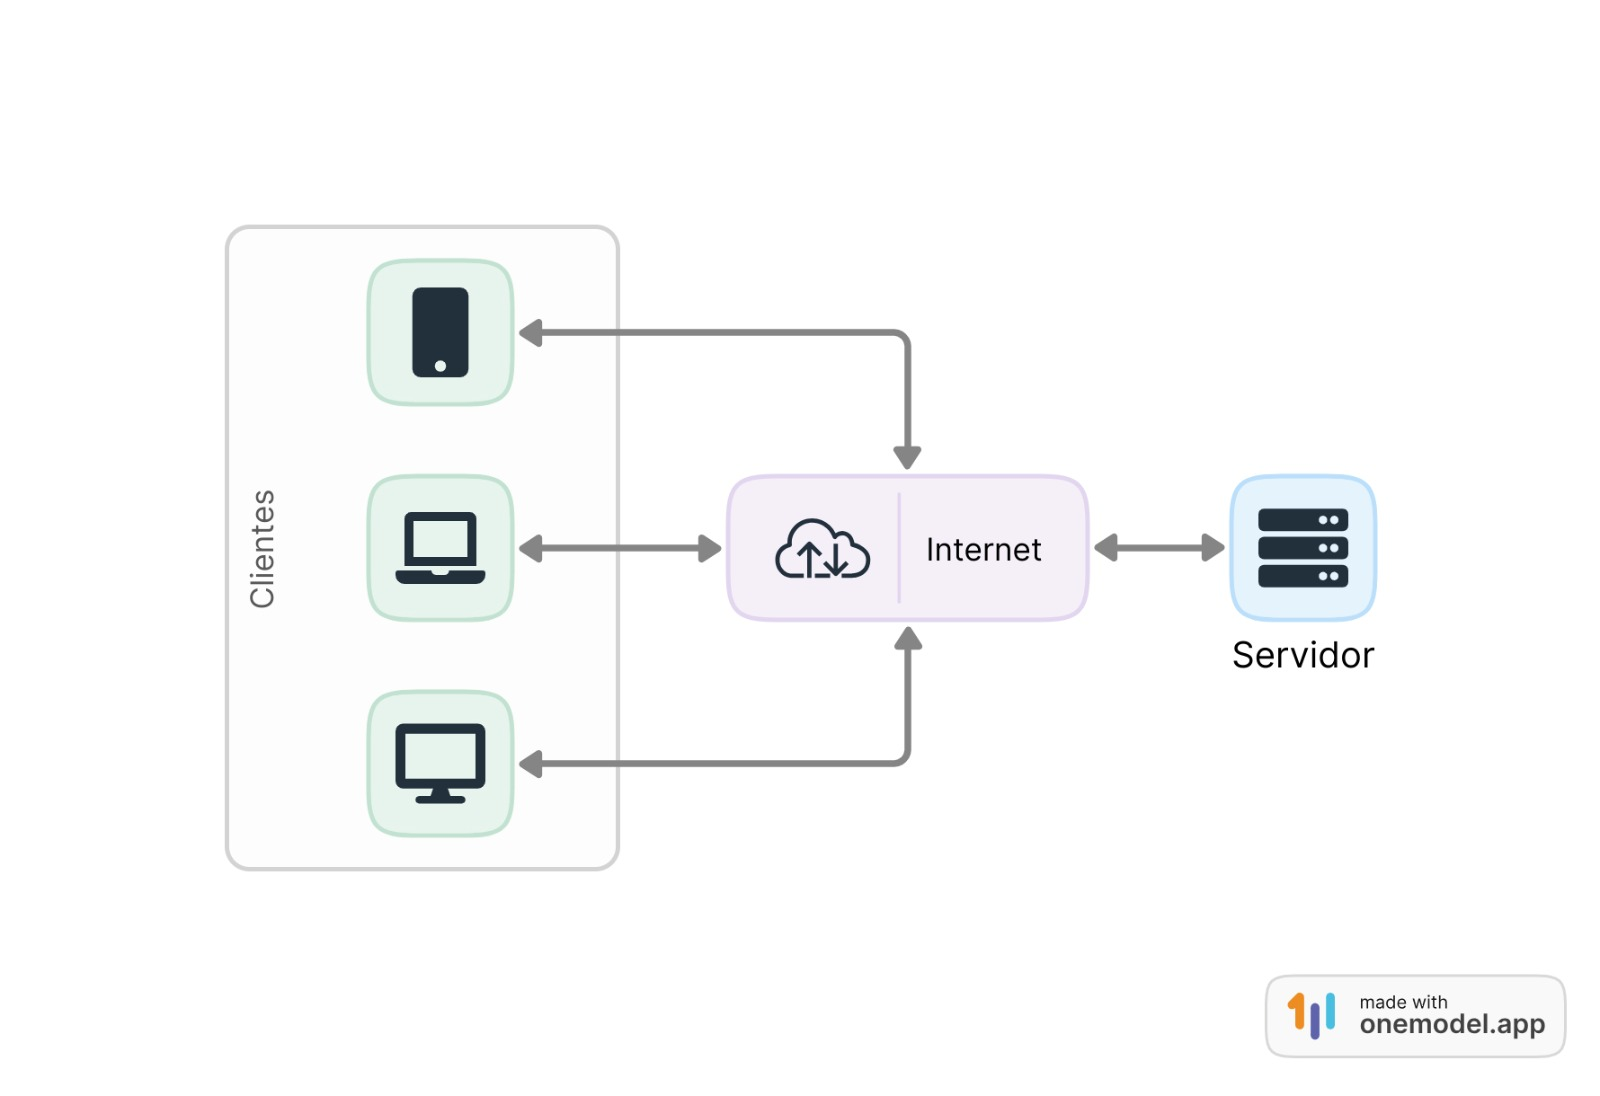
\includegraphics[width=0.8\textwidth]{media/cliente_servidor.jpeg}
  \legend{Fonte: \cite{fundamentosDevWeb} }
  \label{fig:cliente-servidor}
\end{figure}


A arquitetura cliente-servidor apresenta características que contribuem para sua ampla adoção em aplicações web. Entre elas, destaca-se a \textbf{distribuição de responsabilidades}, onde o servidor gerencia dados e processos mais complexos, enquanto o cliente lida com a interface e a interação com o usuário. 

Outro ponto relevante é a \textbf{independência entre plataformas}, possibilitada pelo uso de protocolos padronizados, o que permite a comunicação entre diferentes dispositivos e sistemas operacionais. Além disso, esse modelo favorece a \textbf{facilidade de manutenção}, já que atualizações podem ser feitas no servidor sem necessidade de intervenção nos dispositivos dos usuários.

Na web, essa arquitetura é implementada por padrão: navegadores atuam como clientes, enviando requisições \acrshort{http} que são processadas por servidores, os quais respondem com páginas e recursos solicitados~\cite{fundamentosDevWeb}.


\subsection{Protocolo \acrshort{http}}
\label{subsec:http}
O \textbf{Protocolo de Transferência de Hipertexto} (\acrshort{http}) é a base da comunicação na World Wide Web, definindo como clientes (navegadores) e servidores trocam informações. Ele especifica a estrutura das requisições e respostas, permitindo a recuperação de recursos como documentos \acrshort(html), imagens e vídeos \cite{mdn_http}.


 O \textbf{Funcionamento do \acrshort{http}}opera no modelo cliente-servidor, onde o cliente inicia uma requisição e o servidor responde com os recursos solicitados ou mensagens de erro, se aplicável. Cada interação consiste em uma mensagem de requisição do cliente e uma mensagem de resposta do servidor. As mensagens \acrshort{http} são compostas por:

\begin{itemize}
    \item \textbf{Linha de início:} Indica o método \acrshort{http} (como \texttt{GET} ou \texttt{POST}) e o caminho do recurso.
    \item \textbf{Cabeçalhos:} Fornecem informações adicionais sobre a requisição ou resposta, como tipo de conteúdo e codificação.
    \item \textbf{Corpo:} Contém os dados enviados ou recebidos, sendo opcional dependendo do método utilizado.
\end{itemize}

\begin{flushright}
    \cite{mdn_http}
\end{flushright}


\textbf{Métodos \acrshort{http}} são operações definidas pelo protocolo que especificam a ação a ser realizada em um recurso. Os métodos mais comuns incluem:

\begin{itemize}
    \item \textbf{GET:} Solicita a representação de um recurso específico. Requisições GET devem ser utilizadas apenas para recuperar dados.
    \item \textbf{POST:} Envia dados ao servidor para processamento, como o envio de formulários.
    \item \textbf{PUT:} Atualiza um recurso existente ou cria um novo se não existir.
    \item \textbf{DELETE:} Remove um recurso específico.
    \item \textbf{HEAD:} Similar ao GET, mas solicita apenas os cabeçalhos da resposta, sem o corpo.
\end{itemize}
Cada método possui uma finalidade específica e deve ser utilizado conforme a necessidade da aplicação \cite{wikipedia_http}.


\textbf{Códigos de Status \acrshort{http}} são códigos de três dígitos que indicam o resultado de uma requisição feita pelo cliente ao servidor. Eles são agrupados em cinco classes principais:

\begin{itemize}
    \item \textbf{1xx (Informativo):} Indica que a requisição foi recebida e o processo continua.
    \item \textbf{2xx (Sucesso):} Indica que a requisição foi bem-sucedida. Exemplo: 200 OK.
    \item \textbf{3xx (Redirecionamento):} Indica que é necessário tomar medidas adicionais para completar a requisição. Exemplo: 301 Moved Permanently.
    \item \textbf{4xx (Erro do Cliente):} Indica que houve um erro na requisição do cliente. Exemplo: 404 Not Found.
    \item \textbf{5xx (Erro do Servidor):} Indica que o servidor falhou ao processar uma requisição válida. Exemplo: 500 Internal Server Error.
\end{itemize}

Esses códigos auxiliam na identificação e resolução de problemas durante a comunicação \acrshort{http} \cite{mdn_http}.


\textbf{Evolução do \acrshort{http}} refere-se às revisões progressivas do protocolo com o objetivo de aprimorar sua eficiência e desempenho ao longo do tempo. As principais versões são:

\begin{itemize}
    \item \textbf{HTTP/1.0:} Primeira versão oficial do protocolo, em que cada requisição exigia uma nova conexão com o servidor.
    \item \textbf{HTTP/1.1:} Introduziu conexões persistentes, permitindo múltiplas requisições por conexão. Trouxe também melhorias no controle de cache e suporte a novos métodos.
    \item \textbf{HTTP/2:} Implementou multiplexação, compressão de cabeçalhos e priorização de fluxos, resultando em uma transferência de dados mais rápida e eficiente.
    \item \textbf{HTTP/3:} Baseado no protocolo \acrshort{quic}, substitui o \acrshort{tcp} pelo \acrshort{udp}, oferecendo conexões mais rápidas e seguras, com menor latência e melhor desempenho em redes instáveis.
\end{itemize}

Essas atualizações refletem a evolução das necessidades da web e a busca por protocolos mais robustos e otimizados \cite{cloudflare_http}.

\textbf{\acrshort{http} e \acrshort{https}} representam protocolos utilizados para comunicação na web, com a principal distinção centrada na segurança da transmissão dos dados.

O \textbf{\english{\acrfull{https}}} é uma extensão do \acrshort{http} que adiciona uma camada de proteção por meio do protocolo \english{\acrfull{tls}} ou, anteriormente, \english{\acrfull{ssl}}. Essa camada de segurança garante a confidencialidade, integridade e autenticidade dos dados trafegados entre cliente e servidor. 

A criptografia utilizada impede que terceiros acessem ou modifiquem as informações transmitidas, o que é fundamental em transações sensíveis, como cadastros, pagamentos e autenticações. Além disso, o uso de \textit{certificados digitais} garante que o site visitado é realmente aquele que afirma ser, protegendo os usuários contra ataques como o \textit{man-in-the-middle}\footnote{Um ataque \textit{man-in-the-middle} ocorre quando um invasor intercepta e possivelmente altera a comunicação entre duas partes que acreditam estar se comunicando diretamente. Isso pode permitir que o invasor capture informações sensíveis ou injete dados maliciosos na comunicação.\cite{wikipedia_man_in_the_middle}}.

Enquanto o \acrshort{http} tradicional opera normalmente na porta \acrshort{tcp} 80, o \acrshort{https} utiliza, por convenção, a porta 443. Atualmente, o uso do \acrshort{https} é fortemente recomendado e até exigido por navegadores modernos como padrão de segurança para qualquer aplicação web, contribuindo para a privacidade e confiança dos usuários \cite{wikipedia_http}.

\subsection{\acrshort{html}, \acrshort{css} e JavaScript}
\label{subsec:html-css-js}


O desenvolvimento frontend, conforme definido por \citeonline{aws_frontend_backend}, refere-se à camada de apresentação de uma aplicação web a interface gráfica com a qual os usuários interagem diretamente, composta por menus, botões, formulários e outros elementos visuais. Essa camada baseia-se em um conjunto de tecnologias fundamentais que operam em conjunto para fornecer estrutura, estilo e interatividade às páginas: \acrshort{html}, \acrshort{css} e JavaScript. Cada uma dessas linguagens desempenha um papel específico e complementar, sendo essenciais tanto em abordagens tradicionais quanto em técnicas modernas como o \acrshort{csr}.


\textbf{\acrfull{html}} é a linguagem de marcação padrão para a criação da estrutura de páginas web. Através de um conjunto de elementos (ou \textit{tags}), o \acrshort{html} organiza e define o conteúdo exibido ao usuário, como textos, imagens, links, formulários e tabelas. Além de estruturar visualmente o documento, o \acrshort{html} também confere semântica aos elementos, facilitando a indexação por motores de busca e promovendo acessibilidade para leitores de tela. Elementos como \texttt{<header>}, \texttt{<main>}, \texttt{<article>} e \texttt{<footer>} exemplificam essa função semântica~\cite{alura_htmlcssjs}.

\textbf{\acrfull{css}} é a linguagem responsável pela estilização das páginas web. Com o \acrshort{css}, define-se a aparência dos elementos estruturados no \acrshort{html}, controlando propriedades visuais como cores, fontes, espaçamentos, tamanhos e posicionamentos. O \acrshort{css} permite ainda a construção de layouts complexos e responsivos, adaptando o conteúdo para diferentes tamanhos de tela e dispositivos. A separação entre estrutura (\acrshort{html}) e estilo (\acrshort{css}) é um dos pilares das boas práticas em desenvolvimento web, promovendo manutenibilidade, reutilização e modularidade do código.

Entre os recursos modernos do \acrshort{css}, destacam-se os seletores avançados, variáveis \acrshort{css}, pseudo-classes, animações e as funcionalidades de \textit{Flexbox} e \textit{Grid}, que facilitam a criação de interfaces ricas e adaptáveis~\cite{herocode_diferencas}.

\textbf{JavaScript} é uma linguagem de programação interpretada, orientada a objetos e baseada em eventos, amplamente utilizada para adicionar interatividade e dinamismo às páginas web. Por meio da manipulação da \textit{\acrfull{dom}}, permite implementar funcionalidades como respostas a cliques, envio de formulários, movimentações do mouse, digitação, animações, validações e atualizações em tempo real, enriquecendo significativamente a experiência do usuário~\cite{alura_htmlcssjs}. Além disso, possibilita o carregamento assíncrono de dados com a técnica \textit{AJAX} (\textit{Asynchronous JavaScript and XML}), evitando recarregamentos completos da página.

JavaScript é uma das três principais tecnologias da World Wide Web, juntamente com \acrshort{html} e \acrshort{css}, sendo essencial tanto em abordagens tradicionais quanto modernas. Nas aplicações baseadas em \acrshort{csr}, essa linguagem tem papel central, pois a renderização das páginas ocorre diretamente no navegador do usuário. Com a evolução do ecossistema JavaScript, surgiram bibliotecas e frameworks robustos como a biblioteca React e os frameworks Vue.js e Angular que facilitam o desenvolvimento de aplicações complexas com componentes reutilizáveis e gerenciamento eficiente de estado.

Adicionalmente, o JavaScript também pode ser executado no lado do servidor (\acrshort{ssr}) por meio de ambientes como o Node.js uma plataforma de código aberto e multiplataforma baseada em eventos e não bloqueante, ideal para aplicações escaláveis e em tempo real~\cite{nodejs2025, js2025}. Isso permite o desenvolvimento de aplicações completas utilizando uma única linguagem em ambas as camadas, cliente e servidor.

A interação entre essas três tecnologias pode ser compreendida por meio de uma analogia: o \acrshort{html} representa a estrutura de um corpo (esqueleto), o \acrshort{css} corresponde à sua aparência externa (pele, roupas, estilo), enquanto o JavaScript age como os músculos e o sistema nervoso, controlando os movimentos e respostas interativas da aplicação. A Figura~\ref{fig:html-css-js} ilustra essa relação.

\begin{figure}[H]
  \centering
  \caption{Analogia entre HTML, CSS e JavaScript e os componentes de um corpo humano.}
  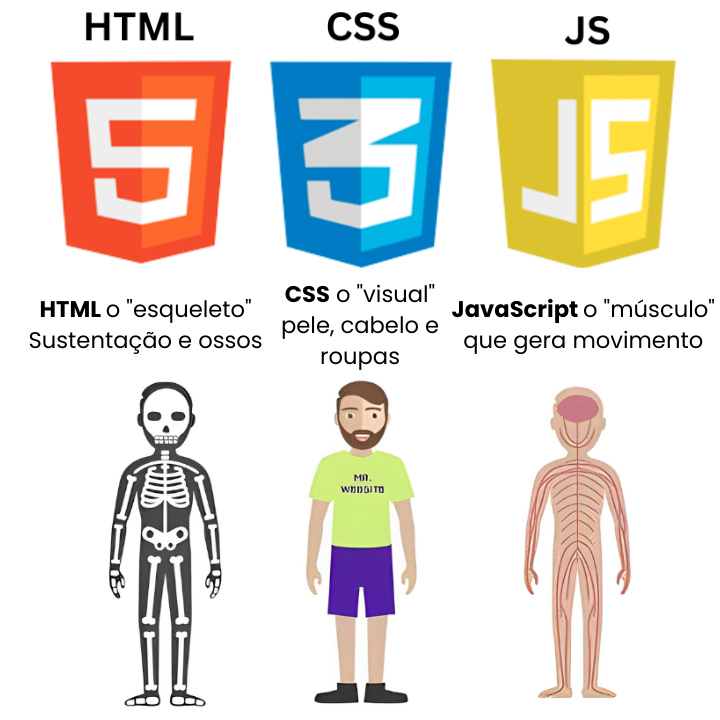
\includegraphics[width=0.6\textwidth]{media/html_css_js_analogia.png}
  \legend{Fonte: \cite{herocode_diferencas}.}
  \label{fig:html-css-js}
\end{figure}

Portanto, o domínio dessas três tecnologias é indispensável para qualquer desenvolvedor web. Elas formam o alicerce sobre o qual se constroem interfaces acessíveis, performáticas e envolventes, sendo empregadas tanto em aplicações renderizadas no servidor (\acrshort{ssr}) quanto no cliente (\acrshort{csr}), com adaptações específicas conforme a abordagem escolhida.



\section{Renderização na Web}
\label{sec:renderizacao-web}

A renderização na Web diz respeito ao processo de transformar dados em conteúdo visual interpretável pelo navegador. A escolha sobre onde e como essa renderização será realizada (seja no cliente, no servidor ou em tempo de build), isso impacta diretamente métricas como tempo de carregamento, interatividade e indexação por mecanismos de busca \cite{osmani2025}.


\subsection{\acrfull{spa} e \acrfull{mpa}}
\label{subsec:spa-mpa}

As arquiteturas \acrfull{spa} e \acrfull{mpa} representam duas abordagens distintas para a estrutura de navegação e carregamento de conteúdo em aplicações web.

As \acrshort{spa}s são aplicações em que a navegação entre páginas ocorre sem recarregamentos completos do navegador. Após o carregamento inicial, todo o conteúdo adicional é gerenciado dinamicamente com JavaScript, o que proporciona uma experiência mais fluida e interativa. Essa abordagem é comumente utilizada em conjunto com a renderização no lado do cliente (\acrshort{csr}) e frameworks como React, Angular ou Vue.js \cite{atori2024}.

Já as \acrshort{mpa}s seguem o modelo tradicional de navegação, em que cada clique em um link leva a uma nova requisição \acrshort{http} e recarregamento completo da página. Essa arquitetura é naturalmente mais compatível com a renderização no lado do servidor (\acrshort{ssr}) e favorece aspectos como \acrshort{seo}, acessibilidade e previsibilidade de comportamento \cite{osmani2025}.

A escolha entre \acrshort{spa} e \acrshort{mpa} está diretamente ligada à estratégia de renderização adotada. As \acrshort{spa}s tendem a oferecer experiências mais ricas e responsivas, mas exigem cuidados extras com desempenho e indexação. Por outro lado, as \acrshort{mpa}s são mais robustas em cenários com grande volume de tráfego e requisitos de otimização para mecanismos de busca.



\subsection{Estratégias e Terminologias de Renderização}
\label{subsec:estrategias-terminologias}

Segundo \citeonline{osmani2025}, é importante distinguir os principais modelos de renderização:


\begin{description}
  \item[\textbf{Client-Side Rendering (CSR)}] 
  O conteúdo da aplicação é gerado dinamicamente no navegador, utilizando JavaScript. A página HTML inicial contém apenas uma estrutura básica com os scripts necessários para montar a interface após o carregamento. É comum em aplicações do tipo SPA (Single Page Application).
  
  \item[\textbf{Server-Side Rendering (SSR)}]
  O servidor monta todo o conteúdo da página em HTML antes de enviá-lo ao cliente. Isso permite uma exibição mais rápida do conteúdo, mesmo em conexões lentas, e melhora a indexação por mecanismos de busca.

  \item[\textbf{Static Site Generation (SSG)}]
  As páginas são geradas de forma estática em tempo de build, com base em dados disponíveis no momento da compilação. O conteúdo é entregue diretamente por uma CDN, garantindo alto desempenho.

  \item[\textbf{Incremental Static Regeneration (ISR)}]
  Introduzido pelo Next.js, o ISR permite que páginas geradas estaticamente possam ser atualizadas de forma incremental, após um período de tempo definido. Isso é feito em segundo plano, sem bloquear o carregamento da página atual. Ideal para sites com atualizações frequentes, mas não críticas em tempo real.

  \item[\textbf{Deferred Static Generation (DSG)}]
  Proposto pelo Gatsby, o DSG difere do ISR por não gerar certas páginas no momento do build. Em vez disso, elas são geradas apenas na primeira requisição (on-demand). Após isso, são armazenadas em cache e servidas como estáticas nas requisições seguintes. É útil em projetos com milhares de páginas de baixo acesso, reduzindo significativamente o tempo de build.
\end{description}

Além dessas abordagens, destaca-se o conceito de \textbf{reidratação}, que consiste em ativar a interatividade de páginas SSR ou SSG no cliente. Esse processo utiliza JavaScript para associar os eventos dinâmicos à estrutura HTML previamente renderizada, sendo essencial para tornar a página interativa após a exibição inicial \cite{osmani2025}.


% \subsection*{Métricas de Desempenho em Aplicações Web}

% A avaliação de desempenho em aplicações web modernas vai além do tempo de carregamento total da página. A experiência do usuário \acrshort{ux}, a capacidade de resposta da interface e a estabilidade visual são aspectos fundamentais. Com o intuito de padronizar essas medições, o Google propôs o conjunto \textbf{Core Web Vitals}, que inclui métricas focadas na percepção do usuário real \cite{osmani2025}. Essas métricas são amplamente aplicadas em ferramentas como \textit{Google Lighthouse}, \textit{PageSpeed Insights} e \textit{WebPageTest} \cite{webvitals2025}.

% Entre as principais métricas de desempenho utilizadas na literatura e em auditorias de performance, destacam-se:

% \begin{description}
%     \item[\textbf{TTFB (Time to First Byte)}] Representa o tempo entre a solicitação do navegador e o recebimento do primeiro byte da resposta do servidor. É um indicativo da latência do backend e da eficiência da entrega do conteúdo inicial.

%     \item[\textbf{FCP (First Contentful Paint)}] Indica o tempo necessário para que qualquer parte visível do conteúdo como texto ou imagem seja renderizada na tela. É essencial para avaliar a percepção inicial de carregamento.

%     \item[\textbf{LCP (Largest Contentful Paint)}] Mede o tempo até o maior elemento visível da página ser exibido, geralmente o conteúdo principal. Um valor abaixo de 2,5 segundos é considerado ideal para uma boa experiência visual inicial.

%     \item[\textbf{TTI (Time to Interactive)}] Reflete o momento em que a página está completamente carregada e pronta para responder às interações do usuário. Um TTI alto pode sinalizar bloqueios na thread principal ou scripts pesados.

%     \item[\textbf{TBT (Total Blocking Time)}] Soma o tempo em que a thread principal esteve ocupada com tarefas longas, impedindo que o usuário interagisse com a página. É um complemento importante ao TTI.

%     \item[\textbf{CLS (Cumulative Layout Shift)}] Avalia a estabilidade visual da página durante o carregamento, medindo alterações inesperadas no layout. Valores acima de 0,1 indicam problemas de usabilidade.
% \end{description}

% Outras métricas relevantes, embora não tão amplamente adotadas nos Core Web Vitals, também são úteis em contextos específicos:

% \begin{itemize}
%     \item \textbf{FID (First Input Delay)}: mede o tempo entre a primeira interação do usuário e a resposta do navegador. Substituído pelo INP nas abordagens mais recentes.
    
%     \item \textbf{INP (Interaction to Next Paint)}: métrica que avalia a latência de todas as interações, fornecendo uma visão mais completa da responsividade.

%     \item \textbf{SI (Speed Index)}: calcula a velocidade com que o conteúdo visível é exibido durante o carregamento.

%     \item \textbf{LCPu (LCP under user timing)}: variação do LCP que considera marcações personalizadas de performance.

%     \item \textbf{RTT (Round-Trip Time)}: tempo de ida e volta da requisição na rede, relevante em diagnósticos de conectividade.
% \end{itemize}

% O domínio dessas métricas é essencial para a compreensão do desempenho percebido pelo usuário final e serve como base para decisões técnicas sobre otimização de aplicações web e escolha de estratégias de renderização.


\subsubsection{Desempenho e Compensações}

A renderização do lado do servidor tende a exibir conteúdo mais rapidamente (menor FCP), favorecendo acessibilidade e \textit{SEO}. No entanto, pode aumentar o TTFB, já que a página precisa ser processada antes de ser enviada \cite{osmani2025}. Já a renderização no cliente pode reduzir o tempo de resposta inicial do servidor, mas exige mais do navegador e aumenta o tempo até a página estar interativa (TTI), especialmente em dispositivos móveis.

Modelos híbridos como SSR com \textit{hydration} tentam unir os benefícios de ambas as abordagens, mas podem causar atrasos na interatividade. Técnicas como \textit{hydration progressiva} ou \textit{streaming} reduzem esses impactos ao ativar partes da interface conforme necessário \cite{osmani2025}.

\subsubsection{Avanços Recentes}

Estratégias mais recentes, como a \textbf{renderização trimórfica}, permitem que a renderização ocorra em três camadas: servidor, cliente e \textit{service worker}. Isso possibilita desempenho superior em acessos repetidos e melhor controle sobre o cache e atualização de conteúdo dinâmico \cite{osmani2025}.

\subsubsection{Impacto em SEO e Indexação}

Segundo \citeonline{osmani2025}, abordagens que entregam HTML completo como SSR e SSG são mais eficazes para indexação por mecanismos de busca. Já modelos que dependem fortemente de JavaScript (CSR) exigem testes adicionais e podem comprometer a visibilidade em sistemas como o Googlebot, especialmente quando há falhas na execução dos scripts.

\begin{figure}[H]
  \centering
  \caption{Comparativo entre estratégias de renderização}
  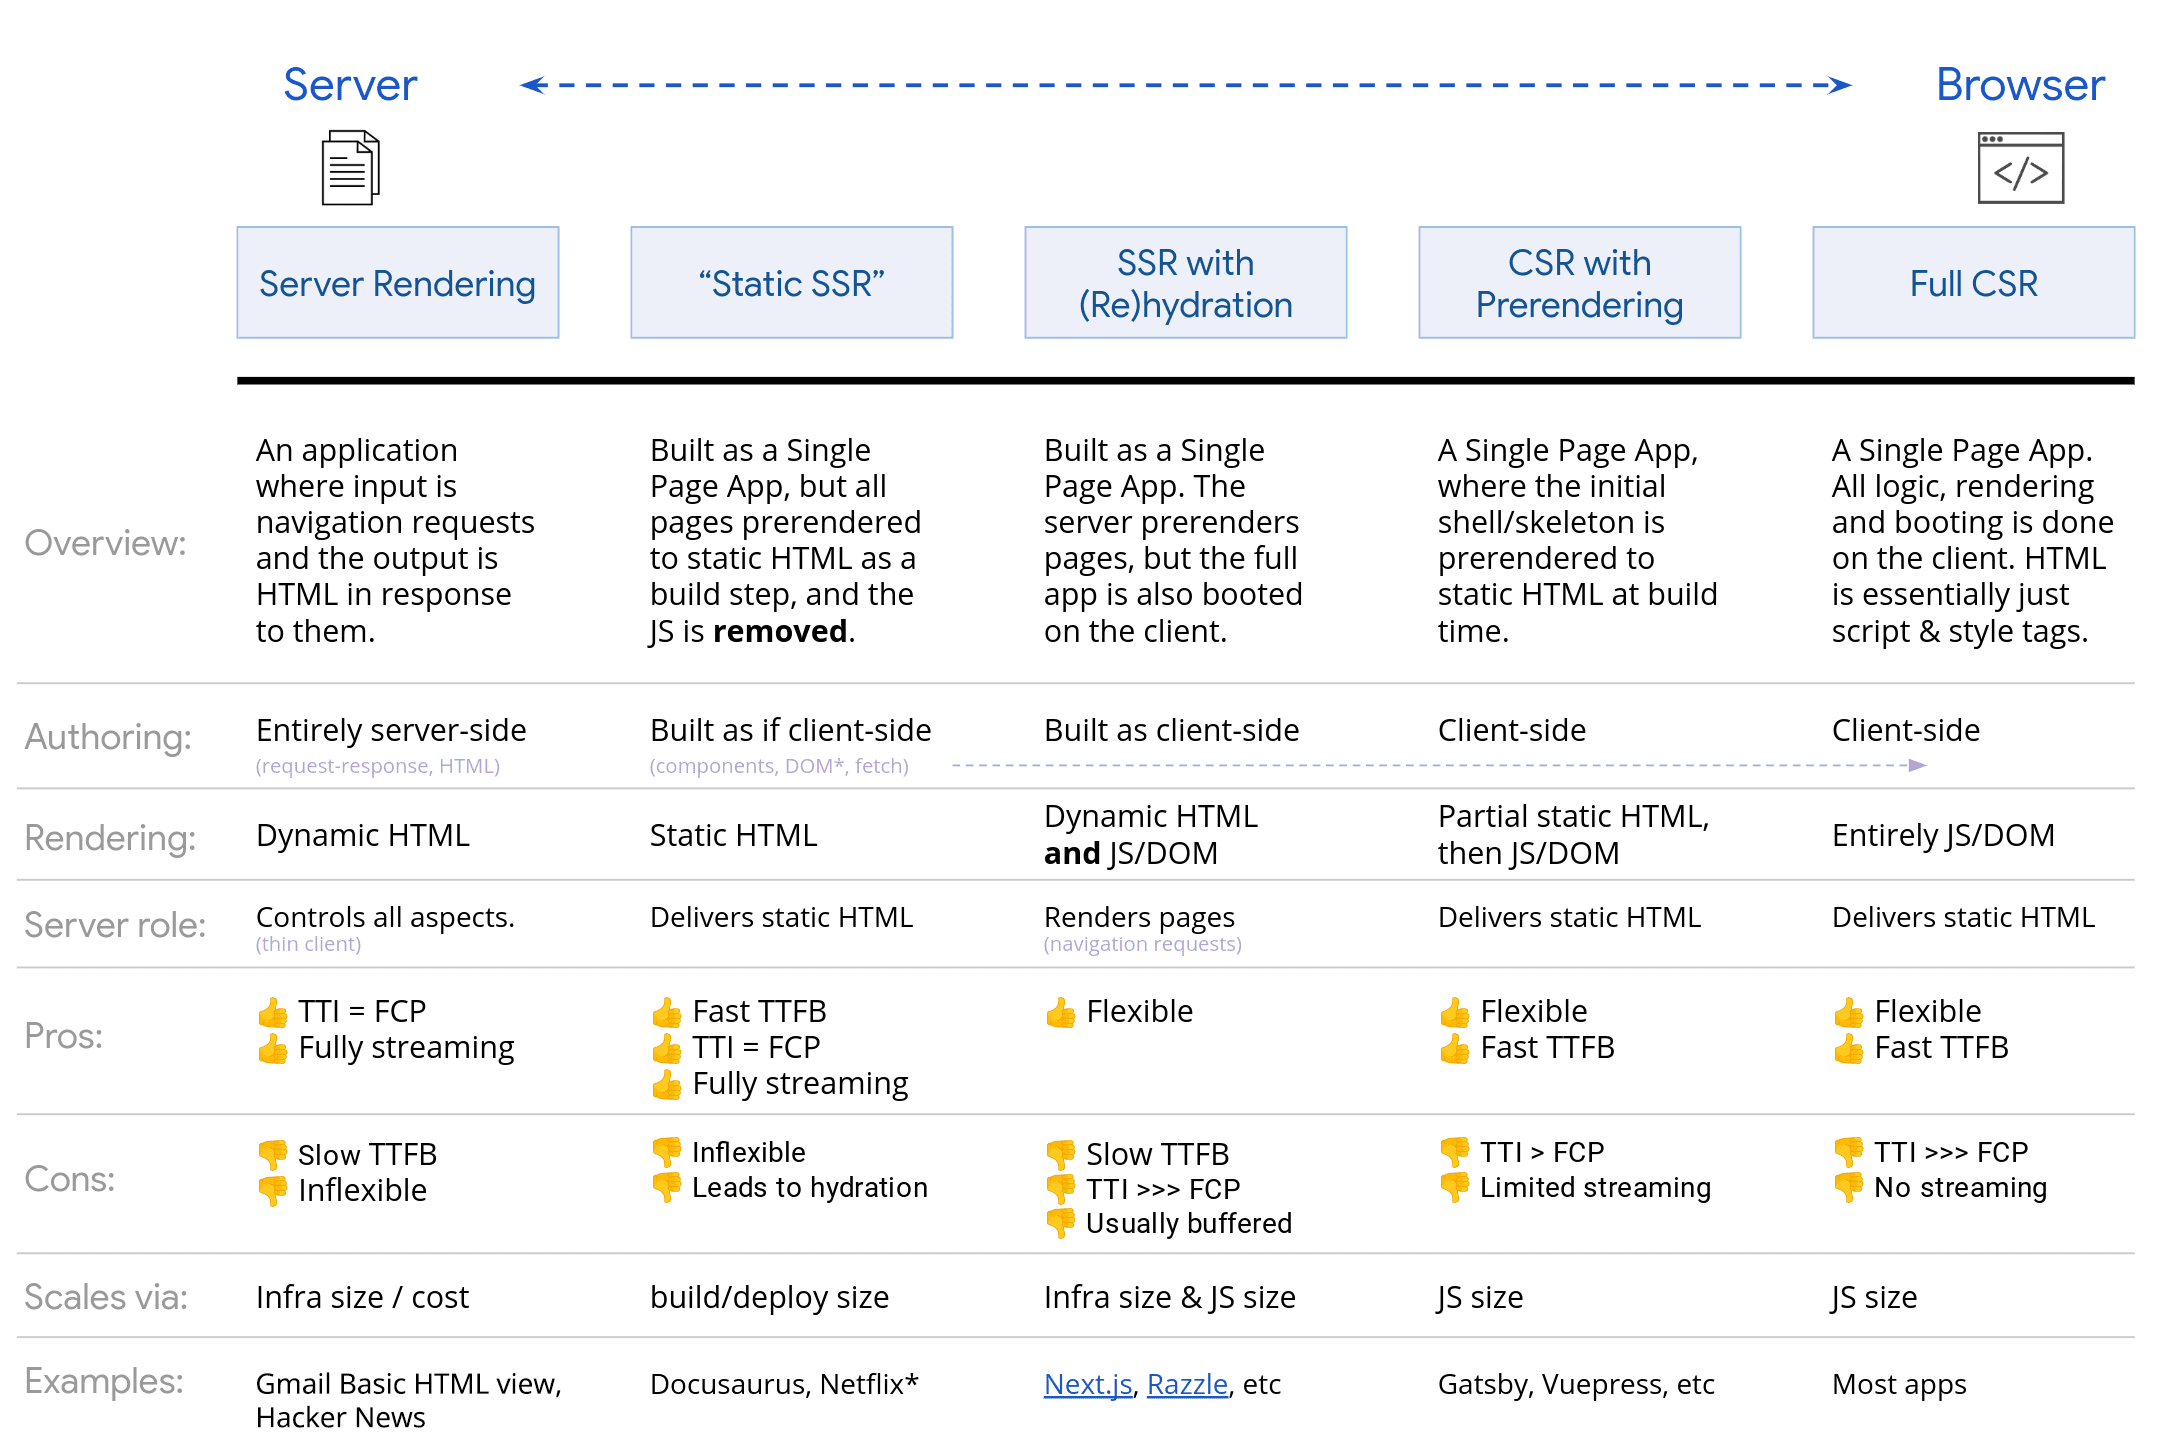
\includegraphics[width=\textwidth]{media/rendering_comparison_table.png}
  \legend{Fonte: Adaptado de \cite{osmani2025}}
  \label{fig:comparativo_renderizacao}
\end{figure}




\subsection{\english{Client-Side Rendering} (\acrshort{csr})}
\label{subsec:csr}

A \textbf{\english{\acrfull{csr}}} é uma técnica em que a geração da interface e do conteúdo final ocorre diretamente no navegador do usuário, utilizando JavaScript. Nessa abordagem, o servidor envia um arquivo \english{\acrfull{html}} mínimo, contendo apenas a estrutura básica da página e referências a arquivos de estilo e scripts.{\cite{atori2024}}

Segundo \citeonline{atori2024}, o processo de renderização no cliente segue as seguintes etapas:

\begin{enumerate}
    \item O servidor envia uma página \acrshort{html} em branco contendo apenas links para os arquivos \english{\acrfull{css}} e JavaScript.
    \item O navegador interpreta o \acrshort{html} e constrói a árvore do \english{\acrfull{dom}}
    \item Os arquivos de estilo (\acrshort{css}) e script (JavaScript) são baixados pelo navegador.
    \item A aplicação é renderizada dinamicamente pelo JavaScript, incluindo elementos visuais como texto, imagens e botões.
    \item O conteúdo da página é atualizado de forma interativa conforme o usuário interage com a aplicação.
\end{enumerate}

Esse modelo é comumente utilizado em aplicações \english{\acrfull{spa}}, nas quais o carregamento inicial é seguido por atualizações dinâmicas sem recarregamento da página. Ferramentas como a biblioteca React, e frameworks como Vue.js, Angular e Svelte são amplamente utilizadas para implementar \acrshort{csr}, permitindo o desenvolvimento de interfaces dinâmicas, interativas e responsivas.


A renderização no lado do cliente (\acrshort{csr}) é especialmente vantajosa em aplicações que exigem alta interatividade e atualizações frequentes de conteúdo, como redes sociais, plataformas de streaming e jogos online. No entanto, essa abordagem pode apresentar desvantagens em termos de desempenho inicial e \acrshort{seo}, uma vez que o conteúdo só é exibido após a execução do JavaScript, o que pode impactar negativamente a indexação por motores de busca e a experiência do usuário em conexões lentas \cite{atori2024}.

\begin{figure}[h!]
    \centering
    \caption{Etapas do método de renderização no lado do cliente}
    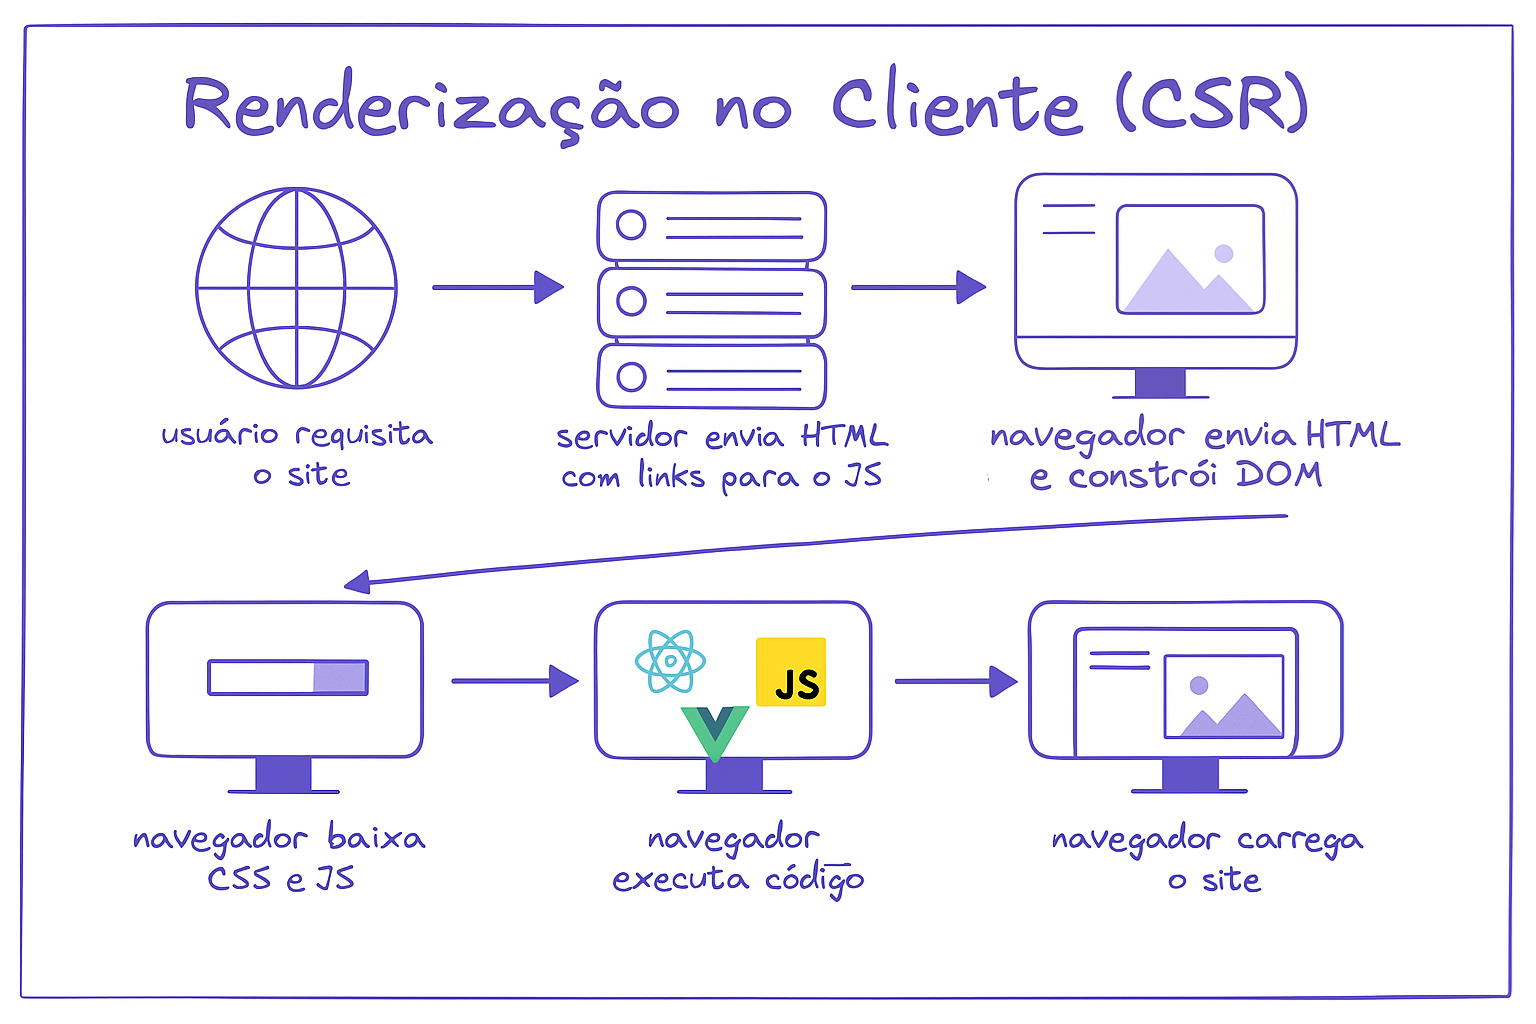
\includegraphics[width=0.8\textwidth]{media/client_side_rendering.png}
    \legend{Fonte: \cite{atori2024} (adaptado)}
    \label{fig:client_side_rendering}
\end{figure}


A \autoref{fig:client_side_rendering} ilustra visualmente o fluxo completo da renderização no lado do cliente (\acrshort{csr}). O processo é iniciado quando o usuário acessa o site em questão. Em resposta, o servidor envia o arquivo \acrshort{html} básico, contendo apenas links para os arquivos de estilo \acrshort{css} e scripts JavaScript responsáveis por carregar e renderizar o conteúdo da aplicação.

Na sequência, o navegador interpreta esse \acrshort{html} e constrói a estrutura da página por meio da árvore \acrshort{dom}. No entanto, o conteúdo principal ainda não está visível. O navegador então precisa baixar os arquivos de estilo (\acrshort{css}) e os scripts JavaScript referenciados no documento inicial.

Com os scripts carregados, o navegador executa o código JavaScript, que normalmente utiliza bibliotecas ou frameworks como React ou Vue para gerar dinamicamente o conteúdo da aplicação. Somente após essa etapa o conteúdo completo do site é finalmente exibido ao usuário, quando o navegador conclui o processo de renderização e o site é carregado completamente.

\begin{codigo}[H]
  \begin{lstlisting}[language=html]
<!DOCTYPE html>
<html lang="en">
<head>
  <meta charset="utf-8">
  <title>CryptoWebsite</title>
  <base href="/">
  <meta name="viewport" content="width=device-width, initial-scale=1">
  <link rel="icon" type="image/x-icon" href="favicon.ico">
  <style>*,*:before,*:after{margin:0;padding:0;box-sizing:border-box;
    font-family:Inter,sans-serif}html{font-size:62.5%}</style>
  <link rel="stylesheet" href="styles.9d4c7581c7242.css">
</head>
<body>
  <app-root></app-root>
  <script src="runtime.6170988ad52a05db.js" type="module"></script>
  <script src="polyfills.574970d5ec4bdb97.js" type="module"></script>
  <script src="main.202d37bb6740400e.js" type="module"></script>
</body>
</html>
\end{lstlisting}
  \caption{Exemplo de HTML mínimo em aplicação Angular com CSR}
  \label{lst:angular_html}
\end{codigo}

Esse padrão é típico de aplicações \acrshort{spa}, onde todo o conteúdo é inserido dinamicamente a partir da execução dos arquivos JavaScript. O elemento \texttt{<app-root>} funciona como ponto de entrada da aplicação, sendo substituído no navegador pelos componentes definidos no framework Angular. {\cite{atori2024}}


\subsection{\english{Server-Side Rendering} (\acrshort{ssr})}
\label{subsec:ssr}

A \textbf{\english{\acrfull{ssr}}} é uma abordagem em que a geração do conteúdo e da interface ocorre integralmente no servidor antes de ser enviada ao navegador do cliente. Ou seja, o servidor processa a lógica da aplicação, obtém dados necessários (por exemplo, em bancos de dados ou \emph{APIs}) e retorna ao cliente um arquivo \english{\acrshort{html}} já renderizado. Dessa forma, o navegador exibe imediatamente a página completa, sem precisar executar \emph{scripts} para montar o conteúdo inicial \cite{atori2024}. 

Segundo \citeonline{atori2024}, o processo típico de renderização no lado do servidor pode ser descrito em quatro etapas principais:

\begin{enumerate}
    \item O servidor recebe uma requisição para uma página e recupera os dados necessários para compor seu conteúdo (por exemplo, produtos de uma base de dados ou artigos de um blog).
    \item O servidor insere esses dados em um \emph{template} \acrshort{html}, gerando a estrutura final da página.
    \item Em seguida, o servidor aplica estilos e finaliza a renderização, resultando em um documento \acrshort{html} completamente montado.
    \item Por fim, esse documento \acrshort{html} é enviado ao navegador do usuário, exibindo a página prontamente, sem a necessidade de executar \emph{JavaScript} durante o carregamento inicial.
\end{enumerate}

Nesse modelo, a fase de hydration\footnote{Hydration é uma etapa essencial no \acrshort{ssr}, em que o JavaScript torna interativo o conteúdo HTML previamente renderizado no servidor.} ocorre após o carregamento inicial da página. costuma ocorrer após a entrega do conteúdo estático. Significa que, assim que o arquivo \acrshort{html} é carregado e mostrado ao usuário, o \emph{JavaScript} do lado do cliente assume o controle para tratar as interações e atualizações dinâmicas subsequentes. Dessa forma, o \acrshort{ssr} beneficia tanto o primeiro acesso (tornando o conteúdo visível rapidamente) quanto o \acrshort{seo}, por exibir ao rastreador dos mecanismos de busca um código \acrshort{html} completo. \cite{atori2024}.

\begin{figure}[H]
  \centering
  \caption{Etapas do método de renderização no lado do servidor}
  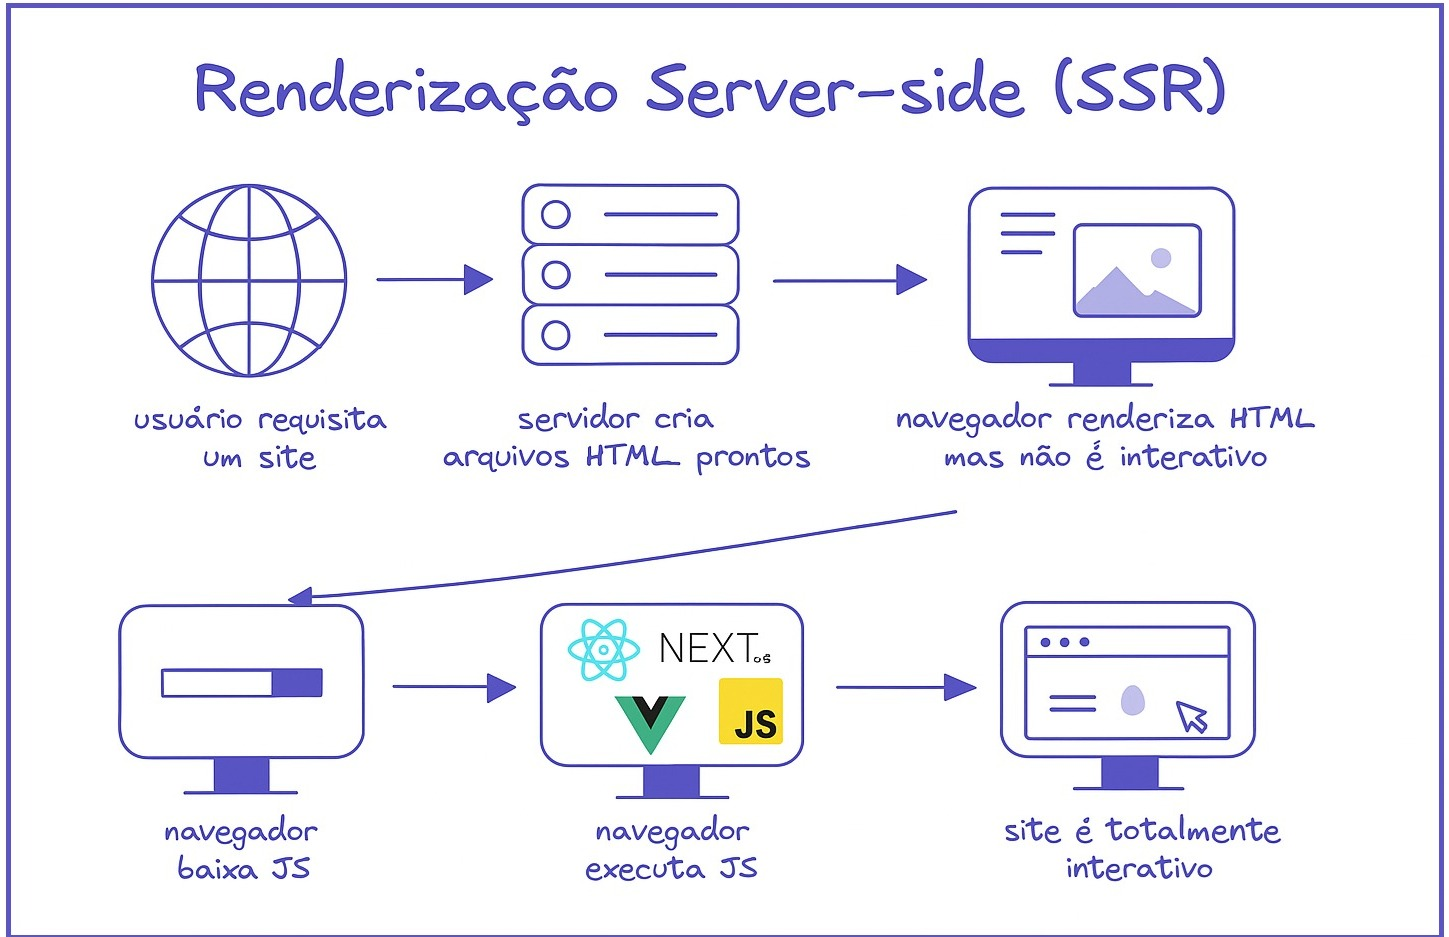
\includegraphics[width=0.8\textwidth]{media/server_side_rendering.jpeg}
  \legend{Fonte: \cite{atori2024} (adaptado)}
  \label{fig:server_side_rendering}
\end{figure}

A \autoref{fig:server_side_rendering} ilustra o fluxo de uma aplicação \acrshort{ssr}. Ao receber a requisição, o servidor gera a página completa em \acrshort{html} e a envia ao cliente. Essa estratégia costuma ser vantajosa em cenários onde o carregamento inicial rápido e a indexação por motores de busca são prioridades, como em sites de e-commerce e páginas de \emph{landing}, permitindo que o usuário visualize o conteúdo de forma imediata. 

\emph{Meta-frameworks} como Next.js, Nuxt.js, SvelteKit, Angular Universal, Remix, Astro e Qwik são amplamente utilizados para construir aplicações com suporte a \acrshort{ssr}. Esses frameworks operam em um nível superior aos tradicionais (como React, Vue ou Svelte), agregando funcionalidades comuns ao desenvolvimento web, como roteamento, pré-renderização, recuperação de dados e \emph{hydration} podendo oferecer uma estrutura mais completa, opinativa e voltada à escalabilidade.

O \acrshort{ssr} é especialmente útil em aplicações que exigem um carregamento inicial rápido e uma boa indexação por motores de busca, como sites de e-commerce, blogs e páginas de \emph{landing}. Essa abordagem permite que o usuário visualize o conteúdo imediatamente, sem esperar pela execução do JavaScript. Além disso, o \acrshort{ssr} melhora a \acrshort{seo}, pois os mecanismos de busca conseguem indexar o conteúdo completo da página desde o início.

No \autoref{cod:nextjs_html}, pode-se observar que o arquivo \acrshort{html} já contém todo o \emph{markup} necessário para exibir o conteúdo da página. Assim que o navegador recebe esse arquivo, o usuário já visualiza o cabeçalho, o texto e o layout definidos. Posteriormente, o \emph{JavaScript} baixado (por exemplo, \texttt{main.js}) pode entrar em ação para lidar com eventos, rotas adicionais e atualizações dinâmicas, caso o desenvolvedor deseje funcionalidades mais interativas.

Por fim, aplicações \acrshort{ssr} tendem a apresentar melhor performance em termos de \emph{time-to-first-byte}\footnote{O \emph{time-to-first-byte} (TTFB) é uma métrica que mede o tempo decorrido entre o envio de uma solicitação HTTP pelo cliente e o recebimento do primeiro byte da resposta do servidor. Um TTFB menor indica maior rapidez na resposta do servidor, impactando diretamente na velocidade de carregamento da página e na experiência do usuário. \cite{ttfb-craig}} e de \emph{indexabilidade}\footnote{A \emph{indexabilidade} refere-se à capacidade dos motores de busca de rastrear e indexar o conteúdo de uma página web. Aplicações SSR, ao fornecerem conteúdo totalmente renderizado no servidor, facilitam a indexação eficiente pelos motores de busca, melhorando a visibilidade nos resultados de pesquisa. \cite{ttfb-oskay}} por motores de busca, ao mesmo tempo em que podem demandar maior carga de processamento no servidor. A escolha por \acrshort{ssr} ou não, portanto, depende do perfil da aplicação e das prioridades do projeto, considerando fatores como volume de tráfego, necessidade de interatividade e requisitos de otimização de conteúdo.

\begin{codigo}[H]
  \begin{lstlisting}[language=html]
    <!DOCTYPE html>
    <html lang="en">
    <head>
      <meta charset="utf-8">
      <title>My SSR App</title>
      <meta name="viewport" content="width=device-width, initial-scale=1">
      <style>
        /* Exemplo simples de estilo inline */
        body {
          margin: 0;
          font-family: Arial, sans-serif;
          background: #f6f6f6;
        }
        h1 { color: #333; }
      </style>
    </head>
    <body>
<!-- Conteudo ja processado e inserido no servidor -->
      <div id="__next">
        <header>
          <h1>Ola, mundo!</h1>
        </header>
        <main>
          <p>Este conteudo foi renderizado no servidor usando Next.js.</p>
        </main>
      </div>
      <!-- Scripts do Next.js para interacao no cliente -->
      <script src="/_next/static/chunks/main.js" defer></script>
    </body>
    </html>
  \end{lstlisting}
  \caption{Exemplo de HTML mínimo em aplicação Next.js com SSR}
  \label{cod:nextjs_html}
\end{codigo}

\subsection{\english{Static Site Generation} (\acrshort{ssg})}
\label{subsec:ssg}

A \textbf{\english{\acrfull{ssg}}} é uma técnica de pré-renderização na qual as páginas da aplicação são geradas estaticamente em tempo de *build* (compilação) e armazenadas como arquivos \acrshort{html}. Ao contrário de abordagens como \acrshort{csr} e \acrshort{ssr}, onde a renderização ocorre no navegador ou sob demanda no servidor, o \acrshort{ssg} permite que o conteúdo já esteja pronto e otimizado para ser entregue diretamente ao navegador, reduzindo a carga do servidor e otimizando o desempenho de carregamento \cite{pahan2021}.

Segundo \citeonline{bose2022}, a renderização no modelo \acrshort{ssg} segue estas etapas principais:

\begin{enumerate}
    \item Durante o processo de construção (build), o gerador de sites estáticos coleta dados de fontes como arquivos locais, \emph{APIs} ou bancos de dados.
    \item Esses dados são utilizados para gerar arquivos \acrshort{html} completos para cada rota da aplicação.
    \item Os arquivos gerados são armazenados e podem ser servidos diretamente por uma \emph{CDN} (Content Delivery Network).
    \item Quando o usuário acessa a aplicação, os arquivos estáticos são entregues instantaneamente, sem necessidade de renderização adicional.
\end{enumerate}

Essa abordagem é ideal para páginas cujo conteúdo não muda com frequência, como blogs, documentações, portfólios e sites institucionais. Como os arquivos são pré-gerados, o tempo de resposta é extremamente rápido, e o \acrshort{seo} é favorecido, já que os mecanismos de busca encontram o conteúdo pronto para indexação.

\begin{figure}[H]
  \centering
  \caption{Etapas do método de geração estática de páginas (SSG)}
  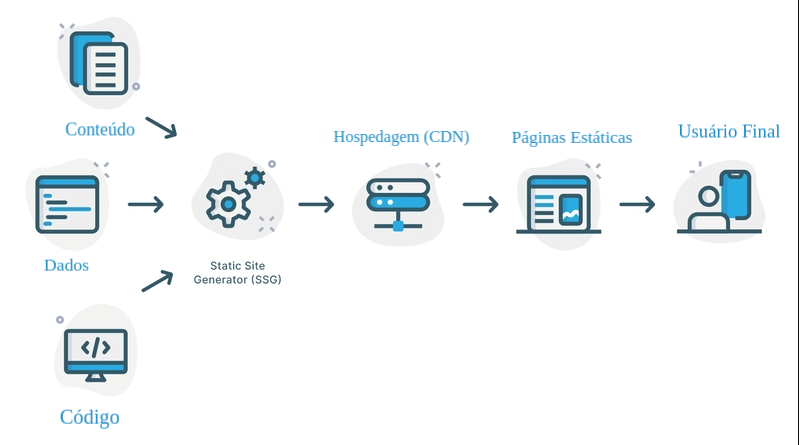
\includegraphics[width=0.8\textwidth]{media/static_site_generation.png}
  \legend{Fonte: \cite{bose2022} (adaptado)}
  \label{fig:ssg}
\end{figure}

Frameworks como Next.js, Gatsby, Hugo e Jekyll oferecem suporte completo ao \acrshort{ssg}, integrando funcionalidades como roteamento dinâmico, \emph{markdown}, e integração com CMSs. No exemplo a seguir, observa-se um documento \acrshort{html} gerado estaticamente por meio de um processo de \emph{build}:

\begin{codigo}[H]
  \begin{lstlisting}[language=html]
<!DOCTYPE html>
<html lang="en">
  <head>
    <meta charset="UTF-8" />
    <meta name="viewport" content="width=device-width, initial-scale=1.0" />
    <title>Post: SSG Example</title>
  </head>
  <body>
    <article>
      <h1>Exemplo de página gerada com SSG</h1>
      <p>Esse conteúdo foi gerado em tempo de build.</p>
    </article>
  </body>
</html>
  \end{lstlisting}
  \caption{Exemplo de HTML estático gerado com SSG}
  \label{cod:ssg_example}
\end{codigo}

A principal limitação do \acrshort{ssg} é a dificuldade em lidar com conteúdos altamente dinâmicos. Alterações nos dados requerem um novo processo de build para que as páginas sejam atualizadas, o que pode ser custoso em grandes aplicações ou com frequência de atualização elevada.

\subsection{\english{Incremental Static Regeneration} (\acrshort{isr})}
\label{subsec:isr}

A \textbf{\english{\acrfull{isr}}} é uma estratégia híbrida introduzida por frameworks como o Next.js, que combina os benefícios da geração estática (\acrshort{ssg}) com a flexibilidade de atualização dinâmica. Com \acrshort{isr}, as páginas são inicialmente geradas estaticamente em tempo de build, mas podem ser revalidadas e regeneradas no servidor de forma incremental e automática, com base em uma estratégia de tempo (ex: a cada 10 segundos) ou conforme novas requisições são feitas \cite{pahan2021}.

De acordo com \citeonline{bose2022}, o fluxo típico do \acrshort{isr} inclui as seguintes etapas:

\begin{enumerate}
    \item No momento do build inicial, as páginas são geradas e armazenadas como arquivos estáticos.
    \item Ao ser requisitada por um usuário, a página é entregue imediatamente, com o conteúdo pré-renderizado.
    \item Se o tempo de revalidação definido (ex: \texttt{revalidate: 60}) tiver expirado, uma nova requisição ao backend é feita em segundo plano.
    \item Essa nova versão da página é armazenada e substitui a anterior, sendo usada em acessos futuros.
\end{enumerate}

Essa abordagem permite obter performance e \acrshort{seo} semelhantes ao \acrshort{ssg}, mas com a vantagem de manter o conteúdo atualizado sem precisar de reconstruções manuais. Por isso, o \acrshort{isr} é ideal para sites que possuem atualizações regulares, porém não críticas em tempo real, como catálogos de produtos, blogs com comentários ou páginas de notícias.

\begin{figure}[H]
  \centering
  \caption{Funcionamento do modelo Incremental Static Regeneration (ISR)}
  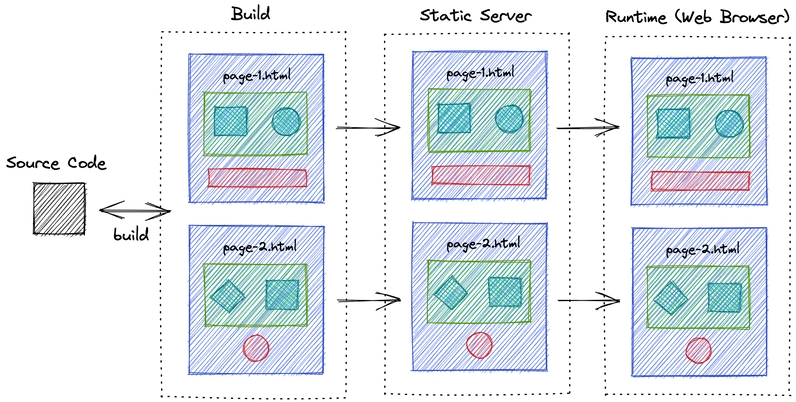
\includegraphics[width=0.8\textwidth]{media/incremental_static_regeneration.png}
  \legend{Fonte: \cite{pahan2021}}
  \label{fig:isr}
\end{figure}

Abaixo, um exemplo típico em Next.js:

\begin{codigo}[H]
  \begin{lstlisting}[language=JavaScript]
      // Funcao usada em getStaticProps
      export async function getStaticProps() {
        const res = await fetch('https://api.exemplo.com/posts')
        const posts = await res.json()

        return {
          props: { posts },
          revalidate: 60, // Pagina sera regenerada a cada 60 segundos
          }
      }
  \end{lstlisting}
  \caption{Exemplo de revalidação de conteúdo com ISR no Next.js}
  \label{cod:isr_next}
\end{codigo}


O \acrshort{isr} representa um meio-termo eficiente entre a performance do \acrshort{ssg} e a flexibilidade do \acrshort{ssr}, oferecendo escalabilidade, \acrshort{seo} eficiente e atualização contínua do conteúdo, sem prejudicar a experiência do usuário.




\subsection{\english{Deferred Static Generation} (\acrshort{dsg})}
\label{subsec:deferred-dsg}

A \textbf{\english{Deferred Static Generation} (DSG)} é uma extensão da estratégia de geração estática proposta pelo framework Gatsby. Essa abordagem permite que certas páginas do site sejam geradas sob demanda ( ou seja, somente no momento em que forem requisitadas pela primeira vez ) em vez de serem construídas durante o processo inicial de build, como ocorre no \acrshort{ssg} tradicional \cite{gatsby2023}.

Segundo a \citeonline{gatsby2023}, o \acrshort{dsg} tem como principal vantagem a capacidade de reduzir significativamente o tempo de build em projetos com um número elevado de páginas, ao evitar a pré-renderização de rotas que têm baixo tráfego ou que não precisam estar imediatamente disponíveis. Após a primeira solicitação, a página é armazenada em cache e, a partir daí, servida como conteúdo estático em acessos subsequentes.

O fluxo típico de geração diferida no \acrshort{dsg} ocorre da seguinte forma:

\begin{enumerate}
    \item Durante o processo de build, apenas páginas prioritárias são pré-geradas.
    \item Páginas marcadas como \texttt{defer} são ignoradas temporariamente.
    \item Quando uma página \acrshort{dsg} é acessada pela primeira vez, um \textit{worker} do Gatsby gera a versão \acrshort{html} da página com base em um componente React (ex: \texttt{about.js}).
    \item A página gerada é armazenada em cache e servida como conteúdo estático nas próximas requisições.
\end{enumerate}

\begin{figure}[H]
  \centering
  \caption{Funcionamento da estratégia Deferred Static Generation (DSG)}
  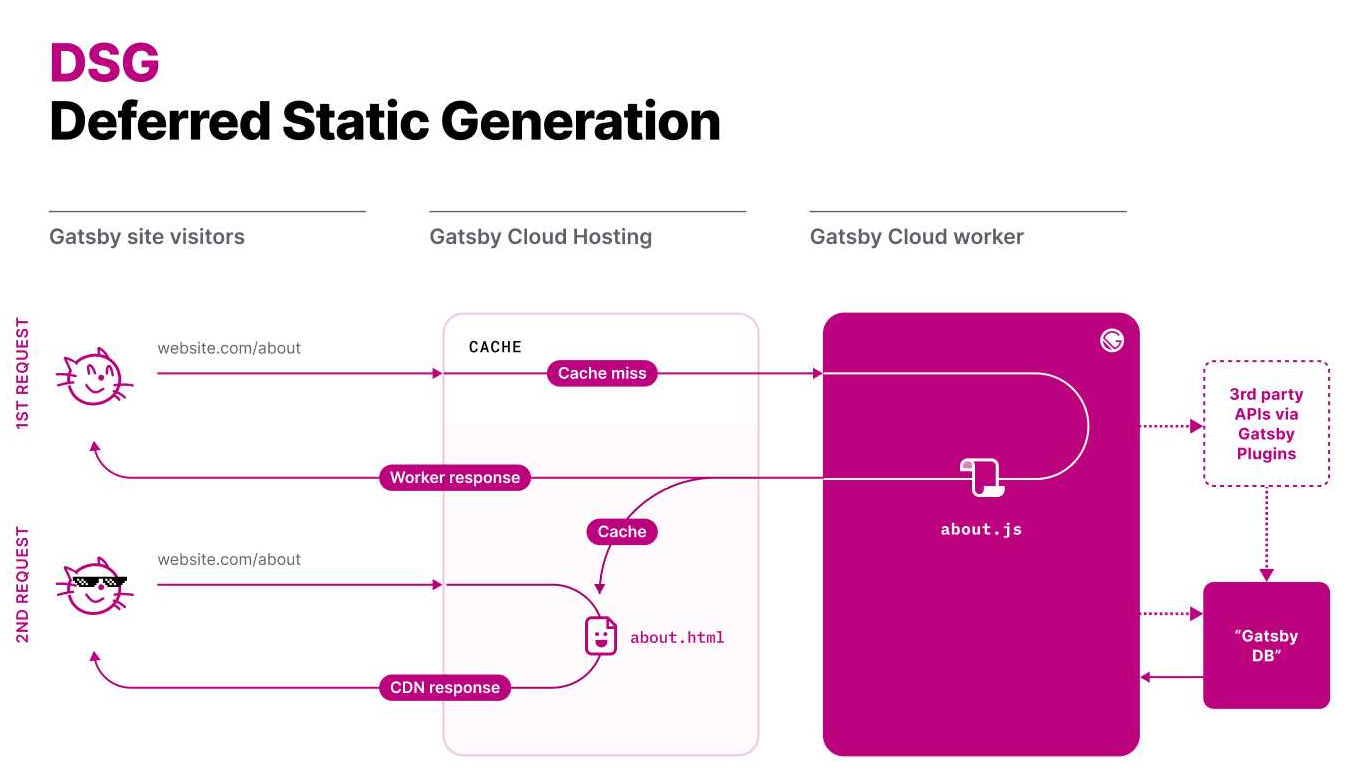
\includegraphics[width=0.9\textwidth]{media/deferred_static_generation_dsg.png}
  \legend{Fonte: \cite{gatsby2023}}
  \label{fig:deferred_dsg}
\end{figure}

Na \autoref{fig:deferred_dsg}, observa-se que, ao acessar uma página como \texttt{/about} pela primeira vez, ocorre um \textit{cache miss}, e um \textit{worker} do Gatsby é acionado para gerar o arquivo \texttt{about.html} a partir do componente correspondente (\texttt{about.js}). Esse conteúdo pode incluir dados extraídos de plugins, \textit{APIs} de terceiros ou do próprio \textit{Gatsby DB}. Após o processamento, a resposta é enviada ao usuário e armazenada em cache. Requisições futuras à mesma rota são atendidas diretamente pela CDN, com desempenho semelhante ao de páginas \acrshort{ssg}.

Segundo \citeonline{locofy2024}, a estratégia do \acrshort{dsg} é especialmente útil para projetos com milhares de páginas cujo acesso é desigual. Exemplos incluem catálogos de produtos legados, páginas de arquivos antigos ou conteúdos gerados a partir de sistemas CMS.

A seguir, um exemplo de configuração de uma rota com \acrshort{dsg} em Gatsby:

\begin{codigo}[H]
  \begin{lstlisting}[language=JavaScript]
// gatsby-node.js
exports.createPages = async ({ actions }) => {
  const { createPage } = actions
  createPage({
    path: `/produto/exemplo`,
    component: require.resolve(`./src/templates/produto.js`),
    context: { id: `produto-exemplo` },
    defer: true, // ativa DSG
  })
}
  \end{lstlisting}
  \caption{Exemplo de definição de página DSG no Gatsby}
  \label{cod:dsg_example}
\end{codigo}

Assim como o \acrshort{isr}, o \acrshort{dsg} busca combinar desempenho, escalabilidade e atualizações eficientes. No entanto, sua particularidade está em adiar completamente o custo da renderização até o momento da primeira requisição, tornando-o ideal em contextos onde o tempo de build precisa ser otimizado sem prejudicar a entrega do conteúdo a longo prazo.

















\section{Métricas e Ferramentas de Análise de Desempenho}
\label{sec:metricas-e-ferramentas}
A avaliação de desempenho em aplicações web modernas é um pilar fundamental para garantir a qualidade da experiência do usuário e o sucesso de um projeto. A análise vai muito além do simples tempo de carregamento total, abrangendo a percepção de velocidade, a capacidade de resposta a interações e a estabilidade visual da interface. Para quantificar esses aspectos de forma padronizada e acionável, o ecossistema de desenvolvimento web dispõe de um conjunto robusto de métricas e ferramentas, que foram essenciais para a coleta de dados e a análise comparativa deste trabalho.

\subsection{Ferramentas de Análise de Mercado}
\label{subsec:ferramentas-analise}
Existem diversas ferramentas consolidadas para a análise de performance web. Soluções como o \textbf{PageSpeed Insights}, \textbf{GTmetrix} e \textbf{WebPageTest} oferecem diagnósticos detalhados sobre a velocidade de carregamento e a experiência do usuário, simulando diferentes condições de rede, dispositivos e localizações geográficas \cite{webabsoluta_ferramentas}. Enquanto o PageSpeed Insights se destaca por integrar dados de campo (do Chrome User Experience Report) e de laboratório, o GTmetrix é conhecido por seus relatórios detalhados com gráficos em cascata (\textit{waterfall charts}) que ajudam a identificar gargalos no carregamento de recursos \cite{gtmetrix_vitals}. O WebPageTest, por sua vez, oferece uma flexibilidade granular nos testes. Para este trabalho, a análise foi centrada em duas iniciativas principais do Google: o Lighthouse e, principalmente, os Core Web Vitals.

\subsection{Google Lighthouse}
\label{subsec:google-lighthouse}
O \textbf{Google Lighthouse} é uma ferramenta de auditoria automatizada e de código aberto, integrada às ferramentas de desenvolvedor do Google Chrome. Ele é projetado para analisar a qualidade de páginas web em cinco categorias principais: Performance, Acessibilidade, Boas Práticas, SEO e \textit{Progressive Web App} (PWA). Ao final da análise, o Lighthouse gera um relatório com pontuações de 0 a 100 para cada categoria e apresenta um conjunto de oportunidades e diagnósticos acionáveis. No contexto deste estudo, o Lighthouse foi utilizado como uma ferramenta de apoio diagnóstico em ambiente de laboratório, essencial para identificar gargalos de renderização, analisar o tempo de bloqueio da \textit{thread} principal (\textit{Total Blocking Time}) e validar aspectos técnicos de SEO e acessibilidade das aplicações desenvolvidas.

\subsection{Core Web Vitals}
\label{subsec:core-web-vitals}
O pilar da coleta de dados empíricos deste trabalho foi o conjunto de métricas conhecido como \textbf{Core Web Vitals}. Proposto pelo Google, este subconjunto dos Web Vitals foi projetado para medir a experiência do usuário no mundo real (\textit{field data}), focando em três aspectos que impactam diretamente a percepção do usuário: velocidade de carregamento, interatividade e estabilidade visual \cite{osmani2025}. A importância dessas métricas é reforçada pelo fato de serem um fator de ranqueamento nos resultados de busca do Google \cite{google_cwv_search}.

\subsubsection{Principais Métricas do Web Vitals}
As métricas a seguir, que compõem os Core Web Vitals atuais, foram essenciais para a análise comparativa:
\begin{description}
    \item[\textbf{LCP (\acrfull{lcp})}] Mede o tempo, em segundos, desde o início do carregamento da página até a renderização do maior elemento de conteúdo (imagem ou bloco de texto) visível na tela. É a principal métrica para a percepção de velocidade de carregamento.
    \item[\textbf{INP (\acrfull{inp})}] Avalia a latência de todas as interações do usuário (cliques, toques e digitação) com a página, medindo a capacidade de resposta geral da aplicação. Um baixo INP indica que a página responde rapidamente às ações do usuário.
    \item[\textbf{CLS (\acrfull{cls})}] Quantifica a instabilidade visual da página. Mede a soma de todas as mudanças inesperadas de layout que ocorrem durante o carregamento, garantindo que os elementos não "pulem" na tela e frustrem a interação do usuário.
\end{description}

\subsubsection{Métricas Complementares}
Além dos Core Web Vitals, outras métricas foram observadas para fornecer um diagnóstico mais completo do processo de carregamento:
\begin{description}
    \item[\textbf{TTFB (\acrfull{ttfb})}] Indica a responsividade do servidor. Mede o tempo entre a requisição de um recurso e o momento em que o primeiro byte da resposta chega ao navegador. É um indicador crucial da saúde do \textit{backend}.
    \item[\textbf{FCP (\acrfull{fcp})}] Marca o tempo em que o primeiro conteúdo do \acrshort{dom} (texto, imagem, etc.) é renderizado na tela, dando ao usuário o primeiro feedback visual de que a página está carregando.
    \item[\textbf{TBT (Total Blocking Time)}] Medido em ambiente de laboratório (via Lighthouse), soma o tempo em que a \textit{thread} principal ficou bloqueada por tarefas longas, impedindo a resposta a interações do usuário. É um bom proxy para a métrica de campo INP.
\end{description}
O domínio e a correta interpretação dessas métricas foram fundamentais para a análise comparativa entre as arquiteturas CSR e SSR, permitindo uma compreensão aprofundada do desempenho percebido pelo usuário e servindo como base para as conclusões técnicas apresentadas neste estudo.






























\section{Frameworks Web}
\label{sec:frameworks-web}

O uso de bibliotecas e frameworks no desenvolvimento web moderno proporciona ganhos significativos de produtividade, desempenho e organização de código. Eles abstraem operações complexas e oferecem estruturas padronizadas para construção de aplicações escaláveis. A escolha da ferramenta está diretamente relacionada à abordagem de renderização adotada, seja no lado do cliente (\acrshort{csr}) ou do servidor (\acrshort{ssr}).

\subsection{Bibliotecas JavaScript}
\label{subsec:bibliotecas-js}

Bibliotecas JavaScript são conjuntos de funcionalidades reutilizáveis que fornecem recursos específicos para o desenvolvimento de aplicações web. Elas diferem dos frameworks por não imporem uma estrutura rígida, oferecendo maior flexibilidade ao desenvolvedor. A seguir, são apresentadas algumas das bibliotecas mais relevantes no contexto de renderização do lado do cliente (\acrshort{csr}):


\begin{itemize}
  \item \textbf{React:} Desenvolvida pelo Facebook, React é uma biblioteca declarativa focada na construção de interfaces de usuário por meio de componentes reutilizáveis. Seu uso do \textit{virtual DOM} permite renderizações mais eficientes, tornando-a ideal para aplicações interativas com alto desempenho. Apesar de ser comumente chamada de framework, React atua apenas na camada de visualização, exigindo bibliotecas complementares para roteamento e gerenciamento de estado~\cite{react2025}.

  \item \textbf{jQuery:} Uma das bibliotecas mais populares da era inicial do JavaScript moderno, jQuery simplifica tarefas comuns como manipulação do DOM, tratamento de eventos e requisições AJAX. Embora sua popularidade tenha diminuído com o surgimento de bibliotecas mais modernas e frameworks reativos, ela ainda é amplamente utilizada em sistemas legados e aplicações de menor complexidade~\cite{jquery2023}.

  \item \textbf{Alpine.js:} Alpine.js é uma biblioteca leve e reativa voltada para a manipulação de componentes diretamente no HTML, com uma sintaxe declarativa inspirada em Vue.js. Ela é particularmente útil para adicionar interatividade a páginas estáticas ou aplicações simples, sendo uma alternativa eficiente em cenários onde o uso de bibliotecas maiores seria excessivo~\cite{alpinejs2023}.
\end{itemize}

\subsection{Frameworks para CSR}
\label{subsec:frameworks-csr}

No modelo \acrshort{csr}, a renderização da interface é realizada diretamente no navegador do usuário, após o carregamento dos arquivos JavaScript. Frameworks como os listados a seguir são amplamente utilizados para implementar essa abordagem:

\begin{itemize}
    \item \textbf{Vue.js}: framework progressivo para construção de interfaces web interativas. Seu foco está na camada de visualização, com curva de aprendizado acessível e estrutura modular~\cite{vue2025}.
    
    \item \textbf{Angular}: framework completo mantido pelo Google, baseado em TypeScript, que oferece arquitetura robusta e recursos integrados como injeção de dependência e roteamento~\cite{angular2025}.
    
    \item \textbf{Svelte}: framework que realiza a compilação dos componentes no momento do build, eliminando a necessidade de um \textit{virtual DOM}, o que reduz o tempo de carregamento e o uso de recursos do navegador~\cite{svelte2025}.
\end{itemize}

Esses frameworks tornam o desenvolvimento com \acrshort{csr} mais eficiente e sustentável, proporcionando experiências ricas ao usuário com foco em interatividade e responsividade.

\subsection{Meta-frameworks para SSR}
\label{subsec:frameworks-ssr}

Para aplicações com foco em renderização no lado do servidor, os \emph{meta-frameworks} oferecem soluções completas, otimizando tanto o desempenho inicial quanto a indexabilidade em mecanismos de busca. Eles operam sobre frameworks tradicionais (como Vue ou Svelte) ou bibliotecas (como React), incorporando funcionalidades essenciais como roteamento, pré-renderização, recuperação de dados e \textit{hydration}.

\begin{itemize}
    \item \textbf{Next.js}: baseado em React, fornece recursos para \acrshort{ssr}, geração de sites estáticos e suporte a APIs integradas~\cite{nextjs2024}.
    
    \item \textbf{Nuxt.js}: extensão do Vue.js que oferece SSR, geração estática e arquitetura modular~\cite{nuxtjs2024}.
    
    \item \textbf{SvelteKit}: baseado em Svelte, permite renderização no servidor e no cliente, com foco em simplicidade e desempenho~\cite{sveltekit2024}.
    
    \item \textbf{Angular Universal}: solução oficial para SSR em Angular, melhora a indexação e o tempo de carregamento inicial~\cite{angularuniversal2024}.
    
    \item \textbf{Remix}: framework full-stack para React que adota um modelo de dados centrado em carregadores e ações~\cite{remix2024}.
    
    \item \textbf{Astro}: framework moderno que carrega apenas o JavaScript necessário, permitindo uso híbrido de componentes React, Vue, Svelte e outros~\cite{astro2024}.
    
    \item \textbf{Qwik}: introduz o conceito de aplicações \textit{resumíveis}, com SSR e carregamento progressivo de interatividade~\cite{qwik2024}.
\end{itemize}

Esses meta-frameworks são especialmente indicados para aplicações que priorizam SEO, acessibilidade e desempenho no primeiro carregamento, como páginas institucionais, lojas virtuais e blogs.

\subsection{Comparativo entre Frameworks CSR e SSR}
\label{subsec:comparativo-frameworks}

\begin{table}[H]
\centering
\caption{Comparação entre frameworks para CSR e SSR}
\label{tab:comparativo-frameworks}
\begin{tabular}{|p{3cm}|p{5.5cm}|p{5.5cm}|}
\hline
\textbf{Critério} & \textbf{Frameworks CSR (Vue, Angular, Svelte)} & \textbf{Meta-frameworks SSR (Next.js, Nuxt, SvelteKit, etc.)} \\
\hline
\textbf{Renderização Inicial} & O conteúdo é montado no navegador após o carregamento do JavaScript & O conteúdo é gerado no servidor e entregue já renderizado ao navegador \\
\hline
\textbf{Tempo de Carregamento} & Maior tempo de carregamento inicial (dependente do JS) & Melhor desempenho no carregamento inicial (TTFB menor) \\
\hline
\textbf{SEO} & Pode ser limitado, pois bots podem não processar JavaScript adequadamente & Excelente, já que o HTML completo está disponível para rastreadores \\
\hline
\textbf{Interatividade} & Alta, com foco em aplicações ricas e dinâmicas & Boa, com necessidade de \textit{hydration} após o carregamento \\
\hline
\textbf{Complexidade de Infraestrutura} & Menor, geralmente servido por CDNs e arquivos estáticos & Maior, exige servidores para processar cada requisição \\
\hline
\textbf{Casos de Uso Ideais} & SPAs, dashboards, aplicações com muitas interações em tempo real & Landing pages, blogs, e-commerces, sites que dependem de SEO \\
\hline
\end{tabular}
\end{table}


% \subsection{Modelos de Arquitetura Web}
% \label{subsec:modelos-arq-web}
% Os modelos arquiteturais variam conforme os requisitos de escalabilidade, manutenção e desempenho:

% \begin{itemize}
%     \item \textbf{Arquitetura Monolítica}: Um único projeto concentra \textit{frontend} e \textit{backend}, frequentemente usando \acrshort{ssr}. Possui inicialização simples, mas pode tornar-se complexo de manter e escalar.
%     \item \textbf{Microserviços}: Divide a aplicação em múltiplos serviços independentes. Cada serviço pode escolher a melhor abordagem de renderização (SSR ou CSR), facilitando a escalabilidade seletiva.
%     \item \textbf{Serverless}: As funções são executadas sob demanda em plataformas de nuvem, onde a renderização pode ocorrer tanto no servidor (funções que retornam HTML) quanto no cliente (ao entregar apenas APIs).
% \end{itemize}

% \subsection{Ferramentas e \textit{Frameworks}}
% \label{subsec:ferramentas-frameworks}
% O ecossistema de desenvolvimento web oferece diversas ferramentas que simplificam \acrshort{ssr} e \acrshort{csr}:

% \begin{itemize}
%     \item \textbf{\acrshort{ssr}}: \textit{Next.js} (React), \textit{Nuxt.js} (Vue), \textit{SvelteKit} (Svelte), entre outros.
%     \item \textbf{\acrshort{csr}}: React, Vue.js, Angular e muitas bibliotecas voltadas para \textit{Single Page Applications} (SPA).
% \end{itemize}


% \section{Infraestrutura de Serviço Web}
% \label{sec:infraestrutura-web}

% A decisão por \acrshort{ssr} ou \acrshort{csr} influencia diretamente a infraestrutura necessária:

% \begin{itemize}
%     \item \textbf{Servidores e Processamento}: Em \acrshort{ssr}, o servidor gera páginas dinamicamente, aumentando a carga de CPU. Já em \acrshort{csr}, o servidor atua mais como um provedor de arquivos estáticos e APIs.
%     \item \textbf{\english{Content Delivery Networks} (CDNs)}: Tanto para SSR quanto para CSR, uma CDN pode melhorar a distribuição de arquivos estáticos (HTML, CSS, JavaScript, imagens) e reduzir a latência.
%     \item \textbf{Escalabilidade}: Aplicações com alto número de requisições precisam de estratégias adequadas para lidar com picos de acesso. Em \acrshort{ssr}, muitas requisições simultâneas podem sobrecarregar o servidor; em \acrshort{csr}, o foco está em serviços de dados e na entrega eficiente de arquivos iniciais.
% \end{itemize}

% \textbf{Segurança} também se faz presente em ambas as abordagens. Boas práticas incluem:
% \begin{itemize}
%     \item Uso de \textbf{HTTPS} para proteger a comunicação.
%     \item Implementação de \textbf{CORS} (Cross-Origin Resource Sharing) quando necessário.
%     \item Tratamento de \textbf{tokens de sessão/autenticação} com cuidado para evitar vazamento de dados.
% \end{itemize}

% ---

\section{Experiência do Usuário}
\label{sec:ux}
A \acrfull{ux} é um aspecto crítico no desenvolvimento de aplicações web, influenciando diretamente a satisfação e a eficácia da interação do usuário com o sistema \cite{atori2023}. Para alcançar uma \acrshort{ux} satisfatória, a escolha entre \acrshort{csr} e \acrshort{ssr} deve considerar fatores como: {\acrshort{seo}}, velocidade de carregamento, interatividade e acessibilidade.
Conforme \citeonline{atori2024}, a \acrshort{ux} vai além da interface gráfica, englobando toda a jornada do usuário desde a navegação até a conclusão de tarefas. 

\subsection{\english{Search Engine Optimization} (SEO)}
\label{sec:seo}

O \acrfull{seo} consiste em um conjunto integrado de práticas de otimização, tanto no aspecto técnico quanto no de conteúdo, com três objetivos principais: maximizar a visibilidade orgânica nos mecanismos de busca, posicionar estrategicamente páginas-chave e garantir uma experiência de usuário qualificada durante o processo de busca. Essas práticas são essenciais para garantir que o conteúdo de um site seja facilmente encontrado e indexado pelos motores de busca, aumentando a probabilidade de atrair visitantes qualificados. Entre os fatores mais conhecidos, destaca-se a velocidade de carregamento da página, que impacta diretamente a experiência do usuário e a classificação nos resultados de busca \cite{conor2022}.
\begin{figure}[H]
    \centering
    \caption{Tempo de Rastreamento e Posicionamento da Página}
    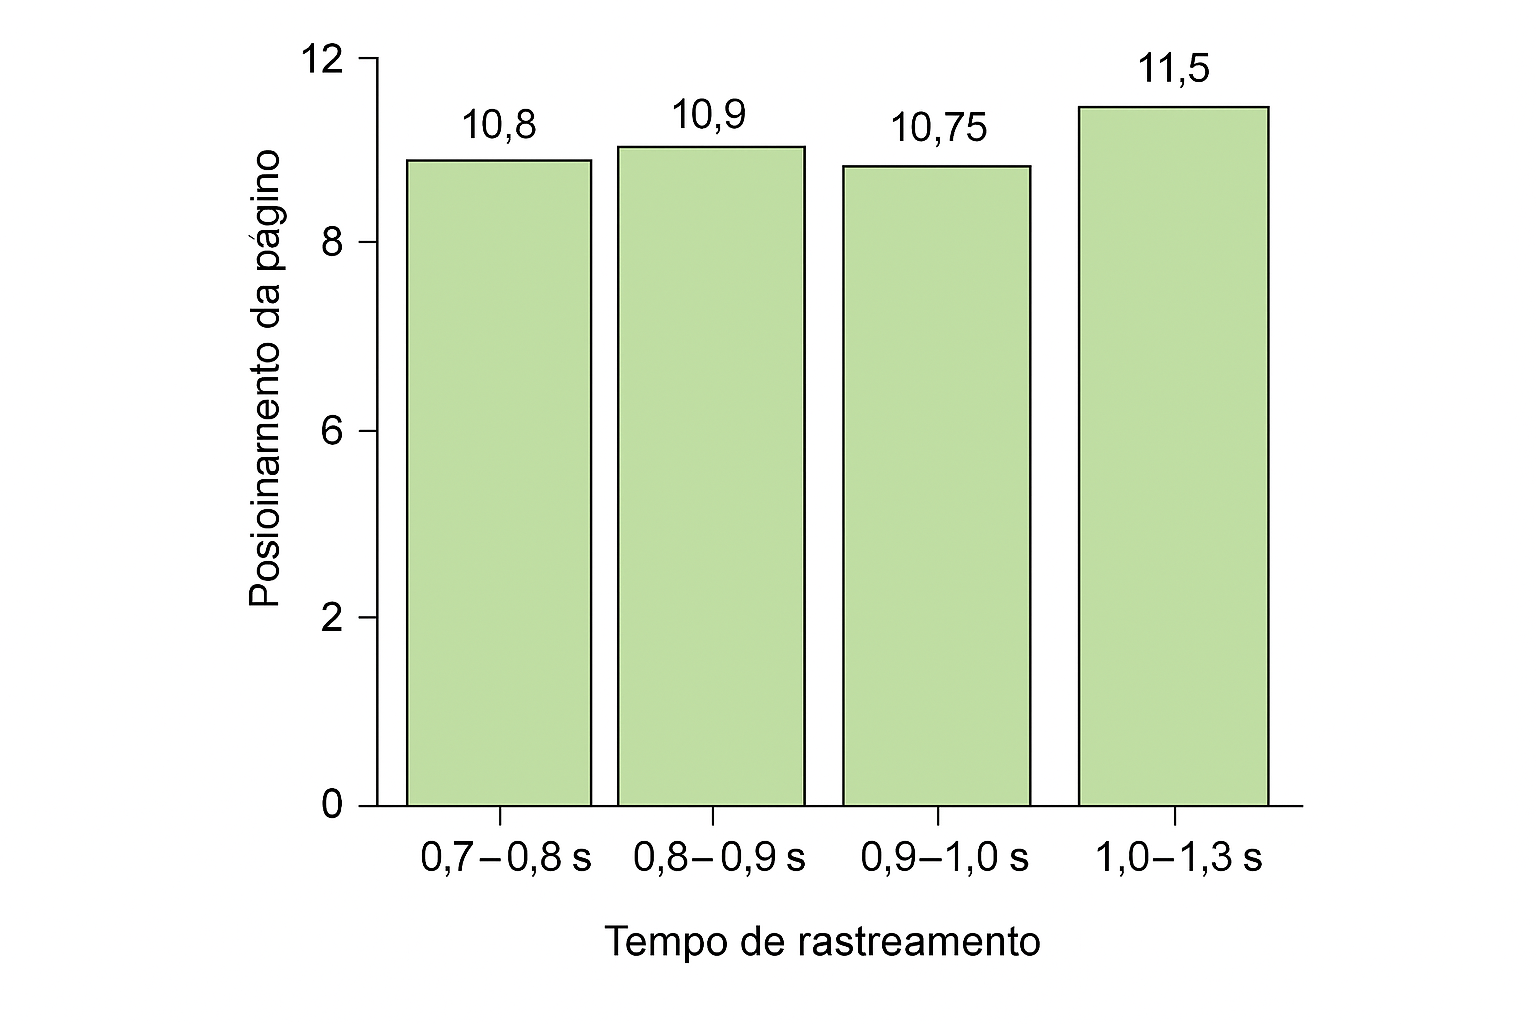
\includegraphics[width=0.6\textwidth]{media/rank_crawl_and_page_rank.png}
    \legend{Fonte: \cite{webPerformance}(adaptado)}
    \label{fig:rank_crawl_and_page_rank}
\end{figure}

A \autoref{fig:rank_crawl_and_page_rank} ilustra a relação entre o tempo de rastreamento e o posicionamento da página. O tempo de rastreamento refere-se ao tempo que os mecanismos de busca levam para acessar e indexar uma página. Quanto mais rápido o tempo de rastreamento, maior a probabilidade de a página ser indexada rapidamente e, consequentemente, melhor seu posicionamento nos resultados de busca. Isso destaca a importância de otimizar o desempenho do site para garantir uma boa classificação nos motores de busca.

\subsection{\english{Velocidade de carregamento}}
\label{sec:velocidade da página}

A velocidade de carregamento de uma página refere-se ao tempo necessário para que todo o seu conteúdo esteja visível e interativo no navegador, desde a solicitação inicial do usuário. Esse tempo pode ser influenciado por diversos fatores, como o tamanho dos arquivos, a complexidade do conteúdo, a qualidade da conexão com a internet e o desempenho do servidor \cite{shopify2024}.

Esse fator é determinante tanto para a \acrshort{ux} quanto para o \acrshort{seo}. Páginas que carregam rapidamente tendem a apresentar menores taxas de rejeição e melhores resultados em métricas de conversão. Além disso, o \acrshort{seo} utiliza a velocidade de carregamento como um dos critérios de ranqueamento nos mecanismos de busca \cite{conor2022}.

De acordo com \citeonline{google}, quanto mais rápido um site carregar, melhor tende a ser a experiência do usuário. Sites lentos comprometem a navegação e reduzem o tempo de permanência, afetando negativamente o engajamento.

A percepção de desempenho muitas vezes chamada de \emph{velocidade percebida} também é um fator crucial para a usabilidade e pode ser tão relevante quanto o tempo de carregamento real. Nesse sentido, a escolha entre \acrshort{ssr} e \acrshort{csr} influencia diretamente essa percepção. O \acrshort{ssr} geralmente proporciona carregamento inicial mais rápido, pois o conteúdo é renderizado no servidor e entregue ao navegador já pronto para exibição. Isso permite que os usuários visualizem o conteúdo principal imediatamente, mesmo que outros recursos ainda estejam sendo carregados \cite{atori2024}.

Por outro lado, no \acrshort{csr}, o navegador precisa baixar, interpretar e executar o JavaScript antes de renderizar qualquer conteúdo. Isso pode resultar em uma exibição inicial em branco ou em telas de carregamento, o que compromete a percepção de desempenho especialmente em conexões lentas ou dispositivos com menor capacidade de processamento \cite{pixelfree2023}.


\subsection{Interatividade}
\label{subsec:interatividade}

A interatividade é um fator decisivo na experiência do usuário em aplicações web modernas, pois determina a forma como os usuários percebem a continuidade e a capacidade de resposta durante a navegação. Nas aplicações que utilizam \acrshort{csr}, o código JavaScript é executado diretamente no navegador, permitindo respostas imediatas a interações como cliques, preenchimento de formulários ou navegação entre páginas internas. Essa abordagem possibilita transições de página mais suaves e experiências semelhantes às de aplicativos nativos, sem a necessidade de recarregamentos completos \cite{pixelfree2023}.

Segundo \citeonline{atori2024}, a renderização no lado do cliente favorece experiências altamente dinâmicas, oferecendo um nível elevado de controle sobre os elementos da interface. Em contrapartida, o \acrshort{ssr}, embora proporcione carregamento inicial mais rápido e visibilidade imediata do conteúdo, apresenta limitações em termos de interatividade. Alterações na interface em aplicações \acrshort{ssr} geralmente demandam comunicações adicionais com o servidor, o que pode comprometer a continuidade da experiência do usuário \cite{atori2024, splunk2023}.

Para mitigar essas limitações, abordagens híbridas têm sido amplamente adotadas. Nelas, o conteúdo é inicialmente renderizado no servidor e, posteriormente, reativado no cliente com JavaScript, em uma estratégia conhecida como \emph{hydration} \cite{splunk2023}. Essa técnica busca aliar os benefícios de desempenho e \acrshort{seo} do \acrshort{ssr} com a interatividade aprimorada do \acrshort{csr}.


\subsection{Acessibilidade}
\label{subsec:acessibilidade}

A acessibilidade em aplicações web refere-se à capacidade de tornar conteúdos e funcionalidades utilizáveis por pessoas com deficiência, como visual, auditiva, motora ou cognitiva. É um princípio essencial para garantir a equidade no acesso à informação e à interação digital. De acordo com \cite{pixelfree2023access}, acessibilidade diz respeito a assegurar que todos, independentemente de suas habilidades, possam acessar e interagir com o conteúdo da web. Para pessoas com deficiência, isso pode significar o uso de leitores de tela, navegação por teclado ou a dependência de outras tecnologias assistivas.

As abordagens de renderização, como \acrshort{csr} e \acrshort{ssr}, impactam diretamente a acessibilidade, especialmente na compatibilidade com essas tecnologias. Em aplicações que utilizam \acrshort{csr}, o conteúdo geralmente é carregado de forma assíncrona após a execução do JavaScript, o que pode dificultar a leitura imediata por leitores de tela que dependem de uma estrutura HTML previamente carregada para interpretar a página corretamente \cite{pixelfree2023access}. Já no \acrshort{ssr}, o conteúdo é entregue completamente no carregamento inicial, facilitando a interpretação por essas ferramentas e proporcionando uma experiência mais estável para usuários com deficiência visual \cite{atori2024}.

Além disso, em contextos com atualizações dinâmicas de conteúdo como ocorre em SPAs com \acrshort{csr} é necessário adotar práticas específicas para garantir a acessibilidade, como gerenciamento de foco, uso de alertas ARIA e atualização de leitores de tela após mudanças no DOM. Essas medidas são fundamentais para que as mudanças de visualização sejam percebidas corretamente por tecnologias assistivas, uma vez que alterações no DOM nem sempre são reconhecidas automaticamente por leitores de tela. O envio de foco a elementos interativos ou o uso de regiões ARIA ao vivo são técnicas recomendadas para anunciar mudanças de estado ao usuário \cite{sutton2018}.

Assim, embora o \acrshort{ssr} ofereça uma base naturalmente mais acessível, ambas as abordagens podem ser igualmente inclusivas quando aplicadas com atenção às diretrizes e boas práticas de acessibilidade.



\section{Ferramentas Modernas para Prototipação e Interfaces}
\label{sec:ferramentas-modernas}

Nesta seção são apresentadas duas ferramentas inovadoras utilizadas para acelerar o desenvolvimento frontend: a plataforma \textbf{v0} e a biblioteca de componentes \textbf{shadcn/ui}. Ambas representam abordagens modernas para construção de interfaces dinâmicas, acessíveis e escaláveis.

\subsection{v0}
\label{subsec:v0}

A \textbf{v0} é uma plataforma assistida por Inteligência Artificial projetada para transformar descrições em linguagem natural em aplicações web funcionais. A partir de prompts descritivos, a ferramenta gera código utilizando tecnologias modernas como React, Next.js e Tailwind CSS, permitindo prototipação rápida e iteração sobre interfaces \cite{v0_docs}. O fluxo básico inclui: escrever a ideia em texto, gerar a interface automaticamente, revisar e ajustar os elementos e exportar o código para integração no projeto.

\subsection{shadcn/ui}
\label{subsec:shadcn}

O \textbf{shadcn/ui} é uma biblioteca de componentes open source baseada em Radix UI e estilizada com Tailwind CSS. Ao contrário de bibliotecas tradicionais, os componentes do \textbf{shadcn/ui} são copiados diretamente para o projeto, oferecendo ao desenvolvedor total controle sobre o código e possibilitando personalizações profundas \cite{shadcn_docs}. Essa abordagem favorece flexibilidade e consistência visual no desenvolvimento de aplicações modernas.

\subsection{Integração entre v0 e shadcn/ui}
\label{subsec:integracao-v0-shadcn}

A integração entre \textbf{v0} e \textbf{shadcn/ui} proporciona uma experiência otimizada para geração de interfaces. Ao utilizar a plataforma \textbf{v0}, os componentes gerados são construídos com base na arquitetura do \textbf{shadcn/ui}, incluindo as práticas recomendadas de acessibilidade e estilização com Tailwind CSS \cite{v0_docs, shadcn_docs}. Essa integração permite que desenvolvedores iniciem com protótipos gerados automaticamente e, em seguida, façam ajustes diretamente no código dos componentes, mantendo um alto grau de personalização e performance. Além disso, ela favorece o uso de estratégias modernas como \acrshort{ssr} e \acrshort{csr}, oferecendo compatibilidade com frameworks como Next.js e Vite.




\section{Processo de Desenvolvimento e Controle de Gestão de Software}
\label{sec:git-github}

O desenvolvimento de aplicações web modernas exige práticas que garantam organização, rastreabilidade e colaboração eficiente entre desenvolvedores. Nesse contexto, ferramentas de controle de versão como o \textbf{Git} e plataformas de hospedagem como o \textbf{GitHub} são fundamentais para o gerenciamento do ciclo de vida do software \cite{github_official}.

\subsection{Git}
\label{subsec:git}

O \textbf{Git} é um sistema de controle de versão distribuído criado por Linus Torvalds em 2005 com o objetivo de gerenciar projetos de forma rápida e eficiente, independentemente do tamanho ou complexidade \cite{chacon_git}. Ele permite que múltiplos desenvolvedores trabalhem simultaneamente em um projeto, mantendo o histórico de alterações de forma segura e auditável.

Entre os conceitos fundamentais do Git, destacam-se:

\begin{itemize}
\item \textbf{Repositório (\textit{Repository}):} Estrutura que armazena o histórico completo do projeto, incluindo arquivos, diretórios e suas versões ao longo do tempo.
\item \textbf{Commits:} Registros de alterações no projeto. Cada commit possui um identificador único (hash) e uma mensagem descritiva \cite{chacon_git}.
\item \textbf{Branches:} Ramificações independentes do repositório que permitem o desenvolvimento paralelo de funcionalidades, correções ou experimentos sem impactar o código principal.
\item \textbf{Merge:} Integração de alterações realizadas em diferentes branches.
\item \textbf{Clone e Pull:} Operações que permitem obter uma cópia local do repositório e sincronizar com atualizações remotas.
\end{itemize}

O modelo distribuído do Git permite que cada colaborador mantenha uma cópia completa do repositório em sua máquina local, o que garante maior resiliência e independência em relação ao servidor central \cite{chacon_git}.

\subsection{GitHub}
\label{subsec:github}

O \textbf{GitHub} é uma plataforma de hospedagem de código baseada em Git, que amplia suas funcionalidades com recursos colaborativos e integração contínua \cite{github_official}. Fundada em 2008, a plataforma popularizou-se como um ambiente de colaboração para projetos de software de código aberto e privado.

Além de hospedar repositórios Git, o GitHub oferece funcionalidades como:

\begin{itemize}
\item \textbf{Issues:} Ferramenta para rastreamento de tarefas, bugs e melhorias \cite{github_official}.
\item \textbf{Pull Requests (PR):} Fluxo de revisão e integração de código, permitindo que contribuições sejam analisadas antes de serem incorporadas ao branch principal.
\item \textbf{Actions:} Automatização de processos com integração contínua (CI) e entrega contínua (CD).
\item \textbf{Wikis e Documentação:} Área para criação de páginas informativas sobre o projeto.
\end{itemize}

\subsection{GitHub Projects}
\label{subsec:github-projects}

O \textbf{GitHub Projects} é uma funcionalidade integrada à plataforma que possibilita o gerenciamento de projetos utilizando quadros visuais baseados em metodologias ágeis, como Kanban e Scrum \cite{github_projects}. Essa ferramenta permite organizar tarefas, acompanhar o progresso e priorizar demandas de maneira colaborativa.

Entre os recursos oferecidos pelo GitHub Projects, destacam-se:

\begin{itemize}
\item \textbf{Quadros Kanban:} Visualização de tarefas em colunas (como \textit{To Do}, \textit{In Progress} e \textit{Done}), facilitando o acompanhamento do fluxo de trabalho.
\item \textbf{Automação:} Regras automáticas que movem cartões entre colunas com base em eventos, como o fechamento de issues ou merge de pull requests \cite{github_projects}.
\item \textbf{Customização:} Campos personalizados e filtros para adaptar o quadro às necessidades do projeto.
\item \textbf{Integração com Issues e Pull Requests:} Possibilidade de vincular tarefas diretamente ao código, permitindo rastreabilidade completa entre planejamento e implementação.
\end{itemize}






\section{News API}
\label{sec:news-api}

A \textbf{News API} é uma interface de programação que disponibiliza fluxos de notícias e artigos de forma estruturada, permitindo o acesso a conteúdos de mais de 150\,000 fontes jornalísticas ao redor do mundo. Seu propósito é fornecer informações publicadas em tempo real, facilitando o desenvolvimento de soluções de agregação, análise e visualização de notícias \cite{newsapi_docs}.

\subsection{Escopo e cobertura}
A plataforma oferece dois principais tipos de consulta: 

\begin{itemize}
    \item \textbf{Busca por artigos (\texttt{/everything}):} permite pesquisar notícias com base em termos, operadores booleanos, intervalos de datas, domínios específicos e critérios de ordenação, como relevância, popularidade ou data de publicação \cite{newsapi_docs}.
    \item \textbf{Manchetes principais (\texttt{/top-headlines}):} retorna as notícias mais recentes, com filtros por país, categoria jornalística e fontes específicas.
\end{itemize}

Além disso, a \textbf{News API} disponibiliza o endpoint \texttt{/sources}, que fornece metadados sobre os veículos indexados, como nome, idioma, categoria e URL oficial.

\subsection{Autenticação e formato de resposta}
Para utilizar os endpoints, é necessário um \acrshort{api} key, que autentica as requisições e controla o uso da plataforma. As respostas são retornadas no formato \acrshort{json}, contendo campos como \texttt{status}, \texttt{totalResults} e uma lista de objetos \texttt{articles}, com atributos como título, autor, descrição, \acrshort{url} e data de publicação \cite{newsapi_docs}.

\subsection{Funcionalidade e integração}
A \textbf{News API} suporta buscas avançadas com:

\begin{itemize}
    \item termos exatos ou operadores lógicos (\texttt{AND}, \texttt{OR}, \texttt{NOT});
    \item filtros por idioma, domínios específicos e intervalos de datas (\texttt{from}, \texttt{to});
    \item paginação e controle de volume de resultados, com limite máximo de 100 artigos por página.
\end{itemize}

Essas características permitem integração tanto em aplicações com \acrshort{csr}, que realizam chamadas diretamente do navegador após o carregamento, quanto em soluções com \acrshort{ssr}, onde as requisições são feitas na camada servidor, possibilitando que o conteúdo seja renderizado previamente antes de ser entregue ao cliente.






\section{Contêineres e Docker}
\label{cap:docker}

Este capítulo apresenta os conceitos fundamentais de contêineres e da plataforma \textbf{Docker}, incluindo sua arquitetura, objetos principais (imagens, camadas, contêineres, redes e volumes) e o processo de construção de imagens por meio do \textbf{Dockerfile}. Também são discutidas boas práticas de construção (multi-stage builds, cache, uso de \texttt{.dockerignore} e \textit{secrets}) e a integração com o estudo comparativo \acrshort{csr} x \acrshort{ssr}. \cite{docker_overview,dockerfile_ref} 

\subsection{Visão Geral da Plataforma Docker}
\label{sec:docker-overview}

O \textbf{Docker} é uma plataforma de código aberto que permite empacotar, distribuir e executar aplicações em ambientes isolados chamados \textbf{contêineres}. Esses contêineres são leves, portáveis e contêm tudo o que é necessário para executar a aplicação (bibliotecas, dependências e configurações), reduzindo a variação entre ambientes e acelerando ciclos de \acrshort{ci}/\acrshort{cd} \cite{docker_overview}. 

\subsection{Arquitetura: cliente–servidor}
\label{subsec:docker-arquitetura}

A arquitetura do Docker segue o modelo cliente–servidor: o \textbf{cliente} (\texttt{docker}) envia comandos para o \textbf{daemon} (\texttt{dockerd}), que executa as operações de \textit{build}, execução e distribuição de imagens e contêineres. A comunicação ocorre via \acrshort{api} do Docker, por \textit{Unix sockets} ou interface de rede. O \textbf{Docker Desktop} integra esses componentes e ferramentas correlatas (Compose, Kubernetes opcional, etc.) \cite{docker_overview}. 

\begin{figure}[H]
  \centering
  \caption{Arquitetura simplificada do Docker (cliente, daemon, registries e objetos).}
  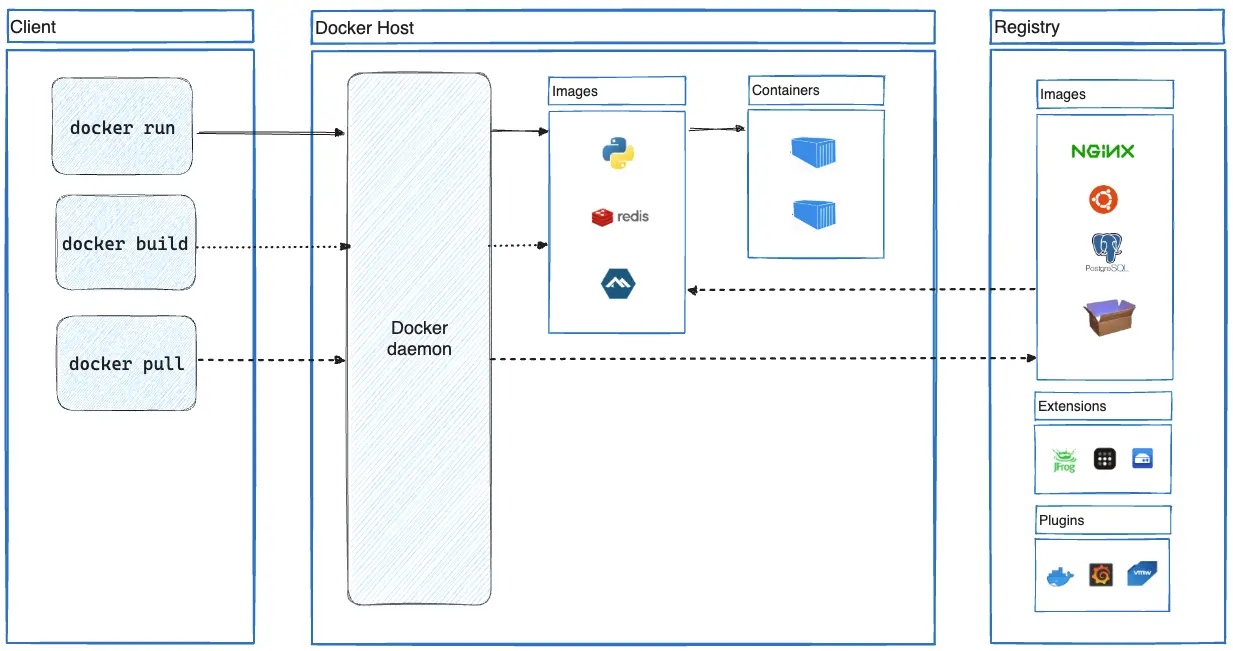
\includegraphics[width=0.8\textwidth]{media/docker_architecture.png}
  \legend{Fonte: Adaptado da documentação oficial do Docker \cite{docker_overview}.}
  \label{fig:docker-arquitetura}
\end{figure}

\subsection{Registries e distribuição de imagens}
\label{subsec:docker-registries}

Imagens são armazenadas em \textbf{registries} (Docker Hub público ou registries privados). Comandos como \texttt{docker pull}, \texttt{docker push} e \texttt{docker run} interagem com o registry configurado. Essa camada viabiliza portabilidade entre ambientes locais, datacenters e nuvens \cite{docker_overview}. 

\section{Objetos do Docker: imagens, camadas e contêineres}
\label{sec:docker-objetos}

\subsection{Imagens em camadas}
\label{subsec:docker-imagens}

Uma \textbf{imagem} é um \textit{template} somente leitura, composto por \textbf{camadas} (\textit{layers}). Cada instrução no \textbf{Dockerfile} cria uma nova camada. Em uma reconstrução, apenas camadas alteradas são recompostas, o que torna as imagens mais leves e o \textit{build} mais eficiente \cite{docker_overview}. 

\subsection{Contêineres}
\label{subsec:docker-containers}

Um \textbf{contêiner} é uma instância executável de uma imagem. Ele pode ser criado, iniciado, parado, removido e conectado a redes e volumes. Por padrão, um contêiner é isolado, mas o nível de isolamento de rede, armazenamento e \textit{namespaces} pode ser configurado. Alterações não persistentes são descartadas quando o contêiner é removido \cite{docker_overview}. 

\begin{codigo}[H]
\begin{lstlisting}[language=bash]
# Exemplo simples: criar um container Ubuntu e entrar em /bin/bash
docker run -it ubuntu /bin/bash
\end{lstlisting}
\caption{Exemplo de execução interativa de contêiner}
\label{lst:docker-run}
\end{codigo}

\section{Dockerfile: referência e instruções principais}
\label{sec:dockerfile}

O \textbf{Dockerfile} é um arquivo de texto que descreve, passo a passo, como montar uma imagem: cada instrução corresponde a um comando executado durante o \textit{build}. Entre as instruções mais comuns estão: \texttt{FROM}, \texttt{RUN}, \texttt{COPY}, \texttt{ADD}, \texttt{CMD}, \texttt{ENTRYPOINT}, \texttt{ENV}, \texttt{ARG}, \texttt{EXPOSE}, \texttt{WORKDIR}, \texttt{USER}, \texttt{VOLUME}, \texttt{HEALTHCHECK}, \texttt{LABEL} e \texttt{ONBUILD} \cite{dockerfile_ref}. 

\subsection{Formato, substituição de variáveis e \textit{.dockerignore}}
\label{subsec:dockerfile-format}

As instruções suportam formas \textit{shell} e \textit{exec} (JSON). Variáveis de ambiente podem ser interpoladas em várias instruções, respeitando o escopo e a ordem de avaliação. O arquivo \texttt{.dockerignore} exclui caminhos do contexto de \textit{build}, reduzindo tamanho de envio e prevenindo inclusão indevida de arquivos \cite{dockerfile_ref}. 

\subsection{Instruções essenciais}
\label{subsec:dockerfile-core}

\begin{itemize}
    \item \textbf{\texttt{FROM}}: define a imagem base e pode nomear estágios (\texttt{AS}). Suporta interação com \texttt{ARG} na seleção da base (por exemplo, plataforma/versão). \cite{dockerfile_ref} 
    
    \item \textbf{\texttt{RUN}}: executa comandos e compõe camadas; com BuildKit, permite \texttt{RUN --mount} para \textit{cache}, \textit{bind}, \textit{tmpfs}, \textit{secret} e \textit{ssh}, acelerando \textit{builds} e protegendo segredos. \cite{dockerfile_ref} 
    \item \textbf{\texttt{COPY}/\texttt{ADD}}: copiam arquivos do contexto; \texttt{COPY --from} permite copiar de outro estágio/imagem (\textit{multi-stage}). Flags como \texttt{--chown} e \texttt{--chmod} controlam propriedade e permissões. \cite{dockerfile_ref}
    \item \textbf{\texttt{CMD}/\texttt{ENTRYPOINT}}: definem o processo padrão; podem ser combinadas (por exemplo, \texttt{ENTRYPOINT} como executável e \texttt{CMD} como argumentos). \cite{dockerfile_ref}
    \item \textbf{\texttt{ENV}/\texttt{ARG}}: definem variáveis para \textit{build} e \textit{runtime} (sendo \texttt{ARG} não persistente na imagem final; cuidado para não vazar \textit{secrets} via \texttt{ENV}). \cite{dockerfile_ref}
    \item \textbf{\texttt{WORKDIR}/\texttt{USER}/\texttt{EXPOSE}/\texttt{VOLUME}}: definem diretório de trabalho, usuário não privilegiado, portas documentadas e pontos de montagem. \cite{dockerfile_ref}
    \item \textbf{\texttt{HEALTHCHECK}}: verifica saúde do contêiner; útil para orquestração e \acrshort{slo}s. \cite{dockerfile_ref}
\end{itemize}

\subsection{Boas Práticas de Construção}
\label{sec:docker-best-practices}

\subsection{Multi-stage builds e imagens enxutas}
\label{subsec:multi-stage}

\textbf{Multi-stage builds} permitem compilar artefatos em um estágio (com \textit{toolchains} pesadas) e copiar apenas o resultado para um estágio final mínimo (por exemplo, \texttt{alpine} ou \texttt{scratch}), reduzindo tamanho, superfície de ataque e tempo de transferência \cite{dockerfile_ref}.

\begin{codigo}[H]
\begin{lstlisting}[language=Dockerfile]
# syntax=docker/dockerfile:1
FROM node:20-alpine AS build
WORKDIR /app
COPY package*.json ./
RUN npm ci --omit=dev
COPY . .
RUN npm run build

FROM node:20-alpine AS runtime
WORKDIR /app
ENV NODE_ENV=production
# copia somente o que precisa para rodar
COPY --from=build /app/.next ./.next
COPY --from=build /app/package*.json ./
EXPOSE 3000
CMD ["node", ".next/standalone/server.js"]
\end{lstlisting}
\caption{Exemplo de multi-stage build para aplicação \acrshort{ssr} com Node/Next.js}
\label{lst:dockerfile-multistage}
\end{codigo}

\subsection{Cache de build e \texttt{RUN --mount}}
\label{subsec:cache-build}

Organize instruções do Dockerfile para maximizar \textbf{cache} (mudar menos camadas de cima). Com BuildKit, \texttt{RUN --mount=type=cache} cria caches persistentes para gerenciadores de pacotes (\texttt{apt}, \texttt{pip}, \texttt{go}) sem invalidar camadas, acelerando builds subsequentes \cite{dockerfile_ref}. 

\begin{codigo}[H]
\begin{lstlisting}[language=Dockerfile]
# syntax=docker/dockerfile:1
FROM ubuntu:24.04
RUN rm -f /etc/apt/apt.conf.d/docker-clean; \
    echo 'Binary::apt::APT::Keep-Downloaded-Packages "true";' \
    > /etc/apt/apt.conf.d/keep-cache
RUN --mount=type=cache,target=/var/cache/apt,sharing=locked \
    --mount=type=cache,target=/var/lib/apt,sharing=locked \
    apt-get update && apt-get install -y curl ca-certificates
\end{lstlisting}
\caption{Uso de cache de \texttt{apt} com BuildKit}
\label{lst:dockerfile-cache}
\end{codigo}

\subsection{\texttt{.dockerignore} e redução do contexto}
\label{subsec:dockerignore}

Use \texttt{.dockerignore} para excluir arquivos como \texttt{node\_modules}, \texttt{.git}, testes e artefatos locais. Isso reduz o contexto enviado ao daemon e evita vazamento de dados no \textit{build} \cite{dockerfile_ref}. 

\begin{codigo}[H]
\begin{lstlisting}[language=bash]
# .dockerignore (exemplo)
.git
node_modules
*.log
.env
tests/
docs/
\end{lstlisting}
\caption{Exemplo de \texttt{.dockerignore}}
\label{lst:dockerignore}
\end{codigo}

\subsection{Segredos e credenciais no build}
\label{subsec:secrets}

Evite inserir \textit{secrets} na imagem via \texttt{ENV}/\texttt{ARG}. Prefira \texttt{RUN --mount=type=secret} ou \texttt{--mount=type=ssh} para acesso temporário a chaves e tokens durante o \textit{build}. Esses valores não são gravados nas camadas finais \cite{dockerfile_ref}. 

\subsection{Rede, portas, volumes e saúde}
\label{sec:network-storage}

\textbf{Portas} podem ser documentadas com \texttt{EXPOSE}, enquanto o mapeamento real é definido em \texttt{docker run -p}. \textbf{Volumes} permitem persistência de dados; \textbf{redes} conectam múltiplos contêineres. \textbf{Healthchecks} ajudam a detectar falhas de \textit{runtime} e são úteis em composição e orquestração \cite{dockerfile_ref,docker_overview}.

\begin{codigo}[H]
\begin{lstlisting}[language=bash]
# Exemplo de execução com mapeamento de porta e volume
docker run -d --name web -p 8080:80 -v data:/var/lib/app myimage:1.0
\end{lstlisting}
\caption{Mapeamento de porta e volume em um contêiner}
\label{lst:docker-run-ports-vol}
\end{codigo}

\subsection{Fluxo de Trabalho: construir, \textit{taguear}, publicar e executar}
\label{sec:workflow}

O ciclo típico envolve: escrever o Dockerfile, \textbf{construir} (\texttt{docker build}), \textbf{taguear}, \textbf{publicar} a imagem (\texttt{docker push}) e \textbf{executar} (\texttt{docker run}). Com \textit{buildx}, pode-se produzir imagens multi-arquitetura e usar recursos avançados de cache \cite{docker_overview,dockerfile_ref}.

\begin{codigo}[H]
\begin{lstlisting}[language=bash]
# Build e tag
docker build -t ghcr.io/usuario/minhaapp:1.0 .

# Login e push no registry escolhido
docker login ghcr.io
docker push ghcr.io/usuario/minhaapp:1.0

# Execução mapeando porta
docker run -d -p 3000:3000 ghcr.io/usuario/minhaapp:1.0
\end{lstlisting}
\caption{Ciclo de construção, publicação e execução}
\label{lst:docker-workflow}
\end{codigo}

\subsection{Integração com o Estudo CSR x SSR}
\label{sec:docker-csr-ssr}

No contexto do seu trabalho, contêineres simplificam a comparação entre \acrshort{csr} e \acrshort{ssr} ao padronizar ambiente, dependências e execução:

\begin{itemize}
  \item \textbf{CSR/SSG (estático + CDN):} \textit{build} do frontend (React/Vite/Next SSG) em um estágio e \textbf{Nginx} no estágio final para servir arquivos estáticos.  
  \item \textbf{SSR (Node/Next):} multi-stage com instalação apenas das dependências de produção e \textbf{imagem enxuta} (\texttt{alpine} ou \texttt{distroless}), expondo a porta do servidor \acrshort{ssr}.
  \item \textbf{Medições reprodutíveis:} ao encapsular as variantes em imagens, é possível rodar os mesmos testes de desempenho (FCP, TTFB, INP, TTI) em hardware idêntico e com \textit{network shaping}, isolando o impacto da estratégia de renderização.
\end{itemize}

\begin{codigo}[H]
\begin{lstlisting}[language=Dockerfile]
# Nginx para app CSR/SSG (estático)
FROM nginx:1.27-alpine
COPY ./dist/ /usr/share/nginx/html
# (Opcional) Copiar nginx.conf customizado
# COPY ./nginx.conf /etc/nginx/conf.d/default.conf
EXPOSE 80
\end{lstlisting}
\caption{Servidor estático para aplicação CSR/SSG}
\label{lst:dockerfile-nginx-static}
\end{codigo}

\subsection{Síntese}
\label{sec:docker-sintese}

O Docker fornece uma base consistente para empacotar e executar aplicações, com \textbf{isolamento leve}, portabilidade e \textbf{ciclo de vida} claro (construir, distribuir, executar). O \textbf{Dockerfile} e as boas práticas descritas \textit{multi-stage}, cache de build, \texttt{.dockerignore} e \textit{secrets} viabilizam imagens menores, \textit{builds} mais rápidos e maior segurança. Tudo isso contribui diretamente para a reprodutibilidade e a comparabilidade dos experimentos entre \acrshort{csr} e \acrshort{ssr} \cite{docker_overview,dockerfile_ref}. 


\chapter{Trabalhos Relacionados}
\label{cap:trabalhos}
Este capítulo apresenta os trabalhos relacionados ao objeto de pesquisa obtidos utilizando o protocolo descrito na seção a seguir.

\section{Protocolo}
Esta seção apresenta o protocolo de mapeamento sistemático da literatura usado para atingir os objetivos da pesquisa.

\subsection{Questões de pesquisa}
\label{section:questoes_pesquisa}
\begin{enumerate}
    \item[Q1:] De que maneira a escolha entre \acrshort{csr} e \acrshort{ssr} influenciam a experiência do usuário?
    \item[Q2:] Como as abordagens \acrshort{csr} e \acrshort{ssr} afetam métricas de performance, tempo de carregamento e tempo até a interatividade em aplicações web?
    \item[Q3:] Quais são os principais desafios e \english{trade-offs} na implementação de \acrshort{csr} e \acrshort{ssr}?
\end{enumerate}

\subsection{Estratégia de busca}
Esta seção apresenta a estratégia de buscas de artigos científicos e livros relacionados à pesquisa. As ferramentas utilizadas para realizar as buscas são:
\begin{itemize}
    \item \textbf{Periódicos Capes:} É uma ferramenta disponibilizada pelo governo federal para uso de estudantes e pesquisadores. Acessando através da instituição de ensino ou pesquisa, é possível ter acesso completo a uma grande quantidade de artigos científicos publicados em variadas revistas, conferências e universidades. A principal vantagem dessa ferramenta é a possibilidade de ler o conteúdo integral de grande parte das publicações disponíveis. Por outro lado, as expressões de busca atualmente suportadas são bem limitadas.
    \item \textbf{\english{Scopus:}} Trata-se de um ferramenta similar ao Periódicos Capes. No entanto, o \english{Scopus} permite a elaboração de expressões de buscas mais complexas e sofisticadas, servindo para descobrir publicações não detectadas pelas outras plataformas. Além disso, possui um acervo bem mais amplo que o Periódicos Capes. Entretanto, algumas publicações não podem ser vistas na íntegra de forma gratuita.
    \item \textbf{\english{PICOC}}: A técnica \english{PICOC} foi utilizada para estruturar e refinar a estratégia de busca. Essa abordagem consiste em definir cinco elementos principais que auxiliam na formulação da expressão booleana para a pesquisa:
\begin{itemize}
    \item \textbf{P (População/Problema):} Define os estudos ou o grupo de interesse, ou seja, o problema ou a população que se deseja investigar. Por exemplo, “artigos que tratem da integração de tecnologias digitais na educação.”
    \item \textbf{I (Intervenção/Interesse):} Refere-se à intervenção, prática ou fenômeno que está sendo analisado. Neste caso, pode ser a “inserção de tecnologias digitais nos processos de ensino e aprendizagem.”
    \item \textbf{C (Comparação):} Descreve o(s) elemento(s) com os quais a intervenção ou situação é comparada, como “ensino tradicional” ou a comparação entre diferentes estratégias digitais, quando aplicável.
    \item \textbf{O (Outcome/Desfecho):} Indica os resultados ou efeitos esperados da intervenção. Por exemplo, “melhora do desempenho acadêmico” ou “maior engajamento dos alunos.”
    \item \textbf{C (Contexto):} Considera o ambiente ou cenário onde a intervenção ocorre, como “instituições de ensino, universidades” ou “publicações indexadas em bases internacionais.”
\end{itemize}
A partir da definição desses elementos, foi possível construir uma expressão booleana que unisse os principais termos de interesse para a pesquisa. Esse método colaborou para refinar os resultados, tornando a busca mais precisa e abrangente, conforme exemplificado no \autoref{quad:quadro_picoc}.
    \item \textbf{\english{Google Docs:}} Ferramenta desenvolvida pela \english{Google LLC} que permite a criação e edição de documentos de texto. Suas grandes vantagens em relação a ferramentas de outros fornecedores são as avançadas ferramentas de colaboração e a possibilidade de acesso por meio de navegadores \english{web}, sem necessidade de instalação de \english{software} específico.
    \item \textbf{\english{Google Sheets}}: Com as mesmas características e vantagens do \english{Google Docs}, essa ferramenta fornece recursos para elaboração de planilhas de cálculo. É muito útil para realizar análise de dados simples e também visualizar e apresentar dados tabulares.
\end{itemize}



% Como grande parte das publicações na área de computação são em inglês, esta pesquisa utiliza esse idioma para fazer buscas nas ferramentas indicadas. Além disso, \acrfull{csr} e \acrfull{ssr} são relativamente recentes, as buscas se limitaram a publicações feitas nos últimos 20 anos.

% Os termos-chave para realização das buscas são: Microsserviço, \acrshort{csr} e \acrlong{ssr}. Como a busca é feita em inglês, se usará \english{web performance} nas buscas.

\subsection{Quadro PICOC}
\label{section:quadro_picoc}

\begin{quadro}[H]
\centering

\setlength{\tabcolsep}{0.8em} % espaçamento horizontal
\renewcommand{\arraystretch}{1.5} % espaçamento vertical
\caption{Estrutura PICOC aplicada à pesquisa}
\begin{tabular}{|p{1.5in}|p{4.2in}|}
\hline
\textbf{Elemento} & \textbf{Descrição} \\ \hline

\textbf{P (População/Problema)} & 
Equipes de desenvolvimento web, arquitetos de software e gestores de TI que precisam escolher estratégias de renderização (\acrshort{csr} ou \acrshort{ssr}) para aplicações web modernas, visando otimizar desempenho, \acrshort{seo} e experiência do usuário. 
\\ \hline

\textbf{I (Intervenção)} & 
Adoção de técnicas de \textbf{\acrshort{csr}} (Client-Side Rendering): todo (ou quase todo) o conteúdo gerado no lado do cliente, utilizando frameworks/libraries como React, Vue, Angular etc.
\\ \hline

\textbf{C (Comparação)} & 
Implementação de \textbf{\acrshort{ssr}} (Server-Side Rendering): conteúdo pré-renderizado no servidor antes de ser enviado ao cliente, usando \emph{meta-frameworks} como Next.js, Nuxt.js, SvelteKit, Angular Universal, entre outros.
\\ \hline

\textbf{O (Outcome / Resultado)} & 
\begin{itemize}
  \item Métricas de desempenho (tempo de carregamento, \textit{time-to-first-byte}, \textit{largest contentful paint}, etc.)
  \item Impacto no \textbf{\acrshort{seo}} (indexabilidade, posicionamento em buscadores)
  \item Experiência do usuário e usabilidade
  \item Escalabilidade do sistema (uso de recursos de servidor/cliente)
\end{itemize}
\\ \hline

\textbf{C (Contexto)} & 
Aplicações web modernas que buscam equilibrar interatividade, rapidez de carregamento, otimização para motores de busca e redução de custos operacionais. O estudo pode ser aplicado a sistemas de e-commerce, portais de conteúdo, \emph{landing pages}, etc.
\\ \hline

\end{tabular}
\label{quad:quadro_picoc}
\fonte{os autores}
\end{quadro}


\subsection{Expressão de busca}
\label{section:string_busca}

\begin{quadro}[H]
\centering

\setlength{\tabcolsep}{0.8em} % for the horizontal padding
\renewcommand{\arraystretch}{1.5}% for the vertical padding
\caption{Expressão de busca utilizada}
\begin{tabular}{|p{4.5in}|}

\hline
Expressão de Busca \\ \hline
\english{(TITLE-ABS-KEY("Client-Side Rendering" OR "CSR" OR "Server-Side Rendering" OR "SSR")) AND (TITLE-ABS-KEY("web performance" OR "page speed" OR "web optimization" OR "SEO" OR "search engine optimization" OR "user experience" OR "UX" OR "usability"))} \\ \hline

\end{tabular}
\label{quad:string_busca}
\fonte{os autores}
\end{quadro}

\subsection{Estratégia de seleção}
\label{section:estrategia_selecao}
A estratégia de seleção dos artigos foi baseada em critérios de inclusão e exclusão, conforme descrito a seguir:
\begin{itemize}
    \item \textbf{Critérios de inclusão:}
    \begin{itemize}
        \item Artigos publicados entre 2015 e 2025.
        \item Artigos que abordem o impacto de \acrshort{csr} e \acrshort{ssr} em aplicações web.
        \item Artigos que apresentem resultados de experimentos ou estudos de caso relacionados a \acrshort{csr} e \acrshort{ssr}.
    \end{itemize}
    \item \textbf{Critérios de exclusão:}
    \begin{itemize}
        \item Artigos que não estejam disponíveis na íntegra.
        \item Artigos que não abordem diretamente o tema da pesquisa.
        \item Artigos que sejam duplicados ou muito semelhantes a outros já selecionados.
    \end{itemize}
\end{itemize}

\section{Caracterização de pesquisa}
\label{section:caracterizacao_pesquisa}
Na \autoref{fig:docs_by_year}, é apresentado o número de publicações identificadas por ano, no intervalo entre 2020 e 2025. Observa-se um crescimento progressivo de 2020 a 2023, culminando em um pico em 2023, com 15 documentos publicados. A partir desse ponto, nota-se uma queda significativa: em 2024, o número de publicações cai para 9, e em 2025 esse número se reduz ainda mais, atingindo apenas 3 documentos. Essa redução pode ser parcialmente atribuída ao fato de que a coleta foi realizada no mês de abril de 2025, o que possivelmente não contempla todas as publicações previstas para o ano. No total, foram encontrados 50 documentos relevantes, distribuídos de forma desigual, evidenciando uma tendência crescente de interesse pelo tema até 2023, seguido de uma possível estabilização ou atraso na indexação dos dados mais recentes.

\begin{figure}[H]
    \centering
    \caption{Número de publicações ao longo dos anos}
    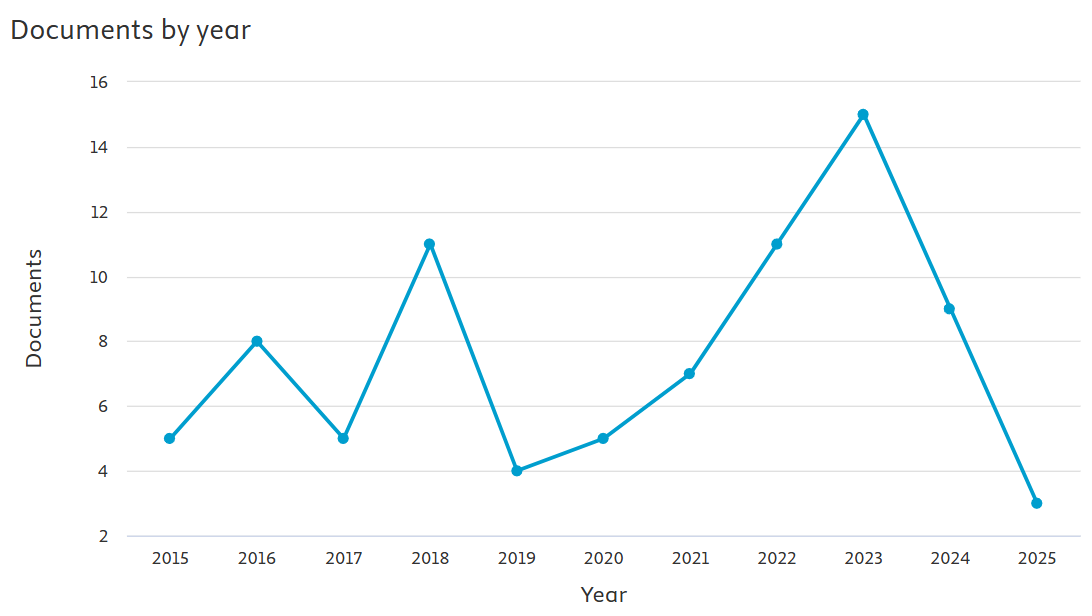
\includegraphics[width=0.9\textwidth]{media/docs_by_year.png}
    \legend{Fonte: Scopus}
    \label{fig:docs_by_year}
\end{figure}

Na \autoref{fig:docs_by_country} são apresentados os países com maior número de publicações relacionadas ao tema desta pesquisa. Observa-se que a China lidera com 10 documentos, seguida pela Alemanha (7) e pelos Estados Unidos (6). Em seguida, aparecem Índia, Reino Unido e Suíça, cada um com 5 documentos publicados. A Turquia também se destaca com 4 publicações, enquanto Croácia, Estônia e França completam a lista com 2 documentos cada. Esses dados evidenciam uma concentração relevante de estudos em países com infraestrutura tecnológica consolidada, especialmente na Ásia, Europa Ocidental e América do Norte, o que reforça o caráter global do interesse em torno da comparação entre abordagens de renderização no desenvolvimento de aplicações web.

\begin{figure}[H]
    \centering
    \caption{Distribuição das publicações por país}
    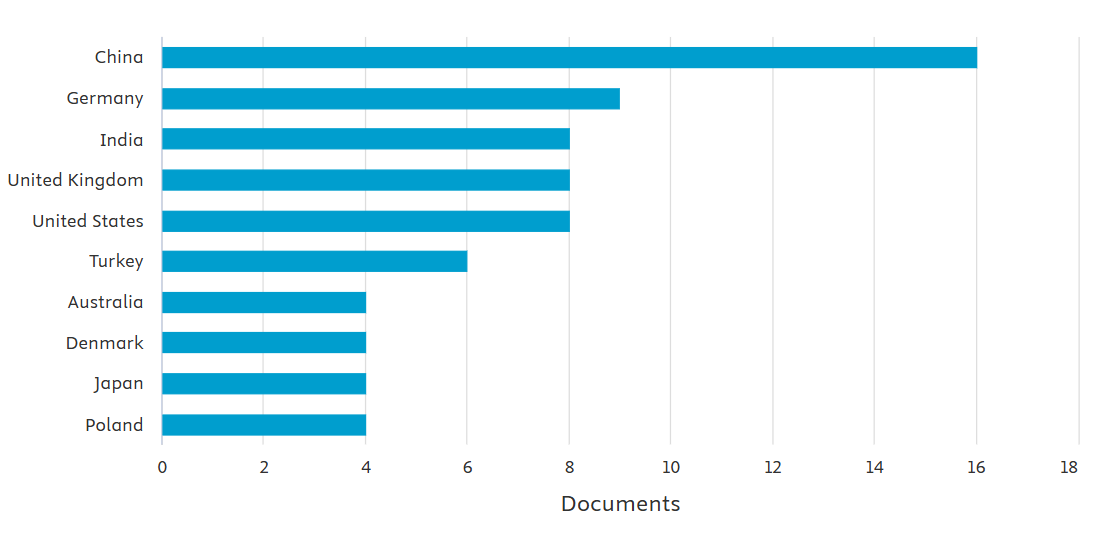
\includegraphics[width=0.9\textwidth]{media/docs_by_country.png}
    \legend{Fonte: Scopus}
    \label{fig:docs_by_country}
\end{figure}


\section{Artigos selecionados}
\label{section:artigos_selecionados}



\section{Resultados e Discussão}
\label{section:resultados_discussao}


% https://www-scopus-com.ez135.periodicos.capes.gov.br/results/results.uri?sort=plf-f&src=s&sid=c5e620a132b74a852dccc08c5c330e9d&sot=a&sdt=cl&sl=247&s=%28TITLE-ABS-KEY%28%22Client-Side+Rendering%22+OR+%22CSR%22+OR+%22Server-Side+Rendering%22+OR+%22SSR%22%29%29+AND+%28TITLE-ABS-KEY%28%22web+performance%22+OR+%22page+speed%22+OR+%22web+optimization%22+OR+%22SEO%22+OR+%22search+engine+optimization%22+OR+%22user+experience%22+OR+%22UX%22+OR+%22usability%22%29%29&origin=resultslist&editSaveSearch=&txGid=584773b92f904689225d6d8bd0143429&sessionSearchId=c5e620a132b74a852dccc08c5c330e9d&limit=10&yearFrom=2020&yearTo=2025


\chapter{Metodologia}
\label{cap:metodologia}

Este capítulo detalha a abordagem metodológica adotada para a condução do trabalho. A metodologia foi estruturada em quatro etapas principais: o levantamento teórico para fundamentar a pesquisa, o mapeamento sistemático da literatura para identificar o estado da arte, o desenvolvimento de um estudo de caso prático para a coleta de dados empíricos e, por fim, os procedimentos de teste e análise utilizados para comparar as arquiteturas \acrshort{csr} e \acrshort{ssr}.


\section{Levantamento Teórico}
\label{sec:levantamento-teorico}

O levantamento teórico consistiu na revisão e sistematização dos principais conceitos, tecnologias e práticas relacionadas à renderização de conteúdo em aplicações web, com foco nas abordagens de \english{\acrfull{csr}} e \english{\acrfull{ssr}}. Essa etapa teve como objetivo fornecer o embasamento necessário para o desenvolvimento do estudo de caso e da análise comparativa proposta neste trabalho.

A fundamentação iniciou-se com a exploração dos princípios do desenvolvimento web moderno, incluindo a arquitetura cliente-servidor, o funcionamento do protocolo \acrshort{http} e as tecnologias essenciais do \textit{frontend}: \acrshort{html}, \acrshort{css} e JavasSript. Estes elementos formam a base para compreender como as estratégias de renderização operam, tanto no lado do cliente quanto no lado do servidor.

Em seguida, foram estudadas em detalhes as abordagens \acrshort{csr} e \acrshort{ssr}. A renderização no lado do cliente (\acrshort{csr}) foi analisada quanto ao seu funcionamento típico em aplicações \english{\acrfull{spa}}, caracterizadas por uma única página carregada inicialmente, com atualizações dinâmicas de conteúdo via JavaScript. Essa abordagem oferece vantagens como maior interatividade e fluidez na navegação, além de transições rápidas entre páginas internas. No entanto, apresenta desvantagens como maior tempo de carregamento inicial e limitações de indexação por mecanismos de busca.

Por outro lado, a renderização no lado do servidor (\acrshort{ssr}) foi abordada sob a ótica de desempenho inicial otimizado e maior compatibilidade com \acrshort{seo}, pois o conteúdo é entregue já renderizado ao navegador. Essa abordagem é comumente utilizada em aplicações do tipo \english{\acrfull{mpa}}, que possuem múltiplas páginas distintas e se beneficiam da pré-renderização para melhorar a performance inicial, a acessibilidade e a visibilidade em mecanismos de busca. Como contraponto, o SSR demanda maior processamento no servidor e pode aumentar a complexidade da infraestrutura.

O levantamento teórico foi aprofundado com uma análise dos principais \textit{frameworks} e bibliotecas que materializam as arquiteturas \acrshort{csr} e \acrshort{ssr}. Foi dada ênfase especial ao \textit{React}, como principal expoente da renderização no lado do cliente, e ao \textit{Next.js}, \textit{framework} que o estende para possibilitar uma renderização robusta no lado do servidor. A discussão foi enriquecida com o estudo do ecossistema de outras ferramentas, como \textit{Vue.js} e \textit{Angular}, para consolidar a compreensão sobre os impactos de cada abordagem na experiência do usuário (\acrshort{ux}), no \acrshort{seo}, na acessibilidade e na interatividade.

Essa base teórica consolidada foi, portanto, essencial para embasar as escolhas metodológicas, delimitar o escopo do mapeamento da literatura e, principalmente, para orientar o desenvolvimento e a avaliação do estudo de caso prático detalhado a seguir.

\section{Mapeamento Sistemático da Literatura}
\label{sec:mapemento-sistematico-da-literatura}

O mapeamento sistemático da literatura teve como objetivo identificar, selecionar e analisar estudos acadêmicos relevantes que abordassem comparações entre as abordagens de renderização \english{\acrshort{csr}} e \english{\acrshort{ssr}} no contexto do desenvolvimento de aplicações web. Essa etapa foi essencial para compreender o estado da arte, bem como identificar lacunas e oportunidades para a realização do estudo de caso proposto neste trabalho.

A estratégia de busca foi estruturada com o apoio da metodologia \textit{PICOC}, que define os elementos População, Intervenção, Comparação, Resultado e Contexto, com o intuito de guiar a construção das expressões de busca e garantir abrangência e precisão nos resultados. As principais bases de dados utilizadas incluíram Periódicos Capes e Scopus, por oferecerem amplo acervo e suporte a pesquisas refinadas.

Foram utilizadas expressões booleanas combinando termos como \textit{Client-Side Rendering}, \textit{Server-Side Rendering}, \textit{Web Performance}, \textit{SEO}, \textit{UX} e \textit{Frontend Architecture}. Após a aplicação dos critérios de inclusão e exclusão, os artigos resultantes foram classificados e analisados de acordo com sua relevância, tipo de abordagem estudada, metodologias utilizadas e principais conclusões.

A seleção final contemplou trabalhos que abordavam métricas de desempenho, tempo de carregamento, interatividade, \acrshort{seo} e experiência do usuário. Além disso, foram considerados estudos que analisavam o uso de frameworks modernos como \textit{React}, \textit{Next.js}, \textit{Nuxt.js} e \textit{Angular Universal}, além de pesquisas aplicadas em contextos reais de produção.

Como resultado, foi possível consolidar uma visão abrangente sobre os desafios, vantagens e limitações de cada abordagem, fornecendo subsídios importantes para a execução do estudo de caso prático apresentado nos capítulos seguintes. O mapeamento sistemático também evidenciou a escassez de estudos nacionais aplicados ao tema, reforçando a relevância deste trabalho no cenário acadêmico e profissional brasileiro.


\section{Estudo de Caso Prático}
\label{sec:estudo-de-caso-pratico}

Para materializar a análise comparativa proposta, esta pesquisa se baseia em um estudo de caso prático: o desenvolvimento de uma aplicação web de notícias sobre tecnologia. Este contexto foi escolhido por ser altamente representativo de um vasto segmento de aplicações focadas em conteúdo, onde a velocidade de carregamento inicial e a otimização para mecanismos de busca (\acrshort{seo}) são fatores críticos para a retenção de usuários e o sucesso do produto.

Com o objetivo de estabelecer condições equivalentes para comparação, foram desenvolvidas duas versões funcionalmente idênticas da plataforma. A primeira utiliza \acrfull{csr}, implementada com a biblioteca \textit{React} (\acrshort{spa}), enquanto a segunda adota \acrfull{ssr}, com o \textit{framework Next.js} (\acrshort{mpa}). Ambas as versões consomem dados da mesma \textit{API} externa de notícias e apresentam a mesma interface e funcionalidades como listagem de artigos, busca e visualização de detalhes, assegurando que as diferenças de desempenho observadas possam ser diretamente atribuídas à arquitetura de renderização empregada.

Cada versão foi implementada seguindo os princípios fundamentais da sua respectiva abordagem. Na aplicação \acrshort{csr}, a renderização ocorre predominantemente no navegador do usuário, ao passo que na versão \acrshort{ssr}, o conteúdo HTML é pré-renderizado no servidor e enviado pronto ao cliente. Ambas as implementações foram submetidas a um protocolo de testes para a coleta de dados, conforme detalhado na seção seguinte, permitindo uma análise equitativa e baseada em evidências.


\section{Coleta de Dados e Testes}
\label{sec:coleta-de-dados-e-testes}

Esta seção descreve o procedimento de coleta e análise dos dados obtidos a partir da comparação entre as aplicações desenvolvidas com \english{\acrshort{csr}} e \english{\acrshort{ssr}}. O objetivo é mensurar o desempenho, a eficiência e a experiência do usuário proporcionada por cada aplicação sob condições controladas.

\subsection{Definição das Métricas}

A medição de desempenho em aplicações web modernas evoluiu de uma simples análise do tempo de carregamento total para uma avaliação multifacetada da experiência do usuário (UX). Para padronizar essa medição, o Google introduziu a iniciativa Web Vitals, um conjunto de métricas que quantificam aspectos cruciais da jornada do usuário. O subconjunto mais importante, conhecido como Core Web Vitals, foca em três pilares da experiência: o carregamento (medido pelo \acrshort{lcp}), a interatividade (medida pelo \acrshort{inp}) e a estabilidade visual (medida pelo \acrshort{cls}).

Adotando essa metodologia como padrão de mercado, este trabalho selecionou um conjunto de indicadores para realizar uma avaliação completa, abrangendo não apenas a percepção do usuário, mas também os custos computacionais no servidor. Para garantir uma análise estruturada, as métricas foram categorizadas da seguinte forma:

\begin{itemize}
\item Web Vitals (Núcleo): Representam a base da análise de experiência do usuário. Foram coletadas as métricas \acrfull{ttfb}, \acrfull{fcp}, \acrfull{lcp}, \acrfull{cls} e \acrfull{inp}. Esses dados foram registrados diretamente no cliente durante a navegação real e persistidos em formato NDJSON para análise posterior.

\item Auditoria de Laboratório (Apoio): Utilizando o Lighthouse, foram realizadas auditorias complementares para analisar o \acrfull{tbt} e identificar oportunidades de otimização. As auditorias também validaram aspectos de Acessibilidade e \acrshort{seo} de forma automatizada.

\item Recursos do Servidor (Custo): Para contextualizar o custo de execução de cada abordagem, o consumo de recursos dos contêineres foi monitorado com o comando \texttt{docker stats}, registrando o uso de CPU e memória durante os testes.
\end{itemize}



Adicionalmente, foram observados: número de requisições HTTP e uso de cache (no cliente), bem como consumo de recursos do contêiner (CPU e memória) durante os testes. O \acrfull{tti} foi empregado apenas como métrica de \textit{laboratório} via Lighthouse, não integrando o conjunto atual de Core Web Vitals. O tratamento estatístico detalhado das métricas será apresentado posteriormente.

\subsection{Ferramentas de Teste}

Foram utilizadas ferramentas complementares, com ênfase na coleta contínua no navegador (\textit{field}) e apoio de auditoria em \textit{laboratório}:

\begin{itemize}
    \item Web Vitals (\acrfull{rum}): Instrumentação no cliente para coletar as métricas TTFB, FCP, LCP, CLS e INP. O envio dos dados a um endpoint interno é feito via \texttt{navigator.sendBeacon}, uma API que garante a transmissão confiável das métricas mesmo quando o usuário encerra a página, com os dados persistidos em formato NDJSON;

    \item Google Lighthouse (auxiliar): Auditoria em \textit{laboratório} para Performance (incluindo FCP, LCP, CLS, Speed Index e TBT), executada localmente sobre os serviços em Docker;
    \item Chrome DevTools: Inspeção de rede, \textit{waterfall}, cache e verificação dos \textit{POSTs} de métricas;
    \item docker stats: Acompanhamento do uso de CPU e memória dos contêineres durante a execução dos testes.
\end{itemize}

\subsection{Ambiente de Testes}


Os testes para ambas as versões (\acrshort{csr} e \acrshort{ssr}) foram conduzidos em um ambiente local, utilizando contêineres \textit{Docker} para garantir a consistência. A escolha por essa abordagem foi uma consequência direta das restrições do plano de desenvolvedor (gratuito) da NewsAPI. Especificamente, a política de uso deste plano restringe as chamadas da API a requisições que partem de localhost, o que inviabilizou um teste em produção. No caso da versão \acrshort{csr}, a política de CORS bloquearia as chamadas diretas do navegador em um domínio público; já para a versão \acrshort{ssr}, as chamadas de servidor para servidor seriam igualmente bloqueadas, pois o servidor de produção não seria localhost. Portanto, a execução local não apenas contornou essa limitação, mas também assegurou um maior controle sobre as variáveis do experimento e a total reprodutibilidade dos resultados. Ambos os serviços foram executados com paridade de recursos:

\begin{itemize}
    \item CPU: \texttt{--cpus="1.0"} e \texttt{--cpuset-cpus="0"};
    \item Memória: \texttt{--memory="1g"} e \texttt{--memory-swap="1g"};
    \item Sistema de arquivos: \texttt{--read-only} com \texttt{--tmpfs /tmp};
    \item Persistência de métricas: volume em \texttt{/data} com \texttt{METRICS\_PATH=/data/webvitals.ndjson}.
\end{itemize}

A aplicação \acrshort{ssr} (Next.js) foi empacotada em modo \textit{standalone}. A aplicação \acrshort{csr} (React + Vite) foi servida por um processo \texttt{Node.js} simples que também expõe o endpoint de métricas. Os serviços públicos locais utilizados nos testes foram:
\begin{itemize}
    \item SSR/Next.js: \texttt{http://localhost:3001}
    \item CSR/React: \texttt{http://localhost:3002}
\end{itemize}

\subsection{Execução dos Testes}

A execução foi conduzida em quatro etapas, sendo:

\begin{enumerate}
    \item Aquecimento: duas visitas iniciais à mesma rota em cada aplicação, para estabilização de caches e recursos;
    \item Coleta principal (Web Vitals): navegação real em janela anônima, registrando TTFB, FCP, LCP, CLS e INP por meio do endpoint interno e persistindo em arquivo NDJSON;
    \item Coleta auxiliar (Lighthouse): auditorias repetidas em modo desktop, com parâmetros de \textit{throttling} consistentes entre cenários, para fornecer referência de \textit{laboratório};
    \item Observabilidade do contêiner: monitoramento pontual com \texttt{docker stats} para CPU e memória durante as execuções.
\end{enumerate}


Para reduzir a variabilidade, cada teste foi repetido no mínimo cinco vezes por cenário. A análise detalhada dos dados coletados, incluindo a quantidade total de repetições e o método de agregação estatística (mediana/p50 e p95), é apresentada no \textbf{Capítulo de Resultados e Discussão (\autoref{cap:resultados})}.

\subsection{Tratamento e Análise dos Dados}

Os dados coletados pela instrumentação (\acrshort{rum}) foram armazenados em arquivos NDJSON separados por abordagem, contendo os campos de identificação da métrica, valor e carimbo temporal. As auditorias do Lighthouse foram salvas em arquivos JSON/HTML para futura referência. Em seguida, os dados foram consolidados em planilhas, organizados por data, métrica e abordagem (CSR/SSR), preparando o conjunto de dados para a análise comparativa.

A análise foi conduzida por meio de estatísticas descritivas, com foco nas medianas p50 e p95, além de médias e desvios padrão quando apropriado. As comparações entre \acrshort{csr} e \acrshort{ssr} foram realizadas métrica a métrica (TTFB, FCP, LCP, CLS e INP), considerando os \textit{trade-offs} de cada abordagem. Os gráficos e tabelas de síntese resultantes dessa análise são apresentados no capítulo de Resultados e Discussões.

% \chapter{Cronograma}
\label{cap:cronograma}

% Defina as cores utilizadas
\definecolor{softCyan1}{HTML}{B2EBF2}     
\definecolor{softCyan2}{HTML}{4DD0E1}      
\definecolor{vividTurquoise}{HTML}{00E5FF} 
\definecolor{emeraldSea}{HTML}{26C6DA}     
\definecolor{deepTeal}{HTML}{00838F}       
\definecolor{darkEmerald}{HTML}{7FFFD4}    

\begin{quadro}[H]
    \centering
    \caption{Cronograma de execução da primeira etapa do TCC}
    \label{tab:cronograma_etapa1}
    \renewcommand{\arraystretch}{1.5}
    \begin{tabular}{|>{\centering\arraybackslash}p{3.5cm}|>{\centering\arraybackslash}p{1.25cm}|>{\centering\arraybackslash}p{1.25cm}|>{\centering\arraybackslash}p{1.25cm}|>{\centering\arraybackslash}p{1.25cm}|>{\centering\arraybackslash}p{1.25cm}|>{\centering\arraybackslash}p{1.25cm}|>{\centering\arraybackslash}p{1.25cm}|}
    \hline
    \textbf{Atividades} & \textbf{Nov} & \textbf{Dez} & \textbf{Jan} & \textbf{Fev} & \textbf{Mar} & \textbf{Abr} & \textbf{Mai} \\
    \hline
    Definição de tema e análise de artigos relevantes & \cellcolor{softCyan1} & \cellcolor{softCyan1} &  &  &  &  & \\
    \hline
    Apresentação da proposta de projeto e desenvolvimento da introdução &  &  & \cellcolor{softCyan2} & \cellcolor{softCyan2}  &  &  & \\
    \hline
    Definição do problema de pesquisa e Justificativa &  &  &  &   \cellcolor{vividTurquoise} & \cellcolor{vividTurquoise} &   & \\
    \hline
    Fundamentação teórica e trabalhos relacionados &  &  &  &  & \cellcolor{emeraldSea} & \cellcolor{emeraldSea} & \\
    \hline
    Revisão de literatura sobre renderização desempenho web em abordagens CSR e SSR &  &  &  &  & \cellcolor{deepTeal} & \cellcolor{deepTeal} & \cellcolor{deepTeal} \\
    \hline
    Apresentação do relatório final de TCC 1, com metodologia detalhada e cronograma atualizado &  &  &  &  &  & \cellcolor{darkEmerald} & \cellcolor{darkEmerald} \\
    \hline
    \end{tabular}
    \fonte{os autores}
\end{quadro}

\begin{quadro}[H]
    \centering
    \caption{Cronograma de execução da segunda etapa do TCC}
    \label{tab:cronograma_etapa2}
    \renewcommand{\arraystretch}{1.5}
    \begin{tabular}{|>{\centering\arraybackslash}p{3.5cm}|>{\centering\arraybackslash}p{1.25cm}|>{\centering\arraybackslash}p{1.25cm}|>{\centering\arraybackslash}p{1.25cm}|>{\centering\arraybackslash}p{1.25cm}|>{\centering\arraybackslash}p{1.25cm}|>{\centering\arraybackslash}p{1.25cm}|>{\centering\arraybackslash}p{1.25cm}|}
    \hline
    \textbf{Atividades} & \textbf{Jun} & \textbf{Jul} & \textbf{Ago} & \textbf{Set} & \textbf{Out} & \textbf{Nov} \\
    \hline
    Planejamento e definição do escopo da aplicação prática & \cellcolor{softCyan1} &  &  &  &  & \\
    \hline
    Desenvolvimento das aplicações com CSR e SSR &  & \cellcolor{softCyan2} & \cellcolor{softCyan2} & \cellcolor{softCyan2} &  & \\
    \hline
    Execução de testes de desempenho &  &  &  & \cellcolor{emeraldSea} & \cellcolor{emeraldSea} & \\
    \hline
    Avaliação e comparação dos resultados obtidos &  &  &  &  & \cellcolor{deepTeal} &  \\
    \hline
    Consolidação da conclusão do estudo &  &  &  &  & \cellcolor{darkEmerald} & \cellcolor{darkEmerald} \\
    \hline
    Revisão e entrega do relatório final do TCC 2 &  &  &  &  &  & \cellcolor{vividTurquoise} \\
    \hline
    \end{tabular}
    \fonte{os autores}
\end{quadro}



\chapter{Estudo de Caso: Desenvolvimento da Plataforma WallTech}
\label{cap:estudo_caso_dev}

Este capítulo detalha a construção do estudo de caso prático, que se baseia no cenário de uma empresa fictícia e no desenvolvimento de sua plataforma de notícias sobre tecnologia, a "WallTech". Serão apresentados o contexto do projeto, os requisitos funcionais, a organização do processo de desenvolvimento, os métodos de design, a implementação das arquiteturas \acrshort{csr} e \acrshort{ssr}, e os testes comparativos realizados.
\section{Contexto}
\label{section:contexto}

Este estudo de caso parte do cenário de uma empresa fictícia do setor de notícias sobre tecnologia, cujo objetivo é fornecer conteúdos atualizados e relevantes sobre inovações e tendências do mercado. O público-alvo inclui entusiastas de tecnologia, profissionais da área e usuários que desejam acompanhar as novidades do setor em diferentes dispositivos, graças a uma interface responsiva.

A Figura \ref{fig:wireframe-walltech} apresenta o \textit{wireframe} da plataforma \textbf{WallTech}, gerado com o auxílio da ferramenta \textbf{V0.dev}, que utiliza inteligência artificial para criar protótipos de interfaces a partir de descrições textuais. Esse modelo visual orienta a organização dos elementos na interface antes da implementação das versões em \acrshort{csr} e \acrshort{ssr}.

\begin{figure}[H]
  \centering
  \caption{Wireframe da plataforma WallTech}
  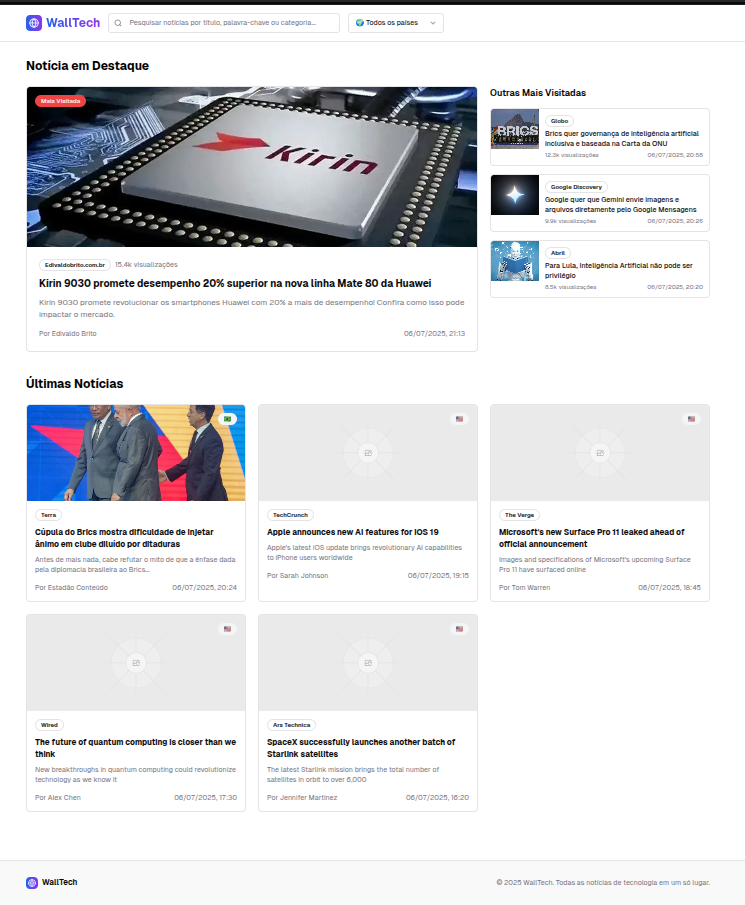
\includegraphics[width=0.7\textwidth]{media/wall_tech_wireframe.png}
  \legend{Fonte: os autores.}
  \label{fig:wireframe-walltech}
\end{figure}

Para analisar o impacto de diferentes abordagens de renderização web, foram desenvolvidos dois protótipos independentes da plataforma \textbf{WallTech}. O primeiro segue a abordagem de \acrfull{csr}, estruturado como uma \acrfull{spa} utilizando a biblioteca \textit{React}. O segundo utiliza \acrfull{ssr}, implementado como uma \acrfull{mpa} com o framework \textit{Next.js}.

A Figura \ref{fig:caso-uso-walltech} apresenta o diagrama de caso de uso da plataforma, destacando as principais funcionalidades acessíveis a usuários anônimos, como visualizar notícias recentes, acessar detalhes e realizar buscas por palavras-chave.

\begin{figure}[H]
  \centering
  \caption{Diagrama de caso de uso da plataforma WallTech}
  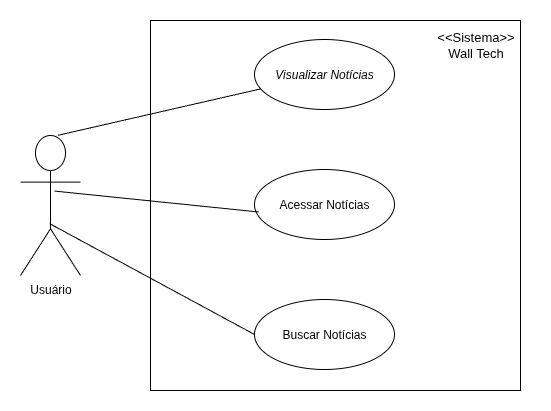
\includegraphics[width=0.7\textwidth]{media/wall_tech_use_case.png}
  \legend{Fonte: os autores.}
  \label{fig:caso-uso-walltech}
\end{figure}


\section{Processo de Desenvolvimento}
\label{section:processo-desenvolvimento}
O processo de desenvolvimento utilizado para construir a plataforma WallTech segue a metodologia ágil \english{Kanban}. Essa metodologia de desenvolvimento ágil é baseada em um quadro de tarefas, no qual cada tarefa é representada por um cartão \cite{gomes2014kanban}. O quadro Kanban é dividido em colunas que representam o estado atual de cada tarefa. As colunas mais comuns são: \english{To Do}, \english{In Progress} e \english{Done}, e o quadro é atualizado conforme as tarefas são realizadas. Além dessas colunas, o processo foi adaptado para incluir colunas adicionais como \english{Docs} e \english{Test}, permitindo que a documentação e os testes fossem gerenciados de forma organizada e eficiente durante o desenvolvimento.

A Figura \ref{fig:kanban-walltech} apresenta um exemplo do quadro Kanban utilizado no \english{GitHub Projects}, mostrando a organização das tarefas e o progresso do desenvolvimento da plataforma WallTech. O quadro reflete a estrutura de colunas adaptada, proporcionando uma visão clara do fluxo de trabalho da equipe, o que facilita o acompanhamento das tarefas em diferentes estágios.

Após a definição das funcionalidades principais do sistema, as tarefas foram inicialmente documentadas como \english{user stories}. As \english{user stories} são descrições simples e compreensíveis das funcionalidades a serem implementadas, permitindo uma comunicação clara entre a equipe de desenvolvimento e as partes interessadas. Cada \english{user story} é associada a um conjunto de requisitos específicos e uma definição de pronto, facilitando a compreensão do que precisa ser desenvolvido.

A partir dessas \english{user stories}, as \english{issues} foram criadas no \english{GitHub Projects}. Cada \english{issue} representa uma tarefa específica que deve ser realizada, baseada nas \english{user stories}. No \english{GitHub Projects}, essas \english{issues} são organizadas nas colunas do quadro Kanban, permitindo que a equipe visualize o progresso de cada tarefa e as mova conforme o andamento do trabalho.

A Figura \ref{fig:kanban-userstories} mostra um exemplo de cartão \english{issue} no \english{GitHub Projects}, ilustrando como as \english{user stories} são transformadas em tarefas e organizadas dentro do quadro Kanban. Cada \english{issue} possui detalhes sobre a tarefa, como descrições, prioridade e prazo, facilitando o gerenciamento e a execução das atividades no time de desenvolvimento.

\begin{figure}[H]
  \centering
  \caption{Exemplo de quadro Kanban no \english{GitHub Projects}}
  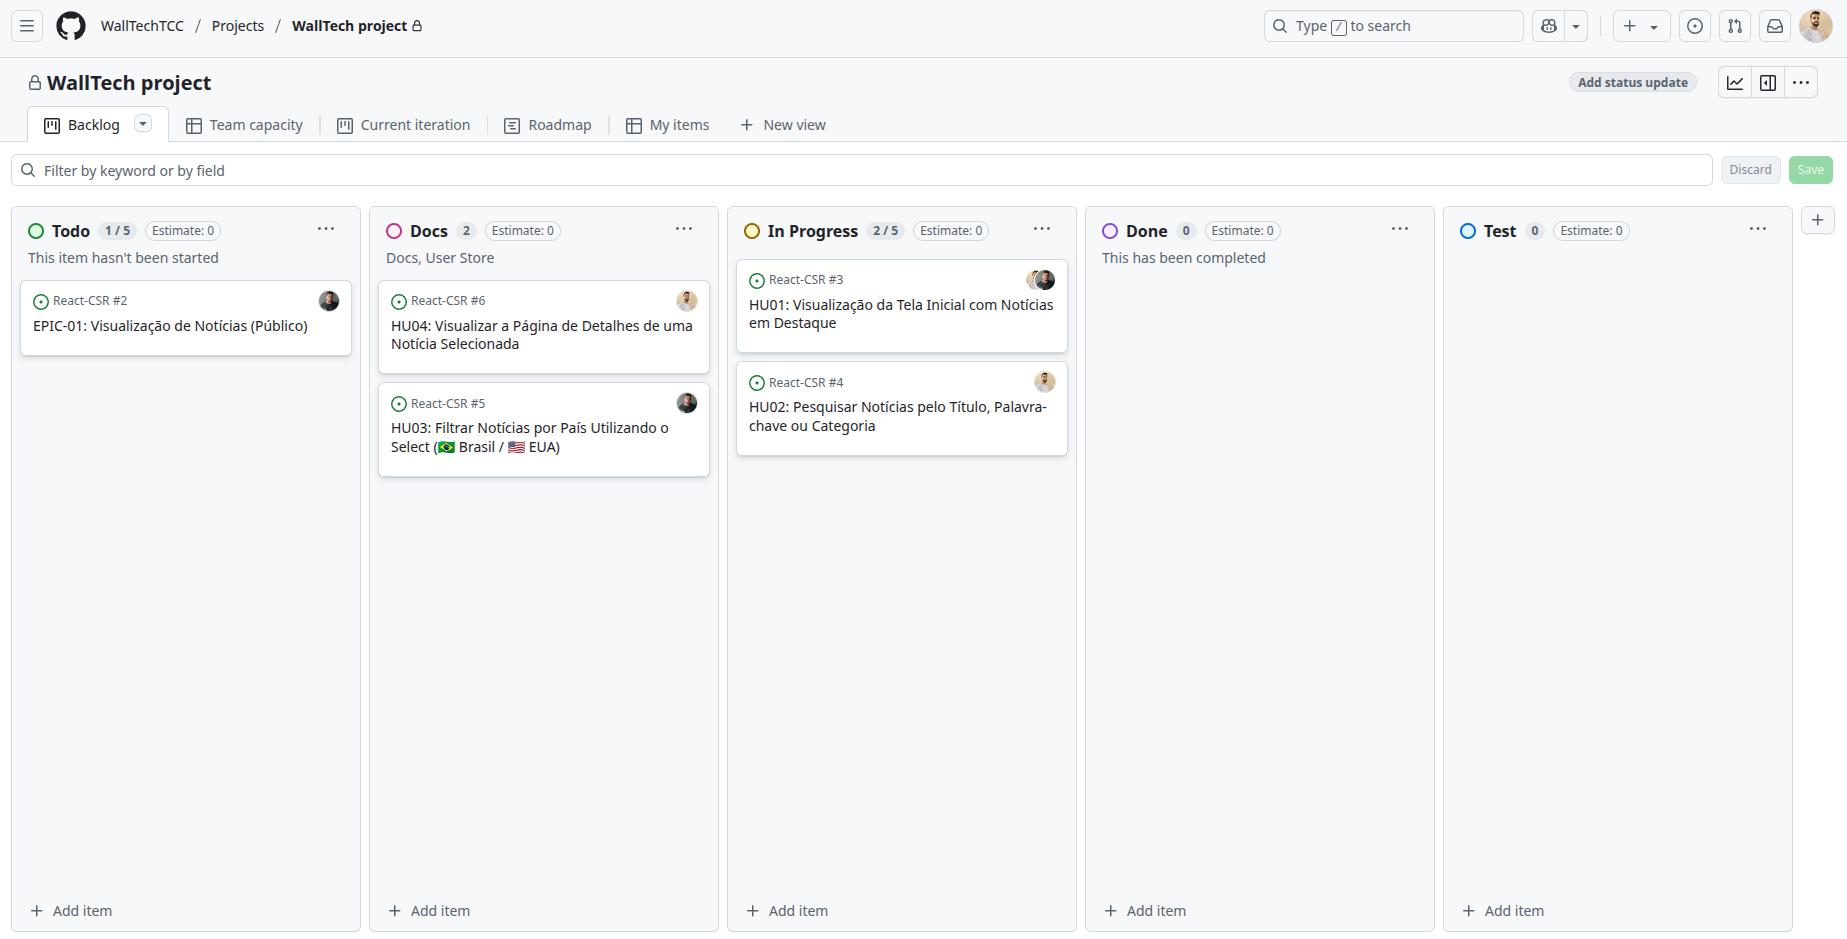
\includegraphics[width=1.0\textwidth]{media/wall_tech_kanban.png}
  \legend{Fonte: os autores.}
  \label{fig:kanban-walltech}
\end{figure}

\begin{figure}[H]
  \centering
  \caption{Exemplo de cartão \english{issue} no \english{GitHub Projects}}
  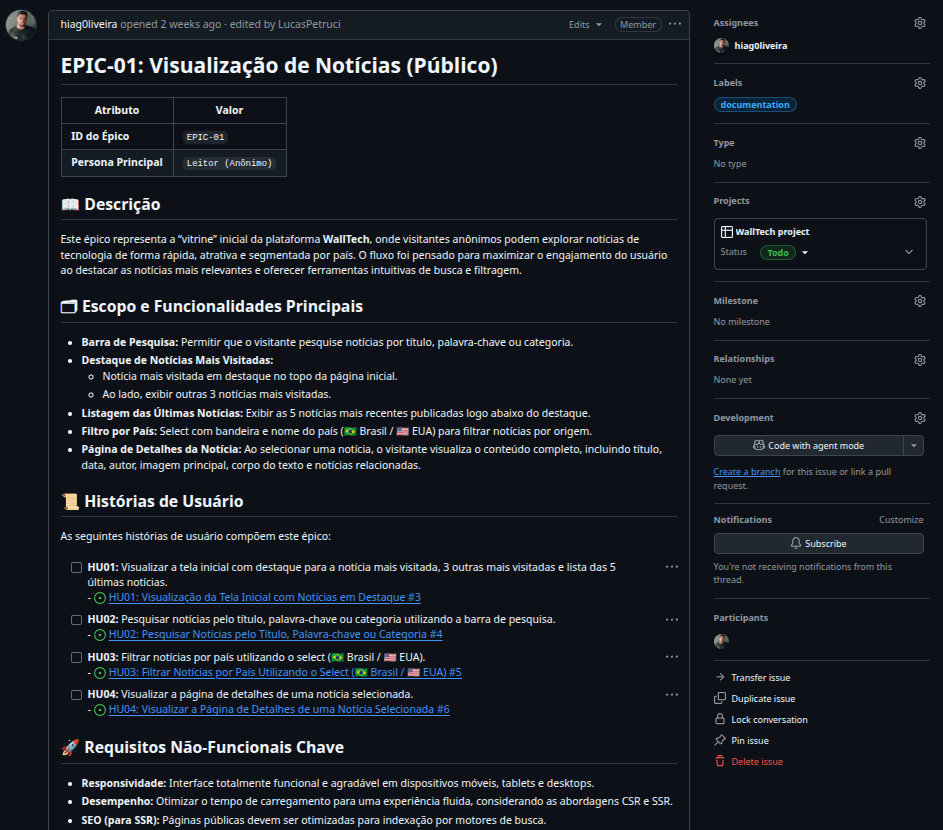
\includegraphics[width=0.7\textwidth]{media/wall_tech_epic.png}
  \legend{Fonte: os autores.}
  \label{fig:kanban-userstories}
\end{figure}




\subsection{Planejamento Funcional: Épico e Histórias de Usuário}

Para guiar o desenvolvimento da plataforma \textbf{WallTech}, foi adotada uma abordagem baseada em práticas ágeis, especialmente no uso de \textit{épicos} e \textit{histórias de usuário}. Essa técnica visa descrever funcionalidades a partir da perspectiva do usuário, proporcionando clareza sobre o propósito e os objetivos de cada componente da aplicação.

As histórias de usuário foram redigidas segundo o modelo dos \textbf{3Ws (Who, What, Why)}, uma técnica comum em análise de requisitos que busca responder:
\begin{itemize}
  \item \textbf{Who (Quem):} Quem está solicitando ou interagindo com a funcionalidade?
  \item \textbf{What (O quê):} Qual é a ação ou funcionalidade desejada?
  \item \textbf{Why (Por quê):} Qual é o benefício ou valor esperado para o usuário?
\end{itemize}

Esse modelo torna a narrativa mais centrada no usuário e contribui para um entendimento compartilhado entre desenvolvedores, designers e partes interessadas. Além disso, as funcionalidades foram agrupadas em \textbf{épicos}, que representam blocos de funcionalidades coesas e de maior escala dentro do sistema.

A seguir, apresenta-se o \textbf{EPIC-01}, responsável por organizar as funcionalidades relacionadas à visualização pública de notícias na plataforma WallTech, seguido de suas respectivas histórias de usuário.

\subsubsection*{EPIC-01: Visualização de Notícias (Público)}

\begin{itemize}
  \item \textbf{ID do Épico:} EPIC-01
  \item \textbf{Persona Principal:} Leitor (Anônimo)
\end{itemize}

\noindent \textbf{Descrição:} Este épico representa a “vitrine” da plataforma WallTech, onde visitantes anônimos podem explorar notícias de tecnologia de forma rápida, atrativa e segmentada por país. O fluxo foi pensado para maximizar o engajamento do usuário ao destacar as notícias mais relevantes e oferecer ferramentas intuitivas de busca e filtragem.

\noindent \textbf{Funcionalidades Principais:}
\begin{itemize}
  \item Barra de pesquisa (por título, palavra-chave ou categoria);
  \item Destaque para a notícia mais visitada e outras três recentemente acessadas;
  \item Listagem das cinco últimas notícias;
  \item Filtro por país (Brasil ou EUA);
  \item Página de detalhes da notícia com conteúdo completo e relacionadas.
\end{itemize}

\noindent \textbf{Requisitos Não-Funcionais:}
\begin{itemize}
  \item Interface responsiva em diferentes dispositivos;
  \item Otimização de desempenho para carregamento rápido;
  \item Suporte a SEO nas páginas públicas (relevante em SSR).
\end{itemize}

\noindent \textbf{Critérios de Aceite:}
\begin{itemize}
  \item Visitantes conseguem navegar e visualizar notícias sem necessidade de login;
  \item É possível realizar pesquisas e aplicar filtros por país;
  \item A navegação é responsiva, intuitiva e eficiente;
  \item A página de detalhes apresenta informações completas da notícia.
\end{itemize}

\subsubsection*{HU01: Visualização da Tela Inicial com Notícias em Destaque}

\begin{itemize}
  \item \textbf{Who:} Visitante anônimo
  \item \textbf{What:} Ver na página inicial uma barra de pesquisa, uma notícia mais visitada em destaque, três outras recém acessadas e uma lista com as cinco últimas notícias publicadas.
  \item \textbf{Why:} Explorar rapidamente o conteúdo mais relevante e recente sobre tecnologia.
\end{itemize}

\noindent \textbf{História:} \textit{Como um visitante, quero ver na página inicial uma barra de pesquisa, a notícia mais visitada em destaque, outras três recém visitadas ao lado e as cinco últimas notícias abaixo, para que eu possa explorar rapidamente o conteúdo mais relevante sobre tecnologia.}

\noindent \textbf{Critérios de Aceite:}
\begin{itemize}
  \item A página inicial contém uma barra de pesquisa funcional;
  \item A notícia mais visitada aparece em destaque;
  \item Outras três notícias aparecem ao lado da principal;
  \item Abaixo, as cinco últimas notícias são exibidas em ordem cronológica;
  \item Interface é responsiva e com bom desempenho.
\end{itemize}

\subsubsection*{HU02: Pesquisar Notícias por Palavra-chave ou Categoria}

\begin{itemize}
  \item \textbf{Who:} Visitante
  \item \textbf{What:} Utilizar a barra de pesquisa para buscar por título, palavra-chave ou categoria.
  \item \textbf{Why:} Encontrar conteúdos relevantes de forma eficiente.
\end{itemize}

\noindent \textbf{História:} \textit{Como um visitante, quero pesquisar notícias por título, palavra-chave ou categoria, para que eu possa encontrar facilmente conteúdos relevantes sem precisar navegar por toda a lista.}

\noindent \textbf{Critérios de Aceite:}
\begin{itemize}
  \item Campo de texto para busca;
  \item Filtro por categoria;
  \item Resultados relevantes são exibidos com base na busca;
  \item A busca pode ser combinada com o filtro por categoria;
  \item Mensagem amigável exibida em caso de nenhum resultado.
\end{itemize}

\subsubsection*{HU03: Filtrar Notícias por País}

\begin{itemize}
  \item \textbf{Who:} Visitante
  \item \textbf{What:} Filtrar as notícias por país usando um seletor com bandeiras.
  \item \textbf{Why:} Visualizar conteúdos específicos da localidade desejada.
\end{itemize}

\noindent \textbf{História:} \textit{Como um visitante, quero filtrar notícias por país (Brasil ou EUA), para que eu possa visualizar apenas conteúdos relevantes para minha localidade ou interesse regional.}

\noindent \textbf{Critérios de Aceite:}
\begin{itemize}
  \item Menu com seleção de país exibindo bandeira e nome;
  \item Lista de notícias é atualizada dinamicamente conforme a seleção;
  \item O filtro mantém o estado ao navegar;
  \item Filtro compatível com busca por palavra-chave ou categoria.
\end{itemize}

\subsubsection*{HU04: Visualizar Detalhes de uma Notícia}

\begin{itemize}
  \item \textbf{Who:} Visitante
  \item \textbf{What:} Acessar a página de detalhes de uma notícia específica.
  \item \textbf{Why:} Ler o conteúdo completo e visualizar informações adicionais.
\end{itemize}

\noindent \textbf{História:} \textit{Como um visitante, quero clicar em uma notícia para acessar sua página de detalhes, para que eu possa ler o conteúdo completo e visualizar informações relacionadas.}

\noindent \textbf{Critérios de Aceite:}
\begin{itemize}
  \item Acesso a uma URL única da notícia;
  \item Exibição completa do conteúdo (título, autor, data, imagem, corpo do texto, país de origem);
  \item Exibição de até três notícias relacionadas;
  \item Página de erro amigável no caso de URL inválida;
  \item Botão para retornar à lista ou pesquisa anterior.
\end{itemize}









\section{Requisitos}
\label{section:requisitos}

O levantamento e a definição dos requisitos da plataforma \textbf{WallTech} foram guiados pelas necessidades dos usuários e organizados por meio da técnica de \textit{histórias de usuário}, agrupadas em \textit{épicos}. A partir da análise funcional do \textbf{EPIC-01 — Visualização de Notícias (Público)}, foram identificadas as principais funcionalidades esperadas para a aplicação, considerando tanto o fluxo de interação do visitante quanto os objetivos de usabilidade, desempenho e escalabilidade.

Os requisitos a seguir foram organizados em duas categorias: \textbf{funcionais}, que representam as funcionalidades diretamente percebidas pelos usuários, e \textbf{não funcionais}, que tratam de atributos como desempenho, acessibilidade e responsividade.

\subsection{Requisitos Funcionais}
\label{subsec:requisitos-funcionais}

\begin{itemize}
  \item O sistema deve permitir que visitantes visualizem uma lista de notícias recentes e em destaque.
  \item O sistema deve disponibilizar uma barra de pesquisa por palavra-chave, título ou categoria.
  \item O sistema deve permitir a filtragem de notícias por país (🇧🇷 Brasil ou 🇺🇸 EUA).
  \item O sistema deve possibilitar o acesso aos detalhes completos de uma notícia selecionada.
  \item O sistema deve armazenar localmente os acessos recentes para melhorar a experiência do usuário.
  \item O sistema deve apresentar mensagens claras em situações de ausência de conteúdo.
\end{itemize}

\subsection{Requisitos Não Funcionais}
\label{subsec:requisitos-nao-funcionais}

\begin{itemize}
  \item A interface deve ser responsiva, adaptando-se corretamente a diferentes tamanhos de tela.
  \item O carregamento das páginas deve ser otimizado, proporcionando uma experiência fluida mesmo em conexões lentas.
  \item O sistema deve estar preparado para indexação por motores de busca (SEO), quando aplicado via Server-Side Rendering.
  \item A navegação deve ser acessível, com suporte a teclado e leitores de tela.
  \item A interface deve manter a consistência visual e funcional entre suas versões SPA e MPA.
\end{itemize}




\section{Design do Sistema}
\label{cap:design}

O design do sistema foi orientado para refletir as diferenças estruturais entre as abordagens \acrshort{spa} e \acrshort{mpa}, levando em consideração os requisitos funcionais da plataforma \textit{WallTech}. Esta vitrine digital exibe notícias de tecnologia obtidas por meio da \textit{NewsAPI}, com recursos de busca, filtragem e destaque de conteúdo segmentado por país. Não há backend próprio, sendo todas as chamadas feitas diretamente para a API externa, o que simplifica a arquitetura e acentua o papel do frontend na renderização de conteúdo.

Para modelagem arquitetural e comportamental, foram utilizados diagramas da UML, incluindo:
\begin{itemize}
  \item \textbf{Diagrama de Caso de Uso}, para representar as principais funcionalidades acessadas pelos usuários visitantes.
  \item \textbf{Diagrama de Sequência}, a fim de ilustrar o fluxo de interação entre navegador e a \textit{NewsAPI} durante operações como busca e carregamento de notícias.
  \item \textbf{Diagrama de Componentes}, para representar os módulos da aplicação, como a interface, o serviço de requisição à API, e os componentes de renderização.
\end{itemize}

As decisões de design foram fundamentadas em boas práticas para renderização web discutidas por \cite{osmani2025}, bem como nas diretrizes da literatura especializada em arquitetura de frontend, como apresentado pela \cite{atori2024}.

Segundo \cite{osmani2025}, a escolha entre renderização no cliente ou no servidor deve considerar o contexto da aplicação, os requisitos de desempenho e os objetivos de SEO. Já o artigo da \cite{atori2024} destaca que SPAs tendem a oferecer maior fluidez e interatividade, enquanto MPAs são mais eficazes em aplicações que dependem de indexação e acessibilidade.

\section{Abordagens de Renderização e Navegação}
\label{section:abordagens-renderizacao}

Para o estudo comparativo, a plataforma foi desenvolvida em duas arquiteturas distintas de renderização e navegação: 
\acrfull{ssr} com \acrfull{mpa} e \acrfull{csr} com \acrfull{spa}.  
Cada abordagem foi implementada com tecnologias adequadas ao seu paradigma Next.js para \acrshort{ssr}/\acrshort{mpa} e React para \acrshort{csr}/\acrshort{spa}  permitindo observar diferenças de desempenho, interatividade e otimização para mecanismos de busca (\acrshort{seo}).

A seguir, cada abordagem é apresentada com seu fluxo típico de funcionamento, diagrama de componentes (representando a estrutura modular) e diagrama de sequência (detalhando as interações passo a passo).

\subsection{SSR/MPA - Fluxo e Arquitetura}
\label{subsec:ssr-mpa}

Na abordagem \acrfull{ssr} com \acrfull{mpa}, cada página é renderizada no servidor a partir de uma requisição HTTP completa. O HTML final já é entregue com os dados integrados, permitindo que o navegador exiba o conteúdo imediatamente, favorecendo o tempo de carregamento inicial e a indexação por \textit{crawlers} \cite{atori2024}.

\begin{itemize}
  \item O \textbf{usuário} acessa o site;
  \item O \textbf{navegador} envia uma requisição \texttt{GET} ao \textbf{servidor Next.js};
  \item O servidor obtém os dados mais recentes na \textbf{NewsAPI};
  \item O servidor monta a página HTML já com os dados;
  \item O HTML é enviado ao navegador e exibido;
  \item Cada navegação subsequente gera nova requisição completa ao servidor;
  \item Scripts no cliente utilizam \textbf{LocalStorage} para melhorar a experiência.
\end{itemize}
  
A Figura \ref{fig:component-diagram-next} ilustra como, nesta arquitetura, o \textbf{navegador} interage diretamente com o \textbf{Servidor Next.js} para cada página requisitada. O servidor, por sua vez:
\begin{enumerate}
  \item Identifica a rota usando o \textbf{roteamento baseado em arquivos};
  \item Executa a lógica de busca de dados (\texttt{getServerSideProps});
  \item Faz chamadas à \textbf{NewsAPI} para obter o conteúdo;
  \item Renderiza o HTML e o envia ao cliente.
\end{enumerate}

A Figura \ref{fig:sequence-diagram-ssr} detalha a ordem das interações. O usuário inicia a navegação, o servidor processa a requisição, consulta a API externa, renderiza o HTML e envia a resposta pronta para o cliente. O uso de \textit{hydration} ativa a interatividade após o carregamento inicial.

\begin{figure}[H]
  \centering
  \caption{Diagrama de sequência - \acrshort{ssr}/\acrshort{mpa}}
  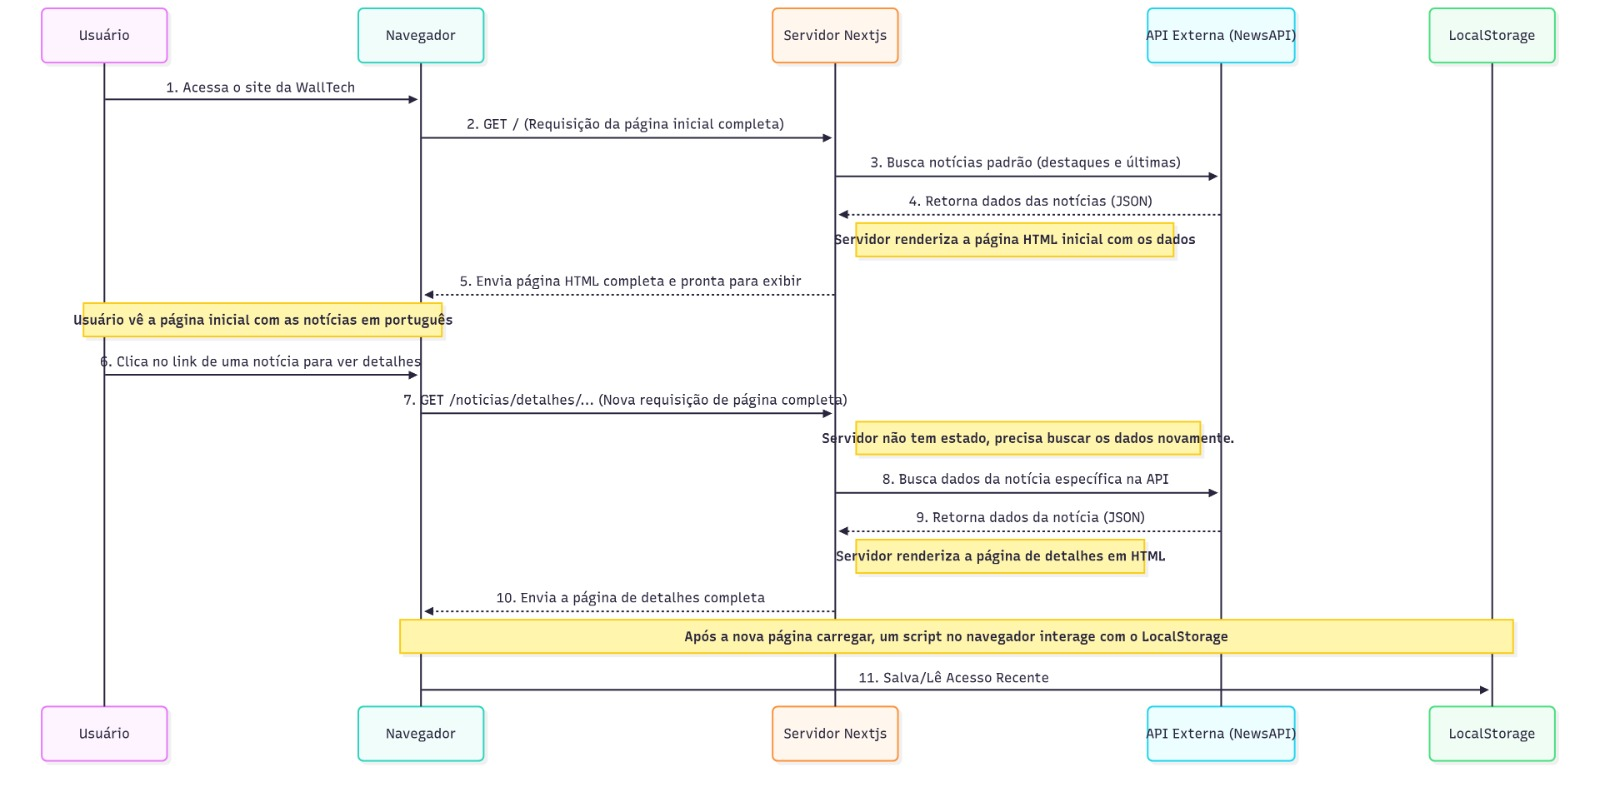
\includegraphics[width=1\textwidth]{media/wall_tech_sequence_diagram.jpeg}
  \legend{Fonte: os autores.}
  \label{fig:sequence-diagram-ssr}
\end{figure}


A Figura \ref{fig:component-diagram-next} mostra que, nessa arquitetura, o \textbf{servidor Next.js} centraliza o roteamento, a obtenção de dados e a renderização das páginas, entregando ao navegador HTML já pré-renderizado. Após o carregamento, scripts ativam a interatividade e permitem o uso do \textbf{LocalStorage}.

\begin{figure}[H]
  \centering
  \caption{Diagrama de Componentes - \acrshort{mpa} (\acrshort{ssr} em Next.js)}
  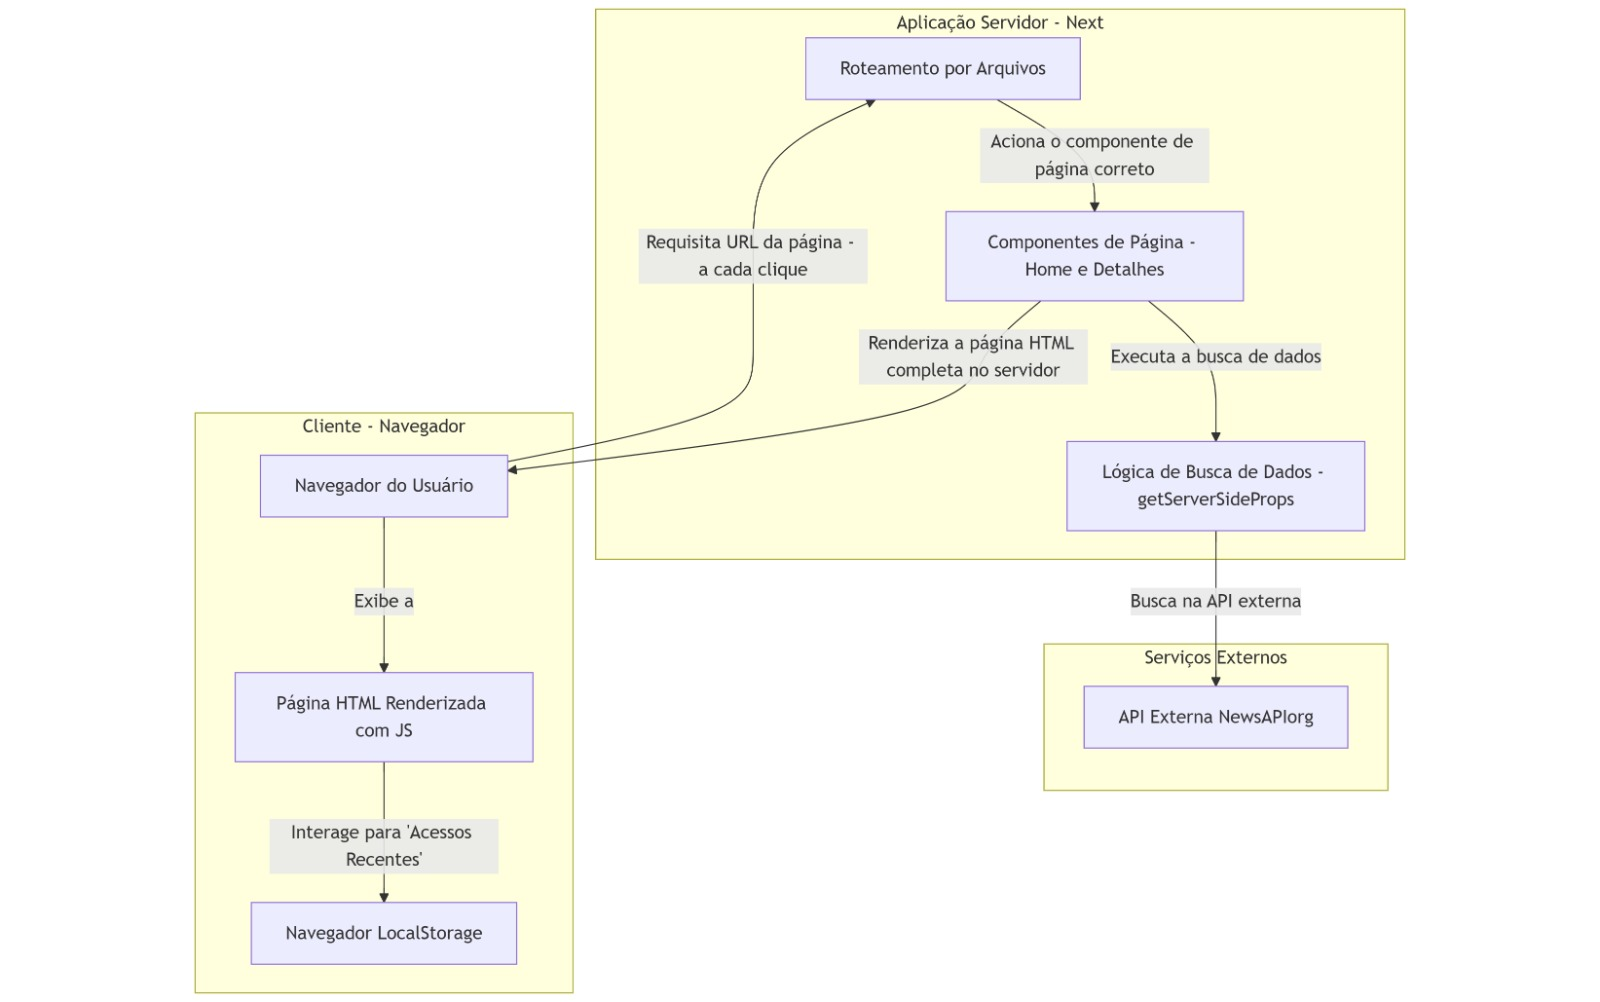
\includegraphics[width=1\textwidth]{media/component-diagram-next.jpeg}
  \legend{Fonte: os autores.}
  \label{fig:component-diagram-next}
\end{figure}


\subsection{CSR/SPA - Fluxo e Arquitetura}
\label{subsec:csr-spa}

Na abordagem \acrfull{csr} com \acrfull{spa}, o carregamento inicial envia um HTML mínimo e um pacote JavaScript que contém toda a lógica da aplicação. A partir daí, a navegação e renderização são executadas no navegador, sem recarregar a página.

\begin{itemize}
  \item O \textbf{usuário} acessa o site;
  \item O navegador baixa o \textbf{bundle React} e monta a interface inicial;
  \item O \textbf{gerenciador de estado} solicita dados à \textbf{NewsAPI};
  \item A interface é atualizada dinamicamente com os dados recebidos;
  \item Ao navegar, o \textbf{roteador do React} altera a URL e renderiza novos componentes;
  \item Dados podem ser lidos ou salvos no \textbf{LocalStorage}.
\end{itemize}

A Figura \ref{fig:sequence-diagram-csr} descreve como o navegador processa as interações: primeiro carrega a aplicação, depois solicita dados conforme necessário e atualiza a interface sem recarregar a página, garantindo uma navegação contínua.

\begin{figure}[H]
  \centering
  \caption{Diagrama de sequência - \acrshort{csr}/\acrshort{spa}}
  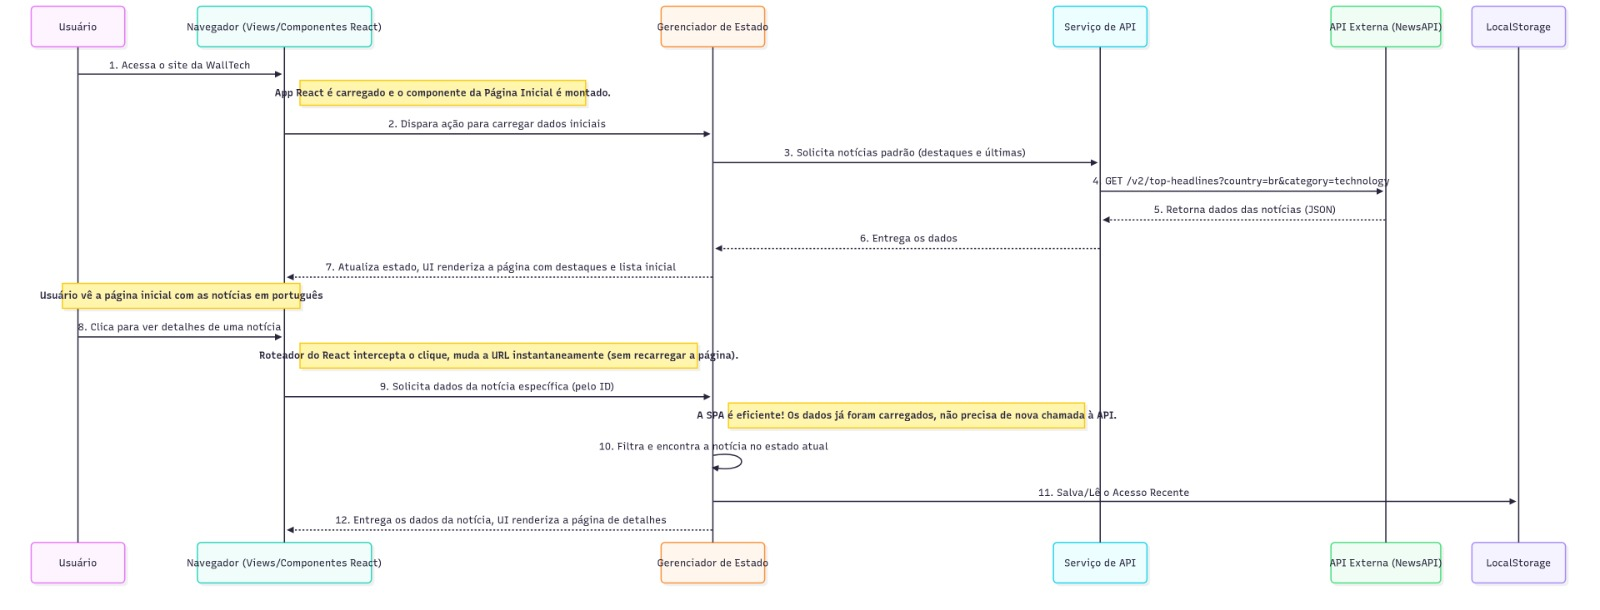
\includegraphics[width=1\textwidth]{media/wall_tech_detail_sequence_diagram.jpeg}
  \legend{Fonte: os autores.}
  \label{fig:sequence-diagram-csr}
\end{figure}


A Figura \ref{fig:component-diagram-react} mostra que, nessa arquitetura, o navegador concentra toda a lógica de renderização. O \textbf{Roteador React} decide quais componentes de página serão exibidos, enquanto o \textbf{Gerenciador de Estado} controla o fluxo de dados entre a interface e a \textbf{NewsAPI}.

\begin{figure}[H]
  \centering
  \caption{Diagrama de Componentes - \acrshort{spa} (React)}
  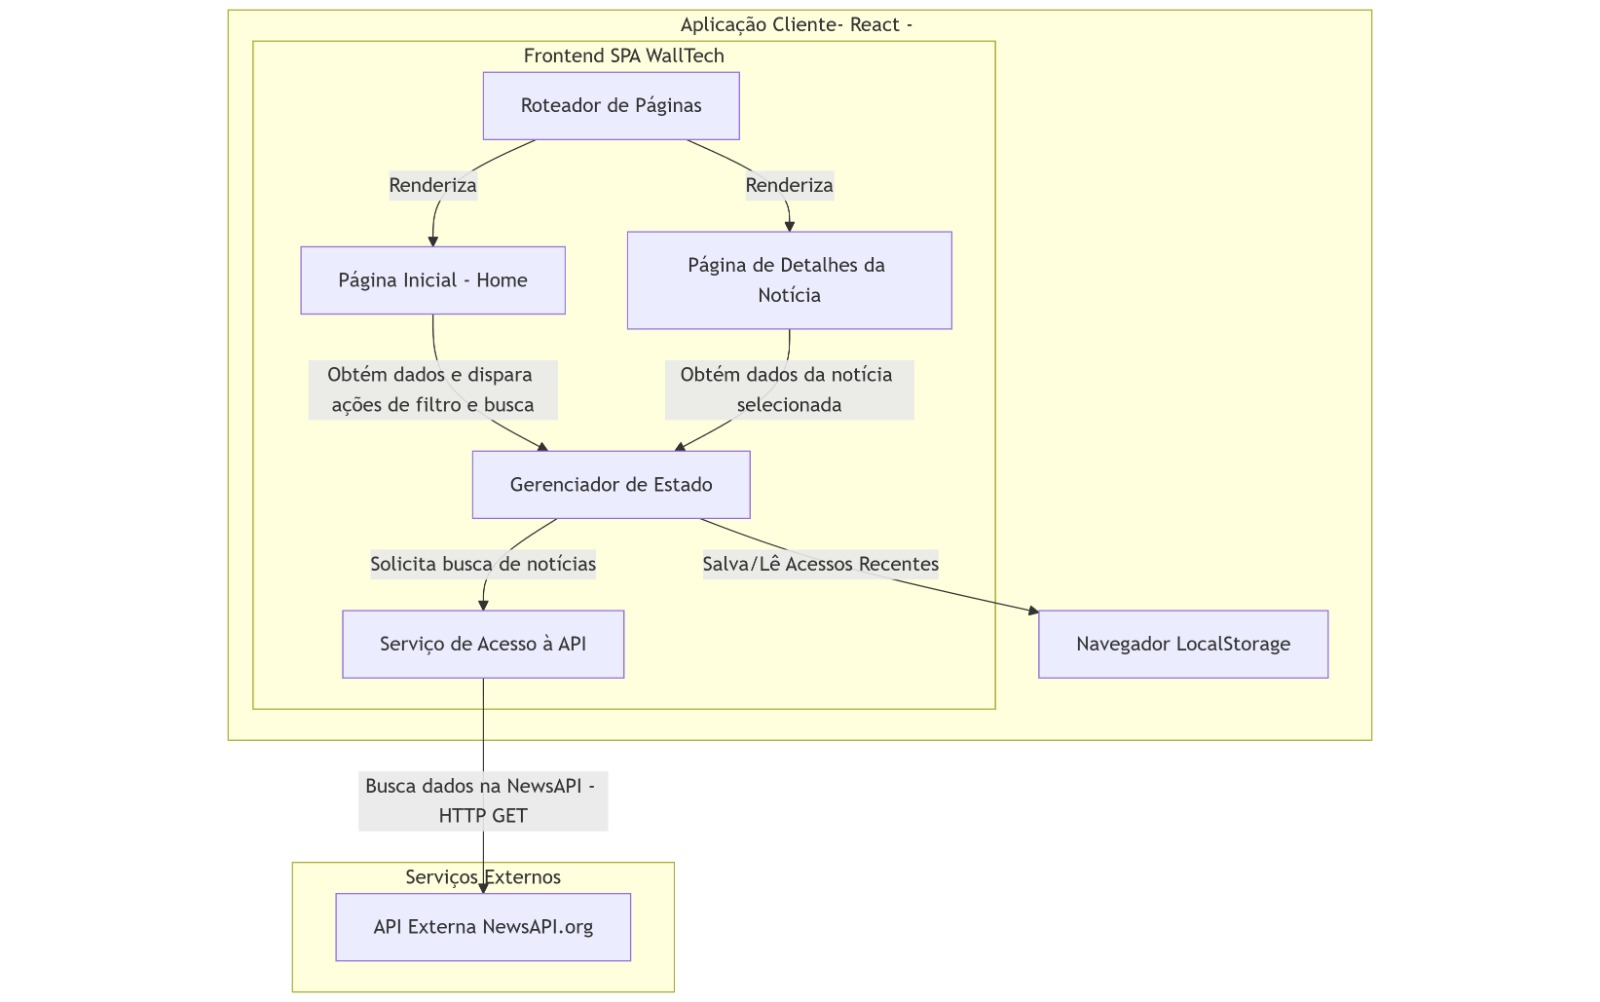
\includegraphics[width=1\textwidth]{media/component-diagram-react.jpeg}
  \legend{Fonte: os autores.}
  \label{fig:component-diagram-react}
\end{figure}



\section{Implementação}
\label{sec:implementacao}

Esta seção descreve o conjunto de tecnologias, bibliotecas e ferramentas que são empregadas para a construção das duas versões do sistema de prova de conceito, detalhando a fundamentação para a escolha de cada componente do ecossistema de desenvolvimento. O gerenciamento do código-fonte e do ciclo de vida do projeto é realizado com o sistema de controle de versão \textbf{Git} e a plataforma de hospedagem \textbf{GitHub}, conforme as práticas descritas na Seção~\ref{sec:git-github}.

Ambas as implementações consomem dados da mesma fonte externa, a \textbf{News API}, uma \acrshort{api} RESTful que fornece o conteúdo jornalístico para a aplicação, como detalhado na Seção~\ref{sec:news-api}. Para garantir a consistência visual e a qualidade da interface entre as duas arquiteturas, utiliza-se a biblioteca de componentes \textbf{shadcn/ui}, que oferece um conjunto de componentes acessíveis e personalizáveis, conforme apresentado na Seção~\ref{sec:ferramentas-modernas}.

\subsection{Implementação da Aplicação SPA}
\label{ssec:implementacao_spa}

A implementação da \acrfull{spa} é desenvolvida utilizando a biblioteca \textbf{React} na sua versão 18. O React é uma biblioteca JavaScript declarativa, mantida pela Meta, focada na construção de interfaces de usuário a partir de componentes reutilizáveis. Sua adoção neste projeto se dá por sua vasta popularidade no mercado e ao seu paradigma de componentização, que facilita a criação de UIs modulares e de fácil manutenção \cite{react2025}. A eficiência da renderização é otimizada pelo uso de um DOM Virtual, um conceito central da biblioteca que minimiza as manipulações diretas no navegador.

Para a estruturação inicial do projeto e o gerenciamento do ambiente de desenvolvimento, utiliza-se a ferramenta de \textit{build} \textbf{Vite}. O Vite é um ecossistema de desenvolvimento frontend moderno que oferece um servidor de desenvolvimento com recarregamento rápido (\textit{Hot Module Replacement}) e um processo de compilação (\textit{build}) otimizado, que resulta em pacotes de produção menores e mais eficientes \cite{vite_docs}.

O roteamento no lado do cliente, uma característica fundamental da arquitetura SPA, implementa-se com a biblioteca \textbf{React Router}. Trata-se da solução padrão para navegação em aplicações React, que possibilita a criação de uma experiência de usuário fluida e sem recarregamentos de página ao manipular a \acrshort{api} de Histórico do navegador \cite{react_router_docs}. A comunicação com a News API é realizada por meio da \acrshort{api} \texttt{fetch}, nativa dos navegadores modernos.

A \autoref{fig:app-react-csr} mostra a \textbf{página inicial} da plataforma WallTech na implementação \acrshort{spa} com \acrshort{csr}, em conformidade com o wireframe (\autoref{fig:wireframe-walltech}). Nessa página, o usuário visualiza a notícia mais visitada em destaque, três outras recentemente acessadas ao lado, uma lista com as cinco últimas notícias publicadas, além de barra de pesquisa e filtro por país (Brasil ou EUA).

\begin{figure}[H]
  \centering
  \caption{Aplicação SPA com React (\acrshort{csr})}
  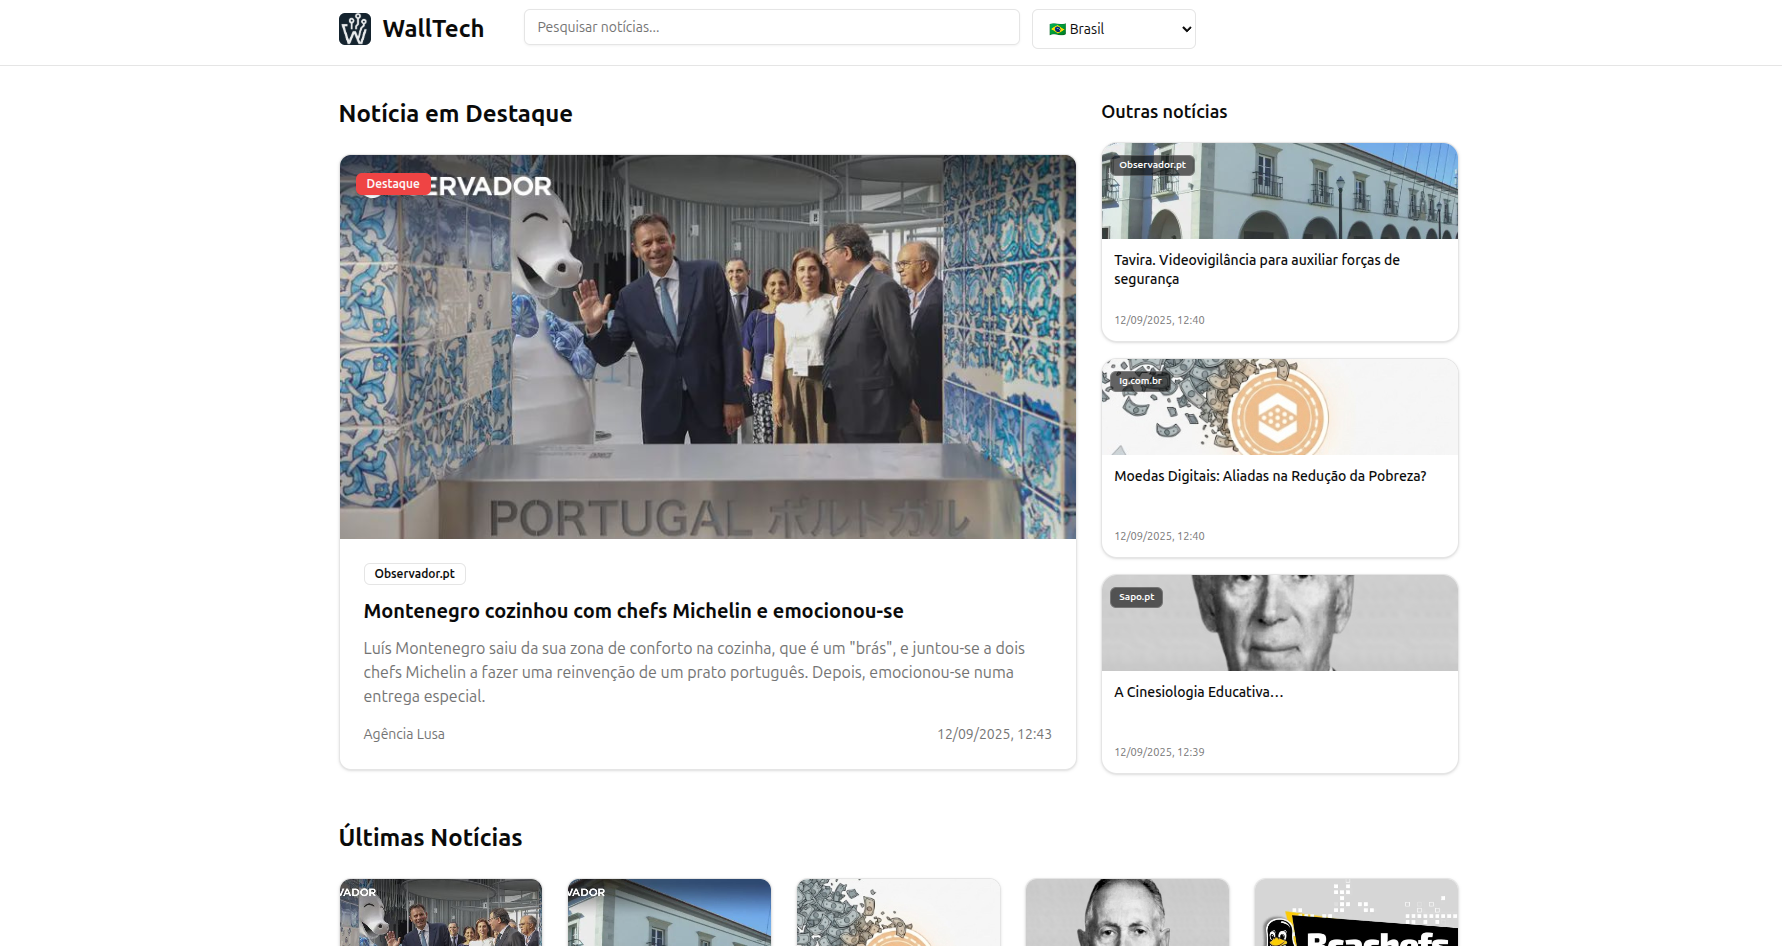
\includegraphics[width=0.9\textwidth]{media/app_react_csr.png}
  \legend{Fonte: os autores.}
  \label{fig:app-react-csr}
\end{figure}

\subsection{Implementação da Aplicação MPA}
\label{ssec:implementacao_mpa}

A implementação da \acrfull{mpa}, com foco em \acrfull{ssr}, é desenvolvida com o \emph{framework} \textbf{Next.js} na versão 14. O Next.js é um meta-framework baseado em React, mantido pela Vercel, que se posiciona como uma solução completa para a construção de aplicações web de produção. Sua escolha para este estudo de caso justifica-se por ser a principal referência de mercado para a implementação de \acrshort{ssr} no ecossistema React, oferecendo uma estrutura robusta e opinativa \cite{nextjs2024}.

O \emph{framework} opera sobre um ambiente \textbf{Node.js}, o que permite a execução de código JavaScript no lado do servidor \cite{nodejs2025}. Essa capacidade é a base da renderização no servidor, onde o Next.js utiliza funções específicas, como a \texttt{getServerSideProps}, para buscar dados de fontes externas e pré-renderizar o HTML completo de uma página antes de enviá-la ao navegador. Além disso, o Next.js implementa um sistema de roteamento baseado no sistema de arquivos, onde a estrutura de diretórios da pasta \texttt{pages} define automaticamente as rotas da aplicação, simplificando a configuração e a manutenção do projeto.


A \autoref{fig:app-next-ssr} mostra a \textbf{página de detalhes} de uma notícia na plataforma WallTech, na implementação \acrshort{mpa} com \acrshort{ssr}. Ao clicar em uma notícia na listagem, o usuário é direcionado para esta tela, onde pode visualizar imagem, fonte, título, metadados (agência e data/hora) e resumo. Também é possível acessar a matéria original pelo botão “Ler na fonte” e retornar à página anterior pelo botão “Voltar”.

\begin{figure}[H]
  \centering
  \caption{Aplicação MPA com Next.js (\acrshort{ssr})}
  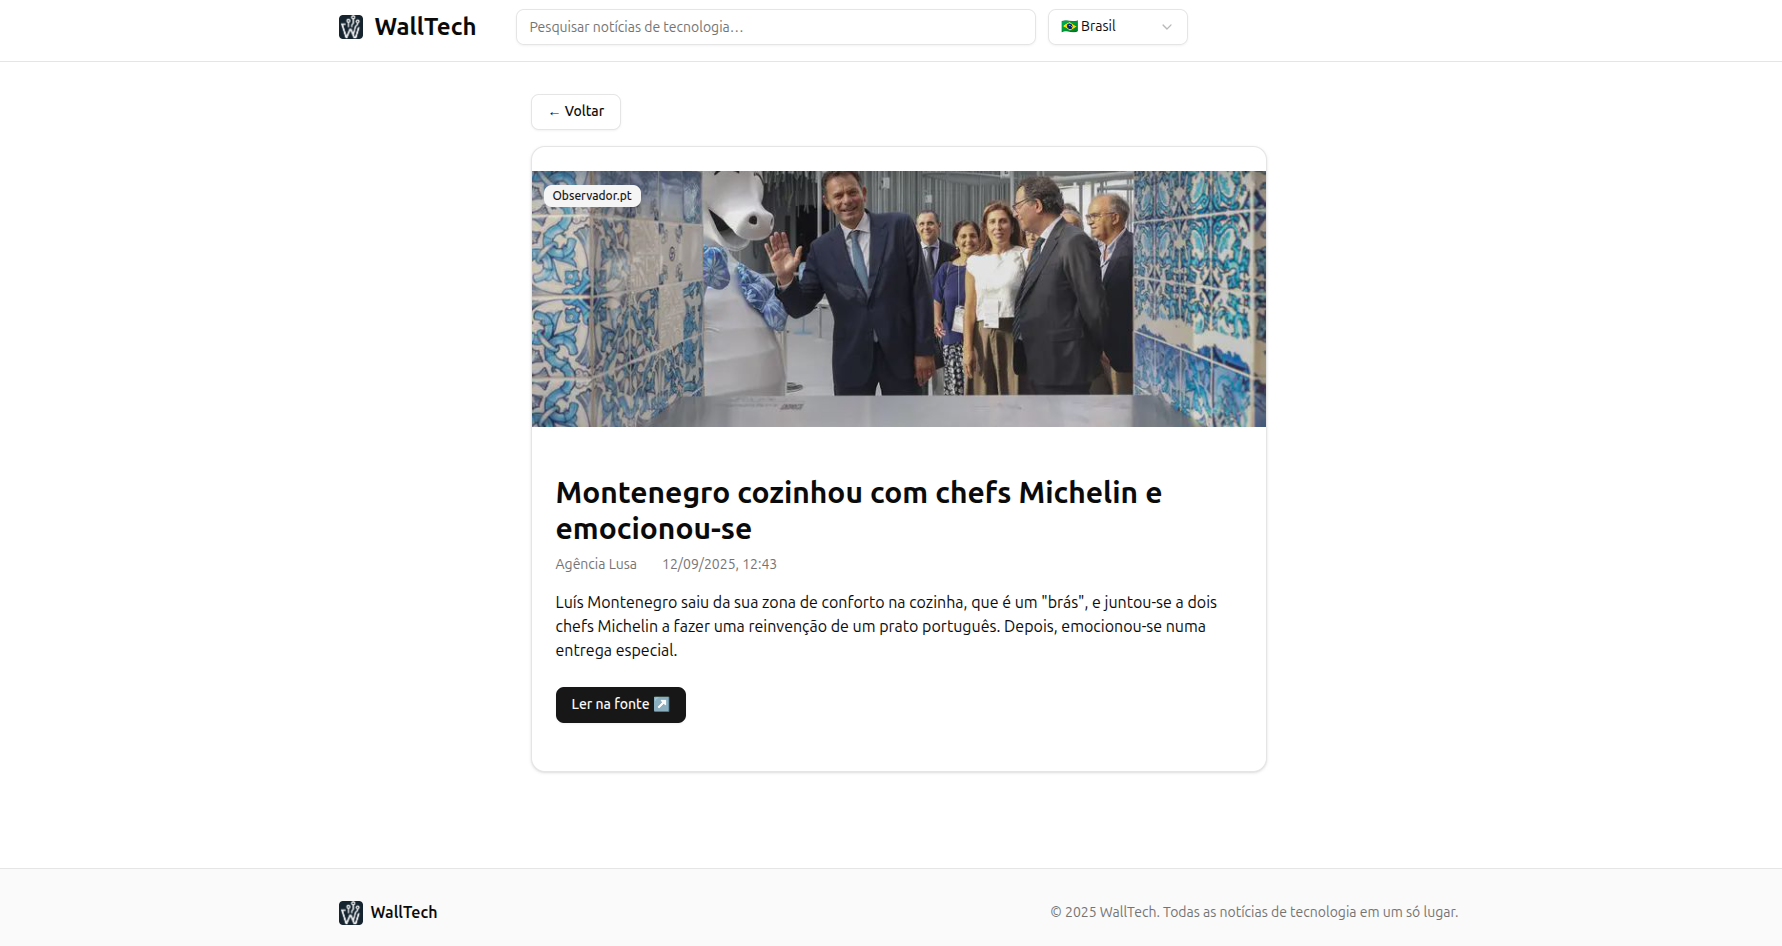
\includegraphics[width=0.9\textwidth]{media/app_next_ssr.png}
  \legend{Fonte: os autores.}
  \label{fig:app-next-ssr}
\end{figure}



\vspace{1cm}
Com as duas versões da plataforma WallTech implementadas e funcionais, o alicerce para a análise comparativa foi estabelecido. O capítulo seguinte detalha a metodologia experimental rigorosa empregada para a execução dos testes, a configuração do ambiente controlado e os procedimentos de coleta de dados, garantindo que a comparação entre as abordagens \acrshort{csr} e \acrshort{ssr} seja justa, precisa e reprodutível.



\chapter{Coleta de Dados}
\label{cap:metodologia_experimental}

Após o desenvolvimento das duas versões da plataforma WallTech, este capítulo descreve os procedimentos metodológicos adotados para conduzir a análise de desempenho comparativa. O objetivo aqui é detalhar o ambiente de testes controlado, as ferramentas de instrumentação para coleta de métricas, o processo de empacotamento das aplicações e os protocolos de execução. A adoção de um rigor metodológico é fundamental para assegurar a validade, a confiabilidade e a reprodutibilidade dos dados que serão apresentados e discutidos no capítulo de Resultados.



\section{Configuração do Ambiente Experimental}
\label{sec:ambiente-experimental}

Esta seção detalha como as duas versões da plataforma \textbf{WallTech} uma \acrshort{mpa} com \acrshort{ssr} (Next.js) e uma \acrshort{spa} com \acrshort{csr} (React+Vite) foram instrumentadas para coleta de \textit{Web Vitals}, empacotadas em contêineres \textit{Docker} com \textbf{paridade de recursos} e executadas em ambiente \textbf{local controlado} para assegurar reprodutibilidade do estudo.

\subsection{Limitações de Execução e Decisão Metodológica}
\label{ssec:limitacoes-execucao}

Durante o desenvolvimento, a \textit{NewsAPI} impôs restrições de uso em produção (por exemplo, políticas de CORS e/ou limitações do plano vigentes no período do estudo), o que impactaria a coleta de dados em ambiente hospedado. Para \textbf{eliminar interferências externas} e garantir \textbf{controle experimental}, decidiu-se executar ambos os protótipos \textbf{localmente} em contêineres \textit{Docker}, com os \textbf{mesmos limites de CPU e memória}, sistema de arquivos \textit{read-only} e partições temporárias (\textit{tmpfs}) para reduzir variações de I/O. Assim, a comparação \acrshort{csr}~vs.~\acrshort{ssr} foca no \textit{modelo de renderização} e não em diferenças de \textit{hosting}.

\subsection{Instrumentação de Web Vitals}
\label{ssec:instrumentacao-webvitals}

Em ambos os protótipos, a instrumentação é realizada \textbf{no cliente}, e os dados são enviados para um \textbf{endpoint interno} exposto pelo próprio contêiner. Utiliza-se \texttt{navigator.sendBeacon} como via principal (por não bloquear a navegação) e \texttt{fetch} como \textit{fallback} com \texttt{keepalive}. As métricas coletadas são os \textit{Core Web Vitals} atuais: \textbf{TTFB}, \textbf{FCP}, \textbf{LCP}, \textbf{CLS} e \textbf{INP}. 

Os registros são persistidos em \textbf{NDJSON} (uma linha por métrica), contendo, dentre outros, os campos:
\texttt{\{id, name, value, rating, navigationType, attribution, entries, ts\}}. A análise estatística (p.\,ex., \textbf{p50}/\textbf{p95}) está \textit{deliberadamente breve} aqui e será desenvolvida em capítulos posteriores.

\subsubsection{SSR/MPA (Next.js).}
Na versão \acrshort{ssr} (App Router), um \textit{Client Component} global usa \texttt{useReportWebVitals} para escutar e enviar as métricas ao endpoint \texttt{/api/vitals}. No servidor, a rota grava o NDJSON em um caminho configurável: por padrão \texttt{/tmp/webvitals.ndjson} (partição \textit{tmpfs}), ou no caminho definido por \texttt{\$METRICS\_PATH} quando se deseja persistência via volume.

\begin{lstlisting}[language=TypeScript,caption={Endpoint de métricas no SSR/Next.js (visão de servidor)}]
// src/app/api/vitals/route.ts
import { NextRequest, NextResponse } from "next/server";
import { appendFile } from "node:fs/promises";

export const runtime = "nodejs";
export const dynamic = "force-dynamic";

const filePath = process.env.METRICS_PATH ?? "/tmp/webvitals.ndjson";

export async function POST(req: NextRequest) {
  const metric = await req.json();
  const doc = { ...metric, ts: new Date().toISOString() };
  await appendFile(filePath, JSON.stringify(doc) + "\n", "utf8");
  return NextResponse.json({ ok: true });
}
\end{lstlisting}

\begin{lstlisting}[language=TypeScript,caption={Envio de métricas no cliente (SSR/Next.js)}]
"use client";
import { useReportWebVitals } from "next/web-vitals";
import { useCallback } from "react";

export default function WebVitals() {
  const report = useCallback((metric: any) => {
    const body = JSON.stringify({
      id: metric.id, name: metric.name, value: metric.value,
      rating: metric.rating, navigationType: metric.navigationType,
      attribution: metric.attribution, entries: metric.entries, ts: Date.now(),
    });

    if (navigator.sendBeacon) {
      navigator.sendBeacon("/api/vitals",
        new Blob([body], { type: "application/json" }));
    } else {
      fetch("/api/vitals", {
        method: "POST", body, keepalive: true,
        headers: { "Content-Type": "application/json" },
      });
    }
  }, []);

  useReportWebVitals(report);
  return null;
}
\end{lstlisting}

\subsubsection{CSR/SPA (React+Vite).}
Na versão \acrshort{csr}, a coleta usa \texttt{web-vitals/attribution} (para enriquecer \textit{attribution} em \texttt{LCP}/\texttt{CLS}/\texttt{INP}). O envio é feito para \texttt{/api/web-vitals}. Como não há servidor \textit{framework} (p.\,ex., Next), a aplicação é servida por um \textbf{processo Node.js} simples (\texttt{server.cjs}) que entrega o \texttt{dist/} e expõe o endpoint de métricas, gravando no mesmo esquema (\texttt{/tmp} ou \texttt{\$METRICS\_PATH}).

\begin{lstlisting}[language=TypeScript,caption={Envio de métricas no cliente (CSR/React+Vite)}]
import { useEffect } from "react";
import { onCLS, onINP, onLCP, onFCP, onTTFB, type MetricWithAttribution } from "web-vitals/attribution";

export default function WebVitals() {
  useEffect(() => {
    const report = (m: MetricWithAttribution) => {
      const body = JSON.stringify({
        id: m.id, name: m.name, value: m.value, rating: m.rating,
        navigationType: m.navigationType, attribution: m.attribution,
        entries: m.entries, ts: Date.now(),
      });

      if (navigator.sendBeacon) {
        navigator.sendBeacon("/api/web-vitals",
          new Blob([body], { type: "application/json" }));
      } else {
        fetch("/api/web-vitals", {
          method: "POST", body, keepalive: true,
          headers: { "Content-Type": "application/json" },
        });
      }
    };

    onCLS(report); onINP(report); onLCP(report); onFCP(report); onTTFB(report);
  }, []);

  return null;
}
\end{lstlisting}

\begin{lstlisting}[language=Java,caption={Servidor estático + endpoint (CSR/React+Vite)}]
// server.cjs - Node HTTP simples (serve dist/ e expõe /api/web-vitals)
const http = require("node:http");
const { appendFile, readFile, stat } = require("node:fs/promises");
const { createReadStream } = require("node:fs");
const path = require("node:path");

const PORT = process.env.PORT || 3000;
const DIST = path.join(process.cwd(), "dist");
const METRICS_PATH = process.env.METRICS_PATH || "/tmp/webvitals.ndjson";

const server = http.createServer(async (req, res) => {
  const url = new URL(req.url, `http://${req.headers.host}`);

  if (url.pathname === "/api/web-vitals") {
    if (req.method === "POST") {
      const chunks = []; req.on("data", c => chunks.push(c));
      req.on("end", async () => {
        const json = JSON.parse(Buffer.concat(chunks).toString("utf8") || "{}");
        await appendFile(METRICS_PATH, JSON.stringify({ ...json, ts: Date.now() }) + "\n", "utf8");
        res.writeHead(200, { "Content-Type": "application/json" });
        res.end(JSON.stringify({ ok: true }));
      });
      return;
    }
    if (req.method === "GET") {
      const data = await readFile(METRICS_PATH, "utf8").catch(() => "");
      res.writeHead(200, { "Content-Type": "application/x-ndjson" });
      res.end(data); return;
    }
    res.writeHead(405).end(); return;
  }

  // estático + fallback SPA
  let p = decodeURIComponent(url.pathname);
  if (p === "/") p = "/index.html";
  const file = path.join(DIST, p);
  try {
    const s = await stat(file); if (s.isDirectory()) throw 0;
    createReadStream(file).pipe(res);
  } catch {
    createReadStream(path.join(DIST, "index.html")).pipe(res);
  }
});
server.listen(PORT);
\end{lstlisting}

\subsection{Empacotamento Docker: SSR/MPA (Next.js)}
\label{ssec:ssr-docker}

Para \acrshort{ssr}, adotou-se o \textbf{modo standalone} do Next.js e \textit{multi-stage build}: (i) instalação de dependências, (ii) \textit{build} e (iii) \textit{runner} minimalista. O contêiner expõe a porta \texttt{3000}, roda como usuário \texttt{node} e lê variáveis em tempo de execução (importante para segredos e chaves).

\begin{lstlisting}[language=Dockerfile,caption={Dockerfile da aplicação SSR/MPA (Next.js)}]
# ---------- 1) deps ----------
FROM node:20-alpine AS deps
WORKDIR /app
COPY package*.json ./
RUN npm ci --ignore-scripts

FROM node:20-alpine AS builder
WORKDIR /app
ENV NEXT_TELEMETRY_DISABLED=1
COPY --from=deps /app/node_modules ./node_modules
COPY . .
RUN npm run build

FROM node:20-alpine AS runner
WORKDIR /app
ENV NODE_ENV=production
ENV NEXT_TELEMETRY_DISABLED=1

COPY --from=builder /app/.next/standalone ./
COPY --from=builder /app/public ./public
COPY --from=builder /app/.next/static ./.next/static

USER node
EXPOSE 3000
CMD ["node", "server.js"]
\end{lstlisting}

\begin{lstlisting}[language=bash,caption={Build e execução do container SSR com limites e volume de métricas}]
docker build --no-cache -t next-ssr:prod .

docker run --name next-ssr \
  -p 3001:3000 \
  -e METRICS_PATH=/data/webvitals.ndjson \
  -v "$PWD/metrics:/data:rw" \
  --cpus="1.00" --cpuset-cpus="0" \
  --memory="1g" --memory-swap="1g" \
  --pids-limit=256 \
  --read-only \
  --tmpfs /tmp \
  --tmpfs /app/.next/cache \
  next-ssr:prod
\end{lstlisting}

\subsection{Empacotamento Docker: CSR/SPA (React+Vite)}
\label{ssec:csr-docker}

Para \acrshort{csr}, o \textit{build} é produzido pelo Vite e servido por \texttt{server.cjs}. Diferentemente do \acrshort{ssr}, as variáveis \texttt{VITE\_*} são resolvidas em \textbf{tempo de build}; por isso, a \texttt{.env} é copiada para o estágio \textit{builder} (ou alternativamente injetada com \texttt{--build-arg}). Em execução, o caminho do arquivo de métricas é definido por \texttt{\$METRICS\_PATH}.

\begin{lstlisting}[language=Dockerfile,caption={Dockerfile da aplicação CSR/SPA (React+Vite)}]
# ---------- 1) deps ----------
FROM node:20-alpine AS deps
WORKDIR /app
COPY package*.json ./
RUN npm ci --ignore-scripts

# ---------- 2) build ----------
FROM node:20-alpine AS builder
WORKDIR /app
COPY --from=deps /app/node_modules ./node_modules
COPY . .
# 👇 garante que o Vite leia suas VITE_* do host
COPY .env ./.env
RUN npm run build

# ---------- 3) runner ----------
FROM node:20-alpine AS runner
WORKDIR /app
ENV NODE_ENV=production
ENV TZ=UTC
ENV NODE_OPTIONS=--max-old-space-size=512
COPY --from=builder /app/dist ./dist
COPY server.cjs ./server.cjs
USER node
EXPOSE 3000
CMD ["node", "server.cjs"]
\end{lstlisting}

\begin{lstlisting}[language=bash,caption={Build e execução do container CSR com limites e volume de métricas}]
docker build -t react-csr:prod .

docker run --name react-csr \
  -p 3002:3000 \
  -e METRICS_PATH=/data/webvitals.ndjson \
  -v "$PWD/metrics-csr:/data:rw" \
  --cpus="1.00" --cpuset-cpus="0" \
  --memory="1g" --memory-swap="1g" \
  --pids-limit=256 --read-only --tmpfs /tmp \
  react-csr:prod
\end{lstlisting}

\subsection{Paridade de Recursos, Observabilidade e Procedimento de Coleta}
\label{ssec:paridade-observabilidade}

Para evitar viés de ambiente, ambos os contêineres executam com \textbf{paridade de recursos}: \texttt{--cpus="1.0"}, \texttt{--cpuset-cpus="0"} (fixação na CPU 0), \texttt{--memory="1g"}, \texttt{--memory-swap="1g"}, \texttt{--pids-limit=256}, \texttt{--read-only} e \texttt{--tmpfs /tmp} (arquivo de métricas em memória quando não houver volume). No \acrshort{ssr}, \texttt{/app/.next/cache} é montado em \texttt{tmpfs} para reduzir variações de disco.

Durante os testes, o uso de recursos foi acompanhado com:
\begin{lstlisting}[language=bash]
docker stats next-ssr
docker stats react-csr
\end{lstlisting}
Esse monitoramento fornece CPU\% e memória em tempo real, complementando a coleta de \textit{Web Vitals}. O \textbf{procedimento} adotado foi:
(i) \textit{warm-up} com 2 acessos iniciais à mesma rota para estabilizar caches;
(ii) coleta de 10--15 carregamentos por cenário (janela anônima);
(iii) persistência NDJSON por cenário em volumes distintos (por exemplo, \texttt{./metrics} para \acrshort{ssr} e \texttt{./metrics-csr} para \acrshort{csr}).
A \textbf{análise de métricas} (estatísticas descritivas e percentis como p50 e p95) será apresentada em capítulo específico.

\subsection{Repositórios e Reprodutibilidade}
\label{ssec:repositorios-repro}
O código-fonte, instruções de execução e artefatos de instrumentação estão disponíveis nos repositórios públicos da empresa fictícia \textbf{WallTech}:
\begin{itemize}
  \item \textbf{CSR/SPA (React+Vite)}: \url{https://github.com/WallTechTCC/React-CSR}
  \item \textbf{SSR/MPA (Next.js)}: \url{https://github.com/WallTechTCC/Next-SSR}
\end{itemize}
Esses repositórios permitem reproduzir o experimento localmente com os mesmos limites de CPU/RAM, sistema de arquivos \textit{read-only} e coleta de \textit{Web Vitals} no formato NDJSON, preservando a comparabilidade entre \acrshort{csr} e \acrshort{ssr}.


\subsection{Coleta de CPU/RAM do contêiner e exportação em CSV}
\label{ssec:coleta-host-docker-stats}

Para registrar uso de CPU, memória e número de \textit{PIDs} dos contêineres durante os cenários de teste, foi utilizada a telemetria do próprio Docker via \texttt{docker stats} (sem streaming contínuo). As amostras foram coletadas a cada 1\,s e gravadas em arquivos CSV separados por aplicação, no diretório \texttt{metrics-host/}.

\subsubsection{Colunas dos CSVs.}
Cada linha contém:
\begin{itemize}
  \item \textbf{ts}: timestamp da coleta no host (\texttt{YYYY-MM-DD HH:MM:SS});
  \item \textbf{name}: nome do contêiner;
  \item \textbf{cpu\_perc}: percentual de CPU do contêiner (string com ``\%'' conforme \texttt{docker stats});
  \item \textbf{mem\_usage}: uso de memória reportado (formato humano, ex.: ``123.4MiB / 1.00GiB'');
  \item \textbf{mem\_perc}: percentual de memória (string com ``\%'');
  \item \textbf{pids}: quantidade de processos/threads visíveis ao cgroup do contêiner.
\end{itemize}

\subsubsection{Coleta para o contêiner SSR (\texttt{next-ssr}).}
O comando abaixo cria o diretório de métricas (se não existir) e inicia a captura contínua em \texttt{metrics-host/docker-stats-ssr.csv}:
\begin{lstlisting}[language=bash,caption={Captura de CPU/RAM do contêiner SSR e exportação para CSV}]
mkdir -p metrics-host
(
  echo "ts,name,cpu_perc,mem_usage,mem_perc,pids";
  while true; do
    TS=$(date +"%F %T");
    docker stats --no-stream \
      --format "{{.Name}},{{.CPUPerc}},{{.MemUsage}},{{.MemPerc}},{{.PIDs}}" \
      next-ssr | sed "s/^/$TS,/";
    sleep 1;
  done
) >> metrics-host/docker-stats-ssr.csv
\end{lstlisting}

\subsubsection{Coleta para o contêiner CSR (\texttt{react-csr}).}
De forma análoga, a coleta do contêiner CSR grava em \\ \texttt{metrics-host/docker-stats-csr.csv}:
\\
\\
\begin{lstlisting}[language=bash,caption={Captura de CPU/RAM do contêiner CSR e exportação para CSV}]
(
  echo "ts,name,cpu_perc,mem_usage,mem_perc,pids";
  while true; do
    TS=$(date +"%F %T");
    docker stats --no-stream \
      --format "{{.Name}},{{.CPUPerc}},{{.MemUsage}},{{.MemPerc}},{{.PIDs}}" \
      react-csr | sed "s/^/$TS,/";
    sleep 1;
  done
) >> metrics-host/docker-stats-csr.csv
\end{lstlisting}



\subsection{Uso complementar do Lighthouse (Chrome DevTools)}
\label{ssec:lighthouse}

O \textit{Lighthouse} foi utilizado como apoio diagnóstico em ambiente laboratorial, para identificar gargalos e oportunidades que expliquem diferenças observadas nas medições de campo.

\subsubsection{Objetivo e escopo}
O foco do uso do Lighthouse foi:
\begin{itemize}
  \item \textbf{Interatividade em laboratório}: leitura do \textbf{TBT} (\textit{Total Blocking Time}) como indicador de trabalho bloqueante no \textit{main thread};
  \item \textbf{Oportunidades/Auditorias}: insumos para orientar correções de build e de carregamento (JS/CSS, imagens, dicas de rede);
  \item \textbf{Acessibilidade e SEO}: verificação rápida de barreiras e sinalização para mecanismos de busca.
\end{itemize}

\subsubsection{Procedimento no Chrome DevTools}
Os testes foram executados no Google Chrome, em \textit{DevTools} \textrightarrow{} \textbf{Lighthouse}, no modo \textit{Navigation}, com \textbf{throttling padrão} de rede/CPU, em \textit{Mobile} e, quando pertinente, \textit{Desktop}. Para cada cenário (página inicial, resultados de busca, detalhes da notícia) foram feitas \textbf{3 execuções}, registrando-se a \textbf{mediana do TBT} e as \textbf{principais oportunidades} reportadas. Os relatórios foram exportados em \textbf{JSON} e \textbf{HTML}.

\subsubsection{Diagnóstico de performance}
As leituras priorizadas foram:
\begin{itemize}
  \item \textbf{TBT} (\textit{numericValue} e evidências de \textit{long tasks});
  \item \textbf{Oportunidades e auditorias} diretamente relacionadas a custo de carregamento e execução:
  \begin{itemize}
    \item \textit{render-blocking-resources};
    \item \textit{unused-javascript} e \textit{unused-css-rules};
    \item \textit{total-byte-weight} e \textit{legacy-javascript};
    \item \textit{mainthread-work-breakdown} e \textit{diagnostics};
    \item \textit{modern-image-formats}, \textit{uses-text-compression}, \textit{preload}, \textit{preconnect}.
  \end{itemize}
\end{itemize}

\subsubsection{Diagnóstico de acessibilidade}
Foram verificados itens que impactam navegação por teclado, leitores de tela e clareza de interface:
\begin{itemize}
  \item \textbf{Semântica e estrutura}: hierarquia de \textit{headings} e \textit{landmarks} (banner, main, nav);
  \item \textbf{Foco e tabulação}: ordem lógica, foco visível, ausência de \textit{focus traps};
  \item \textbf{Rótulos e nomes acessíveis}: uso adequado de \texttt{label} e atributos \texttt{aria-*};
  \item \textbf{Contraste e legibilidade}: verificação de contraste de cor e tamanhos de fonte;
  \item \textbf{Alternativos de mídia}: textos alternativos em imagens e propósito claro de links/botões.
\end{itemize}
Dos relatórios JSON, foram lidos os \texttt{audits} mais acionáveis, como
\texttt{color-contrast}, \texttt{image-alt}, \texttt{label}, \texttt{link-name},
\texttt{heading-order}, \texttt{landmark-one-main}, \texttt{focus-traps} e \texttt{logical-tab-order}.

\subsubsection{Diagnóstico de SEO}
A verificação concentrou-se em sinalização técnica e rastreabilidade:
\begin{itemize}
  \item \textbf{Sinalização}: título e meta description presentes; \texttt{rel=canonical} consistente;
  \item \textbf{Rastreabilidade}: links rastreáveis, \texttt{robots.txt}/meta robots válidos;
  \item \textbf{Internacionalização e dados estruturados}: \texttt{hreflang} (quando aplicável) e \textit{structured data} sem erros;
  \item \textbf{Compatibilidade móvel}: viewport configurado, fontes legíveis e \textit{tap targets} adequados.
\end{itemize}
Foram consultados, entre outros, os \texttt{audits}: \texttt{document-title}, \texttt{meta-description}, \texttt{canonical}, \texttt{is-crawlable}, \texttt{robots-txt}, \texttt{hreflang}, \texttt{structured-data}, \texttt{viewport}, \texttt{font-size} e \texttt{tap-targets}.

\subsubsection{Exportação e integração com os artefatos do estudo}
Os relatórios foram versionados com convenção por cenário (\textit{ex.}, \texttt{lighthouse\_csr\_home\_mobile\_run\_1.json}). Do JSON, foram consumidos apenas campos necessários para explicar diferenças observadas nos resultados de campo e para orientar correções de implementação.

\subsubsection{Limitações}
Resultados do Lighthouse são \textbf{laboratoriais}, dependentes de emulação de CPU/rede e do ambiente local do avaliador. Por isso, são utilizados como \textbf{indícios de causa} e para priorização de melhorias, e não como substitutos das medições coletadas em execução real.


\chapter{Resultados e Discussões}
\label{cap:resultados}

Este capítulo apresenta os achados empíricos do estudo, com foco na experiência do usuário medida por \textit{Core Web Vitals} (coleta em campo, no cliente) e, de forma complementar, em diagnósticos laboratoriais do Lighthouse. Como contexto operacional, reporta-se também o consumo de CPU, memória e PIDs dos contêineres durante as execuções. A metodologia, o ambiente controlado e os procedimentos de coleta já foram descritos no Cap.~\ref{cap:estudo_caso}; aqui concentramos a atenção em resultados e implicações.

\section{Resultados}
Os testes cobriram as duas variantes da WallTech (\acrshort{ssr}/\acrshort{mpa} em Next.js e \acrshort{csr}/\acrshort{spa} em React) nas páginas: inicial, resultados de busca e detalhes da notícia. Para cada cenário, foram realizados 10--15 carregamentos após \textit{warm-up}, e as leituras são analisadas por mediana (p50) e, quando pertinente, p95.

\subsubsection*{Fontes de dados}
\begin{itemize}
  \item \textbf{Web Vitals (núcleo)}: \acrshort{ttfb}, \acrshort{fcp}, \acrshort{lcp}, \acrshort{cls}, \acrshort{inp} registrados no cliente e persistidos em NDJSON.
  \item \textbf{Lighthouse (apoio)}: \textbf{TBT} e principais \textbf{oportunidades/auditorias} de desempenho, além de verificações de \textbf{Acessibilidade} e \textbf{SEO}.
  \item \textbf{Recursos do servidor}: CPU/memória/PIDs via \texttt{docker stats}, como contexto de custo de execução.
\end{itemize}

\subsubsection*{Análise e Visualização dos Dados}
Os dados coletados, incluindo as métricas de \textit{Web Vitals} e as medições de recursos do servidor, foram exportados e analisados com o auxílio do Power BI. A ferramenta foi utilizada para gerar gráficos e visualizações interativas que facilitam a interpretação dos resultados e a comparação entre os diferentes cenários (\acrshort{ssr} e \acrshort{csr}). O uso do Power BI permitiu a criação de dashboards dinâmicos que ilustram claramente as tendências das métricas ao longo das execuções e facilitam a análise de variações nas diferentes páginas testadas.


\subsubsection*{Metas de referência}
Adotaram-se os seguintes alvos para interpretação:
\begin{itemize}
  \item \textbf{LCP} $\leq 2{,}5$\,s;\quad \textbf{CLS} $\leq 0{,}10$;\quad \textbf{INP} $\leq 200$\,ms;\quad \textbf{TTFB} $\leq 800$\,ms.
  \item \textbf{TBT (Lighthouse)} $<200$\,ms;\quad \textbf{Acessibilidade (LH)} $\geq 90$;\quad \textbf{SEO (LH)} $\geq 90$.
\end{itemize}

\subsection{Resultados para SSR}
\label{subsec:resultados-ssr}

\subsubsection*{Recursos do servidor}
Ao longo dos cenários, o contêiner \textit{Next.js} manteve \textbf{CPU} baixa e estável (aprox.\ 8--13\%), sem picos relevantes; a queda ao final da série coincide com o término do experimento (\autoref{fig:ssr-cpu}). A \textbf{memória} permaneceu em patamar quase constante, com variação estreita e redução apenas no encerramento das execuções (\autoref{fig:ssr-mem}). Esse comportamento é compatível com o processamento por requisição do SSR e não sinaliza saturação.

\begin{figure}[H]
  \centering
  \caption{Média de uso de CPU por tempo (\acrshort{ssr})}
  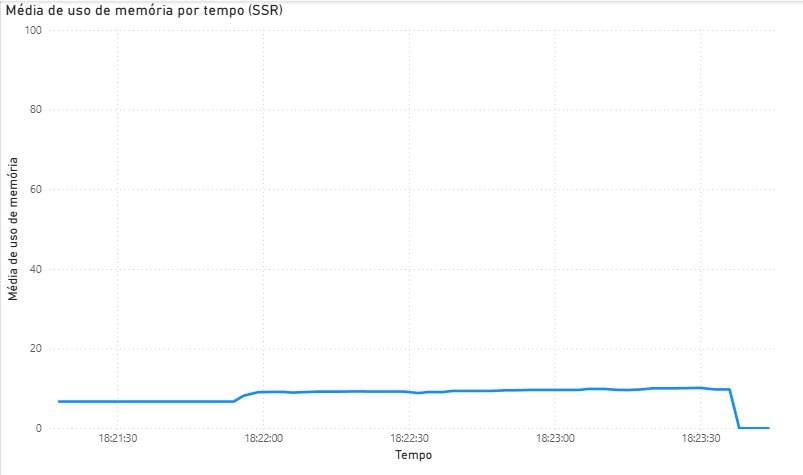
\includegraphics[width=0.9\textwidth]{media/uso_cpu_ssr.jpeg}
  \legend{Fonte: os autores.}
  \label{fig:ssr-cpu}
\end{figure}

\begin{figure}[H]
  \centering
  \caption{Média de uso de memória por tempo (\acrshort{ssr})}
  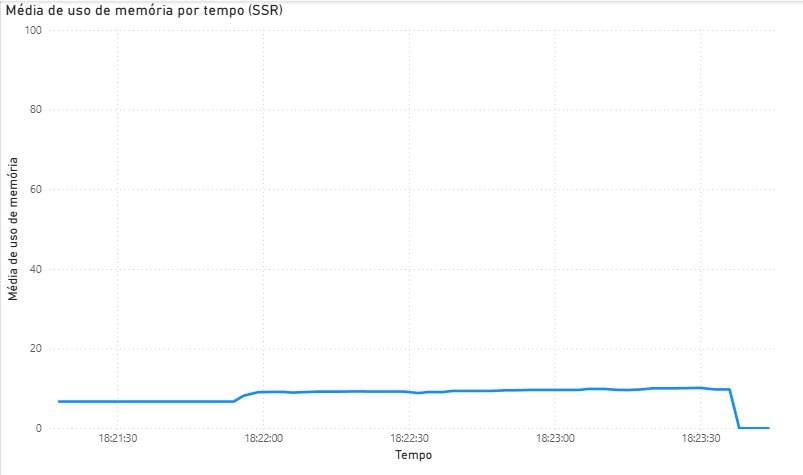
\includegraphics[width=0.9\textwidth]{media/uso_memoria_ssr.jpeg}
  \legend{Fonte: os autores.}
  \label{fig:ssr-mem}
\end{figure}

\subsubsection*{Web Vitals (cliente)}
Conforme a \autoref{fig:ssr-webvitals}, as leituras de campo foram, em sua maioria, classificadas como \textit{good}. Os poucos casos de \textit{needs-improvement} concentraram-se em \acrshort{lcp} e \acrshort{inp}, e houve uma fração reduzida de \acrshort{fcp} em \textit{poor} — efeito compatível com custos de \textit{hydration} e com elementos visuais de grande porte na dobra (imagens \emph{hero}). Em relação às metas adotadas, os resultados situam-se, em geral, próximos ou dentro dos limiares de referência: \acrshort{lcp} $\leq 2{,}5$\,s; \acrshort{cls} $\leq 0{,}10$; \acrshort{inp} $\leq 200$\,ms; \acrshort{ttfb} $\leq 800$\,ms.

\begin{figure}[H]
  \centering
  \caption{Classificação das métricas de desempenho (\acrshort{ssr}) com Web Vitals}
  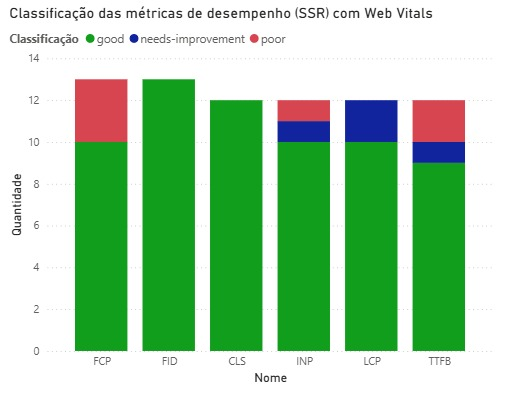
\includegraphics[width=0.9\textwidth]{media/metricas_ssr_web_vitals.jpeg}
  \legend{Fonte: os autores.}
  \label{fig:ssr-webvitals}
\end{figure}

\subsubsection*{Lighthouse (apoio diagnóstico)}
Para explicar variações residuais e priorizar melhorias, auditamos as rotas \emph{home}, \emph{busca} e \emph{detalhe} no modo \emph{Navigation} do Chrome DevTools, considerando três indicadores: \textbf{TBT}, \textbf{Acessibilidade} e \textbf{SEO}.
A Tabela~\ref{tab:lh-ssr} consolida as \textbf{medianas} observadas nos relatórios HTML anexados (\texttt{ssrMobile.html}, \texttt{ssrMobileBusca.html}, \texttt{ssrtestePage.html}).

\begin{table}[H]
\centering
\caption{Lighthouse (SSR) — mediana por rota}
\label{tab:lh-ssr}
\begin{tabular}{|l|c|c|c|}
\hline
\textbf{Rota} & \textbf{TBT (ms)} & \textbf{Acessibilidade (\%)} & \textbf{SEO (\%)} \\
\hline
Home    & 12 & 95  & 100 \\
Busca   & 10 & 99  & 100 \\
Detalhe & 0--7\footnotemark[1] & 100 & 100 \\
\hline
\end{tabular}
\end{table}
\footnotetext[1]{Variações muito baixas entre execuções; mediana $\approx$ 5\,ms.}

\noindent \textit{Leitura.}
(i) \textbf{TBT} muito abaixo da meta interna ($<200$\,ms) em todas as rotas, corroborando \acrshort{inp} em \textit{good};
(ii) \textbf{Acessibilidade} alta (95--100\%), com ajustes residuais (hierarquia de headings, foco visível, rótulos) de fácil endereçamento;
(iii) \textbf{SEO} consistente (100\%), indicando sinalização adequada (título, \emph{meta description}, \texttt{canonical}, \texttt{robots}, \texttt{viewport}) — aspecto particularmente relevante no fluxo SSR.

\subsubsection*{Síntese (SSR)}
Servidor com CPU/RAM contidos; \emph{Web Vitals} majoritariamente \textit{good}, com atenção pontual a \acrshort{lcp}/\acrshort{fcp} em páginas com imagens destacadas e pós-hidratação; \emph{Lighthouse} confirma \textbf{TBT} reduzido e \textbf{altos escores} de \textbf{Acessibilidade} e \textbf{SEO}, sustentando o SSR para páginas públicas sensíveis à descoberta.




\subsection{Resultados para CSR}
\label{subsec:resultados-csr}

\subsubsection*{Recursos do servidor}
O contêiner da \emph{SPA} apresentou \textbf{CPU} muito baixa e estável, com oscilações discretas e picos inferiores a 5\% (\autoref{fig:csr-cpu}). A \textbf{memória} permaneceu praticamente constante e em patamar reduzido durante todo o ensaio, coerente com a entrega estática e a execução da lógica no cliente (\autoref{fig:csr-mem}). Não se observaram sinais de saturação.

\begin{figure}[H]
\centering
\caption{Média de uso de CPU por tempo (\acrshort{csr})}
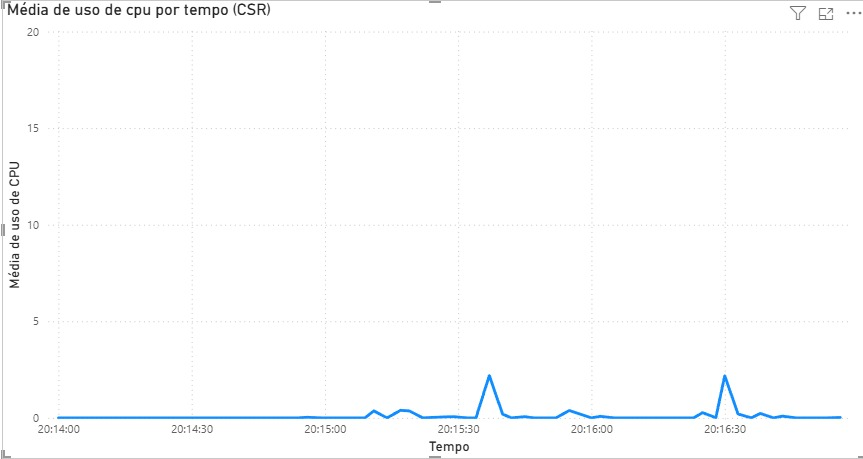
\includegraphics[width=0.9\textwidth]{media/uso_cpu_csr.jpeg}
\legend{Fonte: os autores.}
\label{fig:csr-cpu}
\end{figure}

\begin{figure}[H]
\centering
\caption{Média de uso de memória por tempo (\acrshort{csr})}
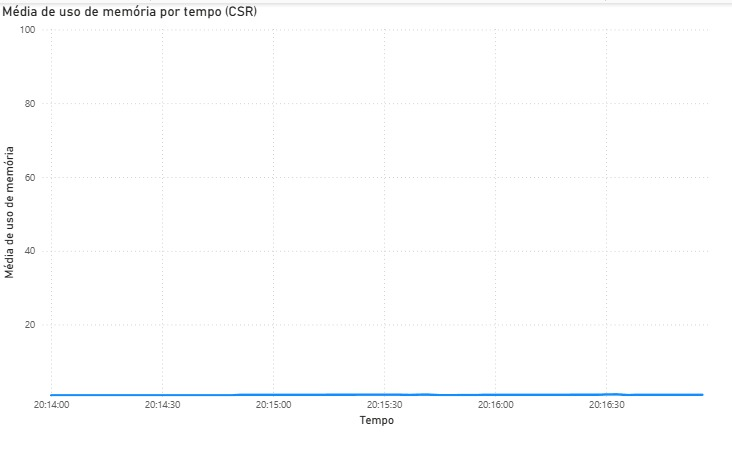
\includegraphics[width=0.9\textwidth]{media/uso_memoria_csr.jpeg}
\legend{Fonte: os autores.}
\label{fig:csr-mem}
\end{figure}

\subsubsection*{Web Vitals (cliente)}
As leituras de campo indicam \textbf{predomínio de \textit{good}} em \acrshort{ttfb}, \acrshort{fcp}, \acrshort{lcp} e \acrshort{inp} (\autoref{fig:csr-webvitals}). O ponto fora da curva é a \textbf{\acrshort{cls}}, com concentrações em \textit{poor}. O padrão é típico de SPAs quando ocorrem \emph{layout shifts} durante a hidratação ou quando imagens/slots não reservam espaço antes do carregamento (dimensões ausentes, fontes sem \emph{preload}, inserções acima da dobra). Em relação às metas, as leituras ficaram, em geral, dentro ou próximas dos limiares de referência (\acrshort{lcp} $\leq 2{,}5$\,s; \acrshort{cls} $\leq 0{,}10$; \acrshort{inp} $\leq 200$\,ms; \acrshort{ttfb} $\leq 800$\,ms), com a ressalva da \acrshort{cls}.

\begin{figure}[H]
\centering
\caption{Classificação das métricas de desempenho (\acrshort{csr}) com Web Vitals}
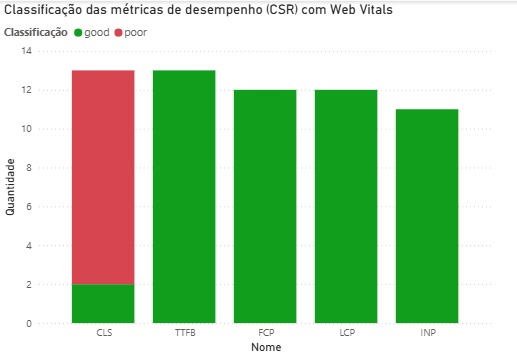
\includegraphics[width=0.9\textwidth]{media/metricas_csr_web_vitals.jpeg}
\legend{Fonte: os autores.}
\label{fig:csr-webvitals}
\end{figure}

\subsubsection*{Lighthouse (apoio diagnóstico)}
Para explicar oscilações residuais e orientar priorizações, auditamos as rotas críticas no \emph{Chrome DevTools} (modo \emph{Navigation}), com três indicadores: \textbf{TBT}, \textbf{Acessibilidade} e \textbf{SEO}.

\noindent \textit{Achados.}
\begin{itemize}
  \item \textbf{TBT}: manteve-se em patamar \textbf{muito baixo} (dezenas de milissegundos) nas páginas inspecionadas, consistente com \acrshort{inp} \textit{good}.
  \item \textbf{Acessibilidade}: escores altos na \emph{home} (93--94\,\%), com ajustes residuais (hierarquia de \emph{headings}, foco visível, rótulos/\textit{alt}) — valores observados nos relatórios “Home (Web)” e “Home (Mobile)”.
  \item \textbf{SEO}: a \emph{home} registrou \textasciitilde{}83\,\% (Web e Mobile), sugerindo oportunidades pontuais (por exemplo, \emph{meta description}/\texttt{canonical}/\texttt{robots}/\texttt{hreflang}, quando aplicável).
\end{itemize}

\noindent \textit{Leitura.} Em conjunto, os relatórios apontam que o gargalo do \textbf{CSR} não está em bloqueio de \emph{main thread} (TBT baixo), mas em \textbf{estabilidade visual} e em alguns sinais de \textbf{SEO}. Na prática, os seguintes ajustes tendem a capturar os ganhos: (i) reservar dimensões de imagens e \emph{cards} acima da dobra (\texttt{width}/\texttt{height} ou \texttt{aspect-ratio}); (ii) \emph{preload} de fontes e imagens \emph{hero} (com \texttt{font-display: swap}); (iii) evitar inserções DOM acima da dobra durante a hidratação; (iv) completar metadados de SEO (título/descrição/\texttt{canonical}/\texttt{robots}) e revisar indexabilidade.

\subsubsection*{Síntese (CSR)}
Servidor praticamente ocioso (CPU e RAM baixos); \emph{Web Vitals} em boa forma para \acrshort{ttfb}/\acrshort{fcp}/\acrshort{lcp}/\acrshort{inp}, com atenção especial à \textbf{\acrshort{cls}}. O \emph{Lighthouse} confirmou \textbf{TBT reduzido}, \textbf{Acessibilidade} alta e \textbf{SEO} com melhorias de rápida implementação, coerentes com o perfil de \textbf{SPA} e suas responsabilidades no cliente.

\subsection{Comparação entre SSR e CSR}
\label{subsec:comparacao-ssr-csr}

Esta seção compara, de forma integrada, experiência do usuário (\emph{Web Vitals} em campo), diagnóstico laboratorial (Lighthouse: TBT, Acessibilidade e SEO) e custo operacional (CPU/Memória nos contêineres). A leitura está ancorada nas medianas (p50) e, quando pertinente, no p95 dos cenários \textbf{home}, \textbf{busca} e \textbf{detalhe}.

\begin{table}[H]
\centering
\caption{Síntese comparativa dos resultados (SSR $\times$ CSR) neste estudo}
\label{tab:comparativo-ssr-csr}
\begin{tabular}{|p{4.2cm}|p{5.2cm}|p{5.2cm}|}
\hline
\textbf{Aspecto} & \textbf{SSR (MPA/Next.js)} & \textbf{CSR (SPA/React)} \\
\hline
\textbf{CPU no servidor} & Baixa e estável (\textit{$\sim$8--13\%}), sem picos relevantes. & Muito baixa; oscilações discretas com picos $<5\%$. \\
\hline
\textbf{Memória no servidor} & Estável, variação estreita; queda apenas ao término dos testes. & Muito baixa e praticamente constante. \\
\hline
\textbf{Web Vitals (campo)} & Predominância de \textit{good}; pequenos trechos \textit{needs-improvement} em \textbf{LCP}/\textbf{INP} e fração \textit{poor} em \textbf{FCP} (páginas com imagens \emph{hero} e pós-hidratação). & \textbf{TTFB}/\textbf{FCP}/\textbf{LCP}/\textbf{INP} majoritariamente \textit{good}; \textbf{CLS} com ocorrências \textit{poor} (shifts na montagem/hidratação e elementos sem reserva de espaço). \\
\hline
\textbf{Lighthouse: TBT} & \textbf{Muito baixo} (home $\approx$12\,ms; busca $\approx$10\,ms; detalhe $\approx$5\,ms). & \textbf{Muito baixo} (ordem de dezenas de ms na home). \\
\hline
\textbf{Lighthouse: Acessibilidade} & \textbf{Alta} (95--100\%). & \textbf{Alta} (93--94\% na home). \\
\hline
\textbf{Lighthouse: SEO} & \textbf{100\%} nas rotas auditadas. & \textbf{$\sim$83\%} na home; indica metadados/sinalizações a completar. \\
\hline
\textbf{Leitura operacional} & Parte da renderização no servidor melhora \textbf{TTFB}/\emph{first paint} e favorece \textbf{SEO}; cuidado com \emph{hydration} e imagens de grande porte. & Renderização no cliente alivia o servidor e mantém \textbf{TBT/INP} baixos; requer disciplina de layout para evitar \textbf{CLS} e ajustes de \textbf{SEO}. \\
\hline
\end{tabular}
\end{table}

\subsubsection{Pontos fortes do SSR.}
(i) \textbf{Tempo até primeira resposta/primeiro conteúdo.} O HTML pré-renderizado reduz o tempo de exibição inicial, o que se refletiu em \textit{TTFB}/\textit{FCP} consistentes e \textbf{TBT} residual nas auditorias.  
(ii) \textbf{Descoberta e rastreabilidade.} \textbf{SEO} com 100\% nas rotas testadas, reforçando a adequação do SSR para páginas públicas e conteúdo editorial.  
(iii) \textbf{Acessibilidade.} Escores elevados (95--100\%) indicam que a estrutura entregue pelo servidor chega semanticamente “pronta” ao cliente.  
(iv) \textbf{Previsibilidade de performance.} Em cenários com rede/CPU do cliente mais limitados, a renderização no servidor reduz o risco de longas tarefas no \emph{main thread} do navegador.

\subsubsection{Pontos fracos do SSR.}
(i) \textbf{Custo de hidratação.} Após o HTML inicial, a ativação dos componentes pode degradar \textbf{LCP}/\textbf{FCP} em páginas com imagens \emph{hero} e muito JS.  
(ii) \textbf{Custo no servidor (ainda que baixo).} O processamento por requisição eleva discretamente \textbf{CPU}/\textbf{memória} no host frente ao CSR.  
(iii) \textbf{Complexidade de build/deploy.} Estratégias como \emph{streaming}, \emph{partial/targeted hydration} e \emph{Server Components} elevam a complexidade de arquitetura.

\subsubsection{Pontos fortes do CSR.}
(i) \textbf{Interatividade contínua.} Navegação sem recarregar página, com \textbf{TBT/INP} baixos nas auditorias e nos dados de campo.  
(ii) \textbf{Custo operacional.} \textbf{CPU/memória} do servidor permanecem muito baixos: entrega estática + execução no cliente.  
(iii) \textbf{Escalabilidade horizontal simples.} Conteúdo estático facilita cache/CDN, reduzindo pressão no backend.

\subsubsection{Pontos fracos do CSR.}
(i) \textbf{Estabilidade visual.} \textbf{CLS} apresentou ocorrências \textit{poor}; o risco de \emph{layout shifts} aumenta quando não há reserva de espaço para mídia e quando há inserções acima da dobra na hidratação.  
(ii) \textbf{Sinais de SEO.} Escores \textasciitilde83\% na home (Lighthouse) indicam metadados/sinalizações a completar (p.\,ex., \emph{meta description}, \texttt{rel=canonical}, \texttt{robots}, \texttt{hreflang} quando aplicável).  
(iii) \textbf{Dependência de JS no cliente.} Em dispositivos muito modestos, o custo de montar a aplicação pode afetar \textit{FCP}/\textit{LCP} se o \emph{bundle} não for estritamente otimizado.

\subsubsection{Observação sobre a Ausência do FID em CSR.} 
No \acrshort{csr}, o \acrfull{fid} não é capturado da maneira tradicional, pois a página precisa ser 'hidratada' pelo JavaScript antes de se tornar completamente interativa. Esse processo de hidratação impede que o \acrshort{fid} meça corretamente a primeira interação do usuário, tornando-o menos relevante em ambientes \acrshort{csr}. Por isso, o \acrfull{inp} é utilizado como métrica alternativa, já que ele captura o tempo de resposta entre a interação do usuário e a atualização visual da página, oferecendo uma avaliação mais precisa da interatividade contínua, o que é especialmente importante em páginas altamente dinâmicas como as renderizadas no cliente.

\subsection{Discussão}
\label{subsec:discussao-comparativa}
\textbf{(i) Recursos do servidor.} O \acrshort{ssr} consumiu levemente mais \textbf{CPU/memória} (ainda baixos) do que o \acrshort{csr}, resultado esperado do processamento por requisição. O \acrshort{csr}, por sua vez, opera praticamente como \emph{static hosting}, com custo mínimo no host. \\
\textbf{(ii) Experiência do usuário.} Em \acrshort{ssr}, a entrega inicial é perceptivelmente rápida e os escores de \textbf{SEO} e \textbf{Acessibilidade} são superiores; as pequenas perdas em \textbf{LCP}/\textbf{FCP} aparecem em páginas com imagens grandes e após a hidratação. Em \acrshort{csr}, \textbf{TTFB}/\textbf{FCP}/\textbf{LCP}/\textbf{INP} resultaram majoritariamente \textit{good}, e o \textbf{TBT} foi baixo; o principal cuidado é a \textbf{CLS}. \\
\textbf{(iii) Coerência entre campo e laboratório.} Os \textit{Web Vitals} em campo (usuário real) e o \textbf{TBT} do Lighthouse (laboratório) convergiram: baixo bloqueio de \emph{main thread} nos dois modelos. As divergências localizam-se em \textbf{CLS} (CSR) e \textbf{SEO} (CSR $<$ SSR), que são áreas classicamente sensíveis à estratégia de renderização.

\subsection{Implicações práticas}
\begin{itemize}
  \item \textbf{Priorizar SSR} quando: páginas públicas dependentes de \textbf{SEO}, conteúdo editorial/comercial, catálogos indexáveis e cenários em que \textbf{TTFB} e \textbf{exibição inicial} são críticos para engajamento e descoberta.
  \item \textbf{Priorizar CSR} quando: aplicações altamente interativas (dashboards, sistemas internos), requisitos fortes de navegação fluida no cliente e \textbf{custo de servidor} deve permanecer mínimo.
\end{itemize}

\subsection{Ajustes recomendados}
\textbf{SSR (mitigar LCP/INP).} Otimizar e dimensionar imagens (usar \texttt{priority} para \emph{hero} e \emph{lazy} abaixo da dobra), considerar \emph{streaming}/\emph{partial hydration}/\emph{Server Components}, reduzir JS não crítico e declarar \texttt{preload}/\texttt{dns-prefetch} para recursos essenciais. \\
\textbf{CSR (mitigar CLS e elevar SEO).} Reservar dimensões de mídia (\texttt{width}/\texttt{height} ou \texttt{aspect-ratio}); evitar inserções acima da dobra durante a hidratação; \texttt{font-display: swap} com \emph{preload} de fontes e imagens \emph{hero}; placeholders do tamanho final; completar metadados e sinalizações (\emph{title}/\emph{description}/\texttt{canonical}/\texttt{robots}/\texttt{hreflang} quando aplicável).

\subsection{Síntese}
No cenário testado, \textbf{SSR} e \textbf{CSR} entregaram boa experiência de uso com \textbf{baixa pressão de recursos}. O \textbf{SSR} destacou-se por \textbf{SEO} e \textbf{exibição inicial} mais previsível; o \textbf{CSR} reduziu o \textbf{custo no servidor} e manteve \textbf{TBT/INP} baixos, com a contrapartida de maior propensão a \textbf{CLS} e sinais de \textbf{SEO} a complementar. A decisão deve considerar \textbf{perfil de tráfego}, \textbf{exigência de descoberta} e \textbf{tipo de interação}, aplicando as otimizações para mitigar os pontos fracos identificados em cada abordagem.


\chapter{Conclusão}
\label{cap:conclusao}

Este trabalho de conclusão de curso realizou uma análise comparativa aprofundada entre as arquiteturas de renderização no lado do cliente (\acrfull{csr}) e no lado do servidor (\acrfull{ssr}), com o intuito de dissecar suas implicações na performance, na experiência do usuário e nos desafios de implementação. A partir do desenvolvimento e teste de duas versões da plataforma "WallTech" em um ambiente controlado, foi possível validar empiricamente os trade-offs inerentes a cada abordagem.

A investigação confirmou que a escolha arquitetônica molda fundamentalmente a jornada do usuário. A abordagem \acrshort{ssr} demonstrou ser superior na fase inicial da interação, entregando um primeiro conteúdo visual (\acrfull{fcp}) de forma notavelmente rápida e garantindo excelente estabilidade visual (\acrfull{cls}). Essa performance inicial, aliada à otimização natural para mecanismos de busca (\acrfull{seo}), a torna ideal para aplicações onde a primeira impressão e a descoberta de conteúdo são críticas.

Em contrapartida, o \acrshort{csr} redefiniu a experiência após o carregamento inicial, oferecendo uma interatividade superior e navegação quase instantânea, refletida em um baixo \acrfull{inp}, que emula a fluidez de um aplicativo nativo. Contudo, essa vantagem vem ao custo de um carregamento inicial mais lento e de uma maior suscetibilidade a instabilidades de layout, exigindo uma disciplina de desenvolvimento rigorosa para mitigar os pontos fracos da abordagem.

Portanto, este trabalho cumpriu seus objetivos ao demonstrar, com dados concretos, que a decisão entre \acrshort{csr} e \acrshort{ssr} é uma escolha estratégica. Ela se resume a um trade-off fundamental sobre onde a carga computacional deve residir e o que se deve priorizar: a velocidade da primeira renderização e a indexabilidade do \acrshort{ssr}, ou a interatividade contínua e a redução de custos de servidor do \acrshort{csr}.

A principal contribuição desta pesquisa reside na sua metodologia sistemática e reprodutível, que oferece um roteiro prático para a avaliação comparativa de arquiteturas frontend. Como limitação, reconhece-se que o ambiente de teste local, embora essencial para o controle experimental, não captura a variabilidade de redes e dispositivos do mundo real.

Para trabalhos futuros, sugere-se a análise de arquiteturas híbridas, como \acrfull{ssg} e \acrfull{isr}, que prometem unir o melhor dos dois mundos. Adicionalmente, seria de grande valia investigar o impacto de paradigmas emergentes, como os \textit{React Server Components} e o \textit{Streaming SSR}, e complementar os dados quantitativos com estudos qualitativos de usabilidade, para aprofundar a compreensão sobre a percepção real do usuário.

\postextual

\bibliography{Referencias}

% Imprime uma página indicando o início dos apêndices
% \partapendices
%\part*{Apêndices}

%\begin{apendicesenv}

%
\chapter{Questionário de Avaliação do Protótipo}









%\end{apendicesenv}

%\begin{anexosenv}

%


%\end{anexosenv}

\end{document}
